%=====================================================================
% Modelo de datos
%   Un archivo por subsección en modelo/, para que un cambio en el
%   modelo toque solo el archivo de la parte que cambia.
%
%   Lo que viene de bd/tex se genera a partir de bd/crear_tablas.sql con
%   bd/generar_tablas.ps1, y los diagramas de er/salida a partir de
%   er/modelos con er/generar.py. Si cambia el esquema, se edita el
%   script SQL o el modelo del diagrama y se vuelven a generar; esos
%   archivos no se editan a mano.
%=====================================================================
%=====================================================================
% Modelo de datos · Introducción y convenciones
%=====================================================================
\section*{Modelo de datos}
\addcontentsline{toc}{section}{Modelo de datos}

Esta sección define el esquema de la base de datos de \sistema{} en SQL Server (\mbox{CON-04}). Parte del diagrama entidad-relación inicial y lo lleva hasta las estructuras que exigen los casos de uso, el análisis CRUD y las decisiones de diseño: presenta el diagrama entidad-relación actualizado, identifica las entidades, sus atributos, sus llaves primarias y foráneas, las relaciones entre ellas con su cardinalidad, y justifica que el resultado está en tercera forma normal. Termina con el usuario con el que el Servidor de partidas se conecta a la base.

El esquema tiene \bdNumTablas{} entidades, \bdNumColumnas{} atributos y \bdNumForaneas{} llaves foráneas. Todas las tablas cumplen la tercera forma normal y \bdNumFNBC{} cumplen además la forma normal de Boyce-Codd; las dos que no, se explican en la sección de normalización.

La sección de implementación, que sigue a esta, crea la base con tres scripts: \at{bd/crear\_base\_datos.sql} crea la base y el usuario de conexión; \at{bd/crear\_tablas.sql}, las tablas, sus restricciones, los índices y los procedimientos almacenados de las eliminaciones físicas; e \at{bd/insertar\_datos\_prueba.sql} carga los catálogos y un conjunto de datos de prueba. Las tablas de atributos, de llaves y de relaciones de esta sección no se escribieron a mano: se generan a partir de \at{bd/crear\_tablas.sql} con \at{bd/generar\_tablas.ps1}, de modo que el documento y la base no pueden contradecirse. El mismo generador exporta el esquema a \at{er/esquema.json}, del que parten los diagramas entidad-relación. Si el esquema cambia, se edita el script y se vuelven a generar las tablas y los diagramas.

Se siguen las convenciones del análisis CRUD: las entidades se escriben en cursiva y los atributos en tipografía de código, sin acentos ni eñes porque son identificadores de la base de datos. Además:

\begin{reglas}
  \item \textbf{Nombres.} Tablas en singular, con la misma forma que en los casos de uso (\textit{Usuario}, \textit{EstadisticaModo}); atributos en minúsculas separados por guion bajo.
  \item \textbf{Fechas.} Todas en UTC, con \at{DATETIME2}. El servidor las convierte a la hora local solo para mostrarlas.
  \item \textbf{Texto.} Todo lo que escribe o lee una persona es \at{NVARCHAR}, en Unicode (\mbox{CON-05}). Los códigos de estado y de dominio son \at{VARCHAR}, porque solo los lee la aplicación. La base usa una intercalación UTF-8, así que los dos tipos admiten la ñ, los acentos y cualquier carácter Unicode (\mbox{D-21}). Nada se guarda traducido: cada fila de catálogo guarda un \at{codigo}, la clave de su nombre en los diccionarios de recursos.
  \item \textbf{Secretos.} Contraseñas, tokens y códigos se guardan como resumen criptográfico en \at{VARBINARY}; ninguna columna los contiene en claro (\mbox{CU-01} \mbox{RN-02}).
  \item \textbf{Dominios.} Los valores permitidos de cada estado, tipo o ámbito que se listan en las descripciones están declarados en la base con restricciones \at{CHECK}.
\end{reglas}

%=====================================================================
% Modelo de datos · Del diagrama entidad-relación al modelo
%=====================================================================
\subsection*{Del diagrama entidad-relación al modelo}
\addcontentsline{toc}{subsection}{Del diagrama entidad-relación al modelo}

El diagrama entidad-relación de partida, que se reproduce al final de esta subsección, tiene seis entidades —\textit{Usuario}, \textit{Skin}, \textit{Estadísticas}, \textit{Partida}, \textit{Reporte} y \textit{Baneo}— y nueve relaciones. Es anterior a los casos de uso, y varias decisiones de diseño lo cambiaron después (\mbox{D-02} a \mbox{D-06}). La tabla indica qué fue de cada elemento del diagrama; el diagrama actualizado está en la subsección siguiente. Todo lo que el diagrama no tenía —sesiones, tokens, bitácoras, relaciones entre jugadores, salas, economía y tutorial— lo exigen los casos de uso, y la Matriz 1 de trazabilidad indica cuál.

\begin{center}\small
\begin{longtable}{|L{0.21\textwidth}|L{0.30\textwidth}|L{0.39\textwidth}|}
\hline
\textbf{Elemento del diagrama} & \textbf{En el modelo} & \textbf{Qué cambió y por qué} \\ \hline
\endfirsthead
\hline
\textbf{Elemento del diagrama} & \textbf{En el modelo} & \textbf{Qué cambió y por qué} \\ \hline
\endhead
\textit{Usuario} & \textit{Usuario} & Se elimina el atributo compuesto \at{nombre\_completo} y, con él, \at{nombre}, \at{apellido\_paterno} y \at{apellido\_materno}, junto con \at{region}: ningún flujo los usa (\mbox{D-06}). Se elimina \at{edad}, que es derivada. \at{contraseña} pasa a \at{contrasena\_hash} y \at{contrasena\_sal}. Se añaden \at{tipo\_cuenta} para el invitado (\mbox{D-02}), \at{rol}, y los datos del bloqueo, la verificación y la progresión. \\ \hline
\textit{Skin} & \textit{Ranura}, \textit{ObjetoCosmetico} & Un solo tipo de skin no alcanza para seis ranuras de personalización (\mbox{D-03}). El atributo \at{tipo} del skin se convierte en la entidad \textit{Ranura}; \at{costo} pasa a \at{precio}. \\ \hline
Posee (N:M) & \textit{UsuarioObjeto} & Se conserva como entidad asociativa con su \at{fecha\_obtencion} y gana \at{origen}. \\ \hline
Equipa (N:1) & \textit{Equipamiento} & Un skin equipado por usuario pasa a ser un objeto equipado por cada ranura: una fila por usuario y ranura. \\ \hline
\textit{Estadísticas}, Tiene (1:1) & \textit{Modo}, \textit{EstadisticaModo} & El elo y los contadores son por modo (\mbox{D-04}), así que la relación deja de ser 1:1: hay una fila por usuario y modo. Se elimina \at{porcentaje\_victorias}, que es derivado. \\ \hline
\textit{Partida} & \textit{Partida} & \at{num\_jugadores} pasa a \textit{Modo}, del que depende. \at{duracion} se elimina porque se calcula. Se añaden \at{tipo}, \at{forma\_termino}, el reloj y los datos de las partidas contra la IA (\mbox{D-12}). \\ \hline
Participa (N:M, 2 a 4) & \textit{Participacion} & \at{color\_ficha} pasa a \at{simbolo\_peon} y \at{barreras\_restantes} a \at{muros\_restantes}. Se añaden el elo de entrada y de salida, el reloj y el estado de conexión. La cardinalidad baja a 1 a 4, porque en una partida contra la IA solo participa el jugador. \\ \hline
\textit{Reporte}, Emite (1:N), Señala (N:1), Sobre (N:1) & \textit{Reporte}, \textit{MotivoReporte} & Las tres relaciones quedan como las llaves foráneas \at{id\_denunciante}, \at{id\_reportado} e \at{id\_partida}; la partida adjunta tiene que ser una que jugaron los dos (\mbox{CU-42} \mbox{RN-09}). El \at{motivo} en texto pasa a un catálogo; \at{estado\_reporte} pasa a \at{estado} con el moderador que lo revisa. \\ \hline
\textit{Baneo}, Recibe (1:N), Origina (N:1) & \textit{Sancion}, \textit{Apelacion} & La sanción gana ámbito de cuenta o de chat (\mbox{D-05}). \at{num\_reportes} y \at{activo} se eliminan: el primero es un conteo y el segundo se deducía de las fechas. La relación Origina queda como \at{id\_reporte}. \\ \hline
\end{longtable}
\end{center}

\begin{landscape}
\subsubsection*{Diagrama original}
\addcontentsline{toc}{subsubsection}{Diagrama original}
El diagrama entidad-relación de partida, en notación de Chen, dibujado de nuevo a partir de su modelo (\at{er/\allowbreak{}modelos/\allowbreak{}original.py}) con los mismos renderizadores que los diagramas actualizados.
\begin{center}
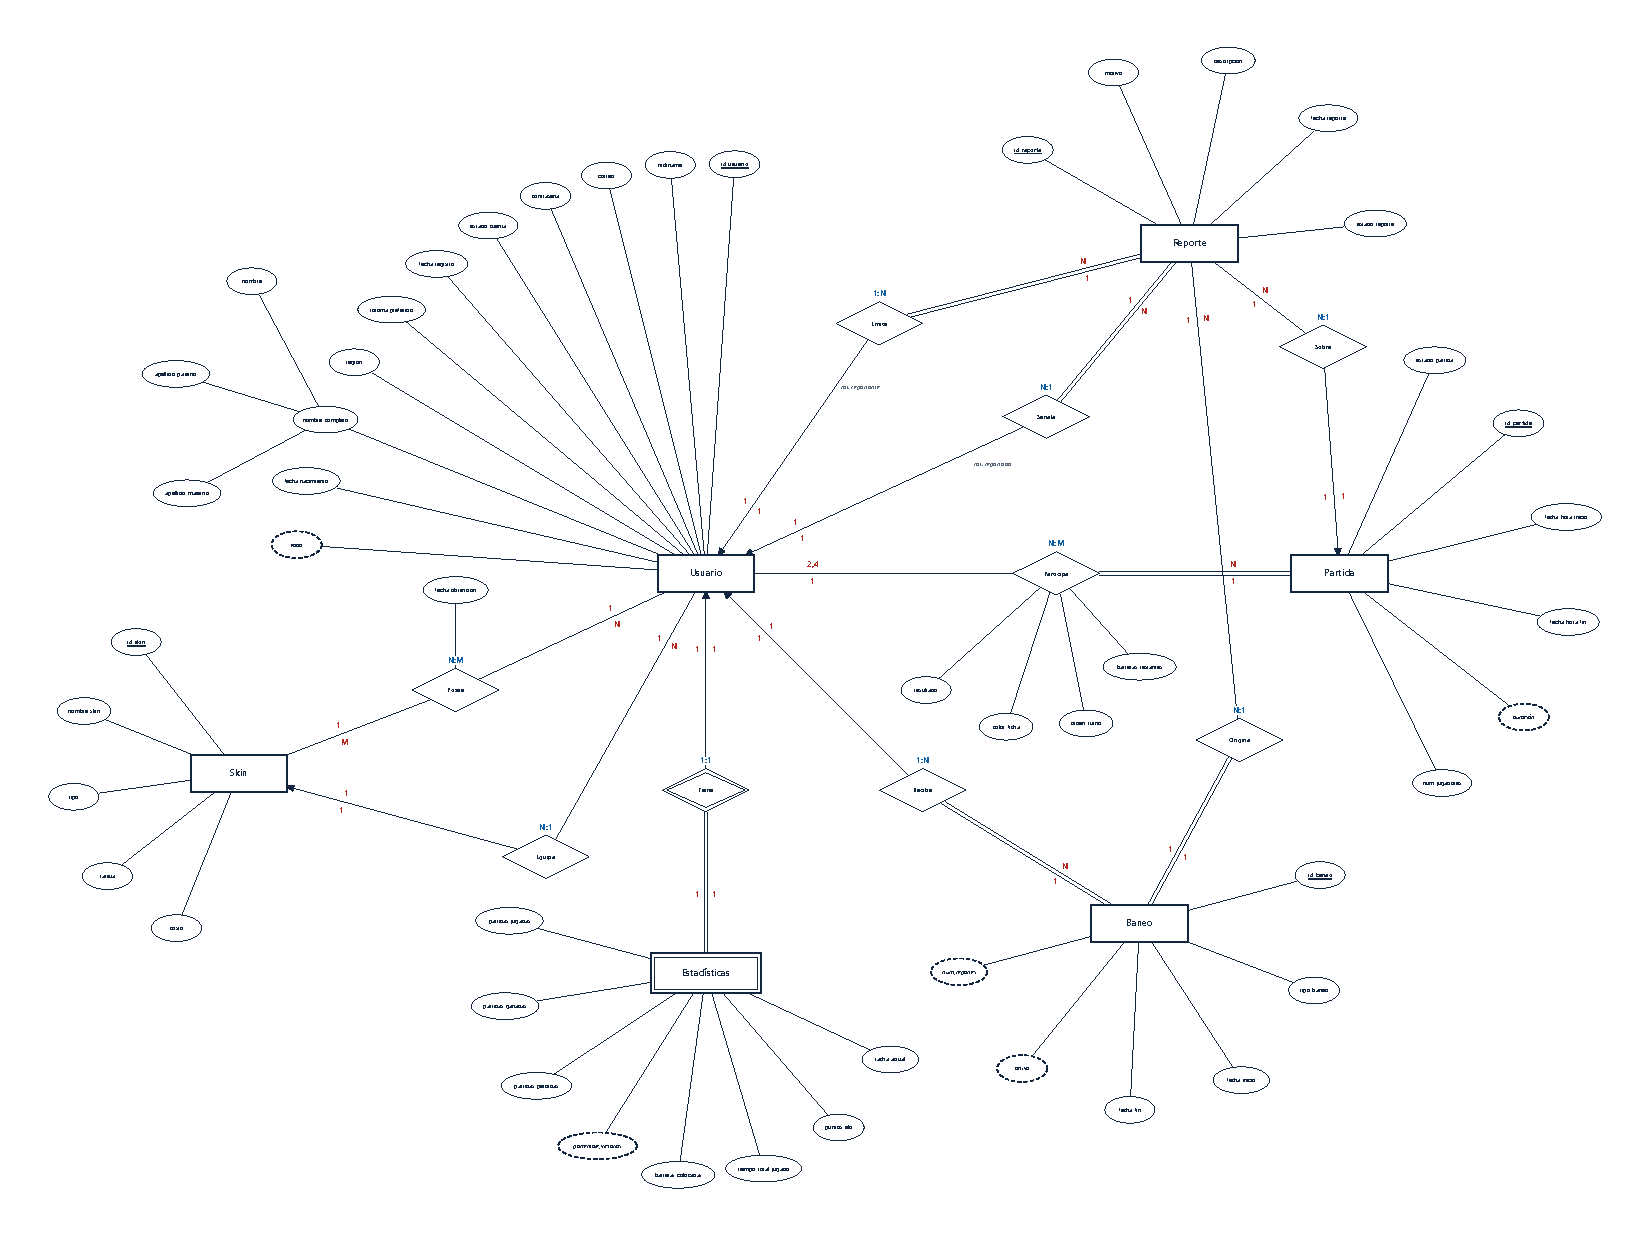
\includegraphics[width=\linewidth,height=0.8\textheight,keepaspectratio]{er/salida/original}
\end{center}
\end{landscape}

%=====================================================================
% Modelo de datos · Diagrama entidad-relación
%   Las figuras de er/salida se generan con er/generar.py a partir de
%   er/esquema.json (que exporta bd/generar_tablas.ps1) y de
%   er/diagramas.py. No se editan a mano.
%=====================================================================
\subsection*{Diagrama entidad-relación}
\addcontentsline{toc}{subsection}{Diagrama entidad-relación}

Los diagramas de esta subsección son el modelo actualizado, en la misma notación de Chen del diagrama original. No se dibujaron a mano: \at{er/generar.py} los construye a partir del esquema que exporta \at{bd/generar\_tablas.ps1}, de modo que muestran exactamente las tablas, columnas y llaves foráneas del script \at{bd/crear\_tablas.sql}. Cada uno existe además como archivo \at{.drawio}, editable en app.diagrams.net, en \at{er/salida}. Las figuras son vectoriales: los nombres de los atributos se leen ampliando el PDF, o en los \at{.svg} de la misma carpeta.

Un solo dibujo con \bdNumTablas{} entidades y \bdNumColumnas{} atributos no se podría leer, así que el modelo se presenta en una vista general, con todas las entidades y relaciones pero sin atributos, y en un diagrama por área con todos sus atributos. En cada diagrama de área aparecen también, sin atributos, las entidades de otras áreas que sus relaciones tocan; sus atributos están en el diagrama de su propia área.

\subsubsection*{Cómo se leen}
\addcontentsline{toc}{subsubsection}{Cómo se leen}

\begin{reglas}
  \item \textbf{Entidades.} Cada tabla es una entidad, dibujada como rectángulo. Las que se identifican por la llave de otra ---débiles, asociativas y dependientes, según la tabla de identificación de entidades--- llevan doble marco.
  \item \textbf{Relaciones.} Cada llave foránea es una relación, dibujada como rombo con un verbo. El rombo es doble cuando la relación es identificadora, es decir, cuando las columnas de la llave foránea forman parte de la llave primaria de la hija.
  \item \textbf{Atributos.} Son óvalos unidos a su entidad. Los de la llave primaria van subrayados; en una entidad débil, el subrayado marca su discriminador, como \at{numero\_jugada} en \textit{Jugada}. Los de línea punteada son las columnas calculadas. Las columnas de una llave foránea no se dibujan como atributos, porque las representa la relación.
  \item \textbf{Razón.} Sobre cada rombo va la razón (\at{1:N}, \at{N:1} o \at{1:1}), y la flecha apunta al lado 1. Se lee siguiendo la frase del rombo: «\textit{Usuario} abre \textit{Sesion}» es 1:N y «\textit{Reporte} señala a \textit{Usuario}» es N:1.
  \item \textbf{Pares de cardinalidad.} Junto a cada entidad van dos cifras. La de arriba se lee siguiendo la frase del rombo, del sujeto al objeto; la de abajo, al revés. El sujeto lleva arriba siempre 1.
  \item \textbf{Participación.} La doble línea marca participación total: toda fila de esa entidad participa en la relación. Del lado de la hija corresponde a una llave foránea obligatoria; del lado del padre, a una regla de negocio, como las estadísticas de cada modo y los objetos iniciales que el alta crea para todo usuario (\mbox{CU-02} \mbox{RN-06}). La línea simple marca participación parcial. En el archivo \at{.drawio} la doble línea oculta la flecha, porque draw.io no dibuja las dos cosas a la vez.
  \item \textbf{Papeles.} Cuando una entidad participa dos veces en relaciones con la misma otra entidad, cada línea lleva su papel en cursiva: el emisor y el destinatario de una invitación, el reportante y el reportado de un reporte.
  \item \textbf{Relación recursiva.} La única relación de una entidad consigo misma, la sanción que sustituye a otra (\mbox{CU-44} \mbox{RN-09}), se dibuja con dos líneas paralelas hacia \textit{Sancion}, una por papel.
\end{reglas}

Hay restricciones que ninguna notación de cardinalidad expresa y que el esquema garantiza de otro modo. Que una partida tenga uno, dos o cuatro participantes según su tipo y su modo lo garantiza la transacción que la crea (\mbox{CU-17} \mbox{RN-10}); que un usuario tenga una sola participación sin terminar (\mbox{D-11}), el índice único filtrado de \textit{Participacion}.

%---------------------------------------------------------------------
% Vista general
%---------------------------------------------------------------------
\clearpage
\subsubsection*{Vista general}
\addcontentsline{toc}{subsubsection}{Vista general}
Las \bdNumTablas{} entidades y sus \bdNumForaneas{} relaciones, sin atributos. \textit{Usuario} queda en el centro porque es la entidad de la que depende casi todo el modelo.
\begin{center}
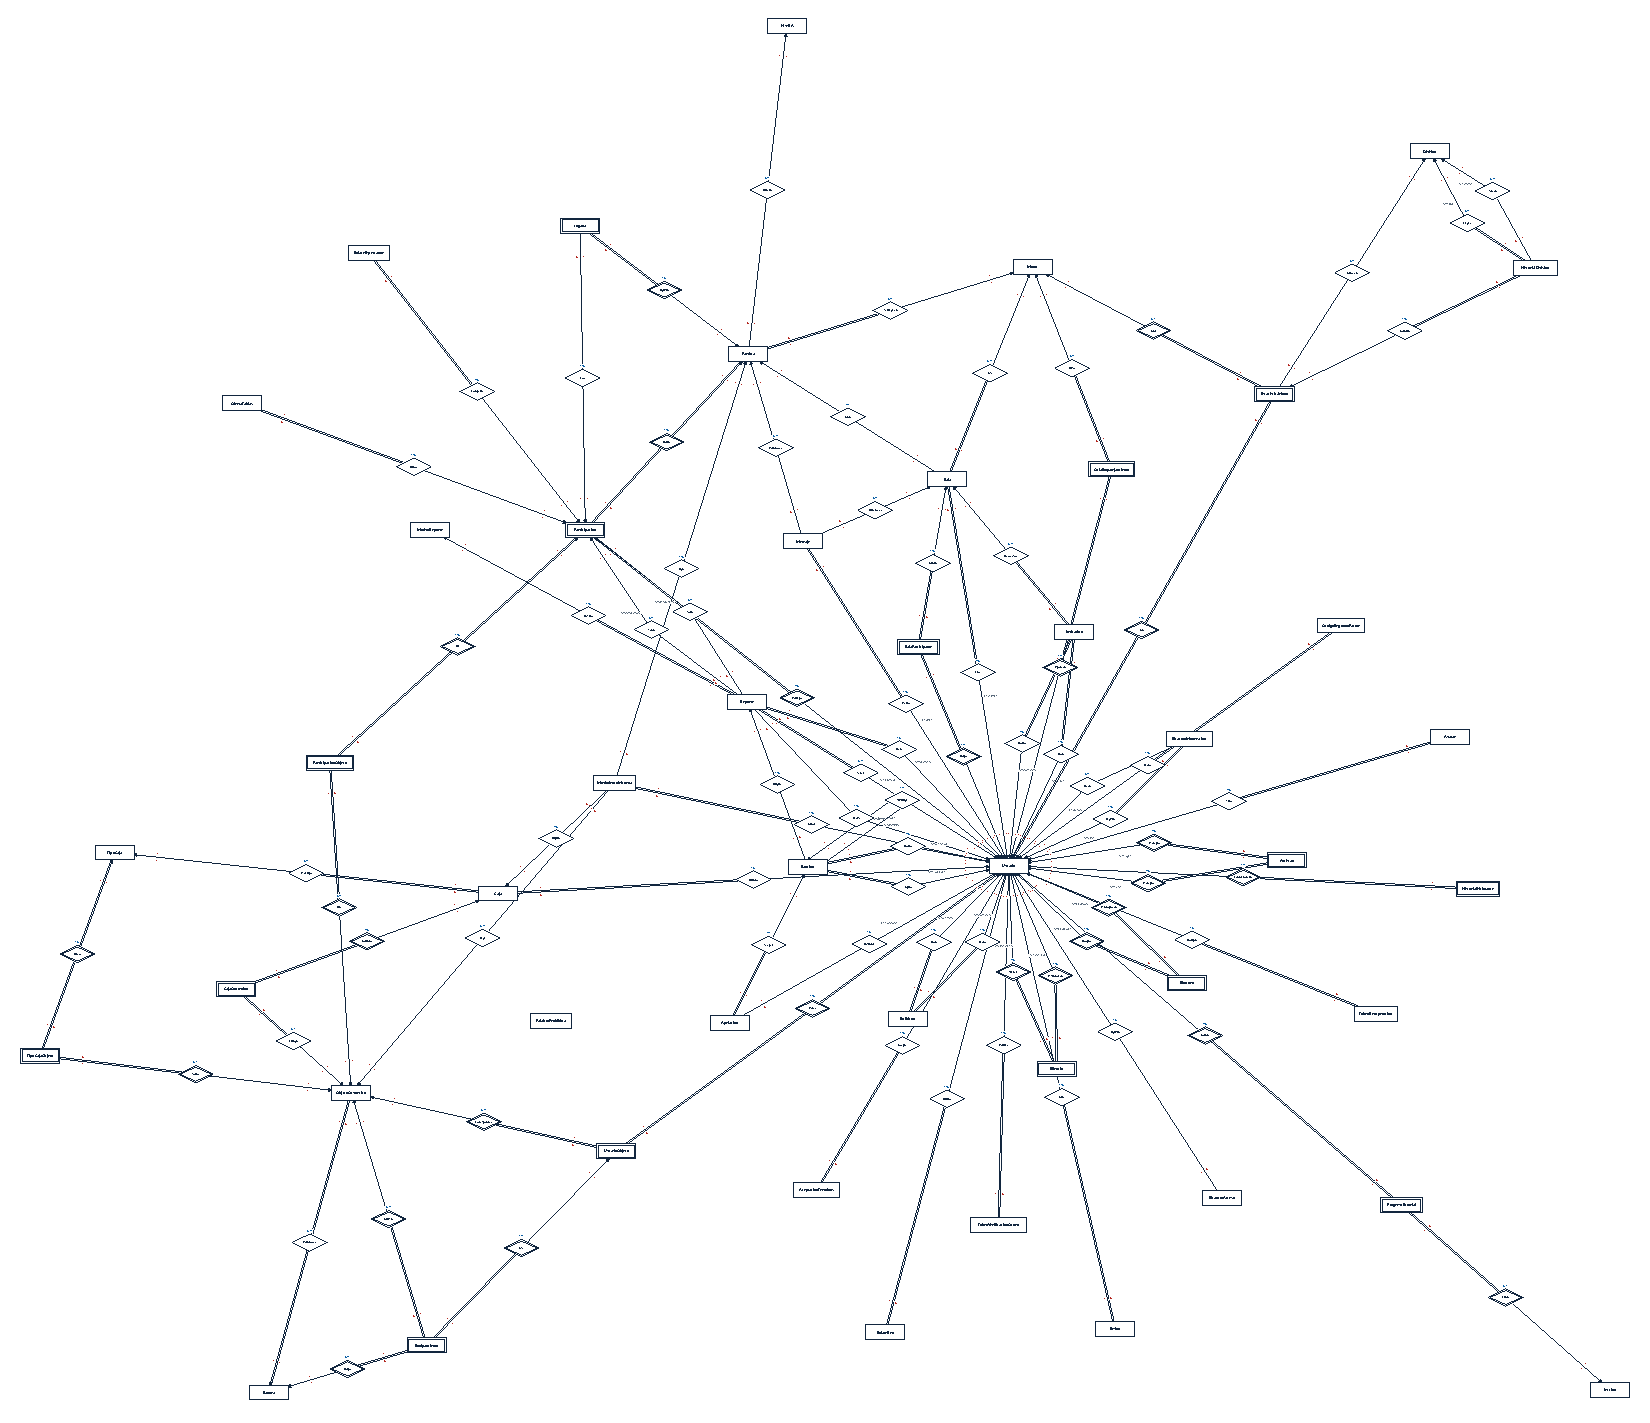
\includegraphics[width=\linewidth,height=0.82\textheight,keepaspectratio]{er/salida/general}
\end{center}

%---------------------------------------------------------------------
% Un diagrama por área, en el orden de las tablas de atributos
%---------------------------------------------------------------------
\begin{landscape}
\subsubsection*{Catálogos precargados}
\addcontentsline{toc}{subsubsection}{Diagrama: catálogos precargados}
Los diez catálogos que se cargan por SQL (\mbox{D-09}). Solo tres se relacionan entre sí: cada objeto pertenece a una ranura y cada tipo de caja sortea objetos con su probabilidad. Ninguno guarda nombres visibles: cada fila tiene un \at{codigo}, la clave de su nombre en los diccionarios de recursos (\mbox{D-21}).
\begin{center}
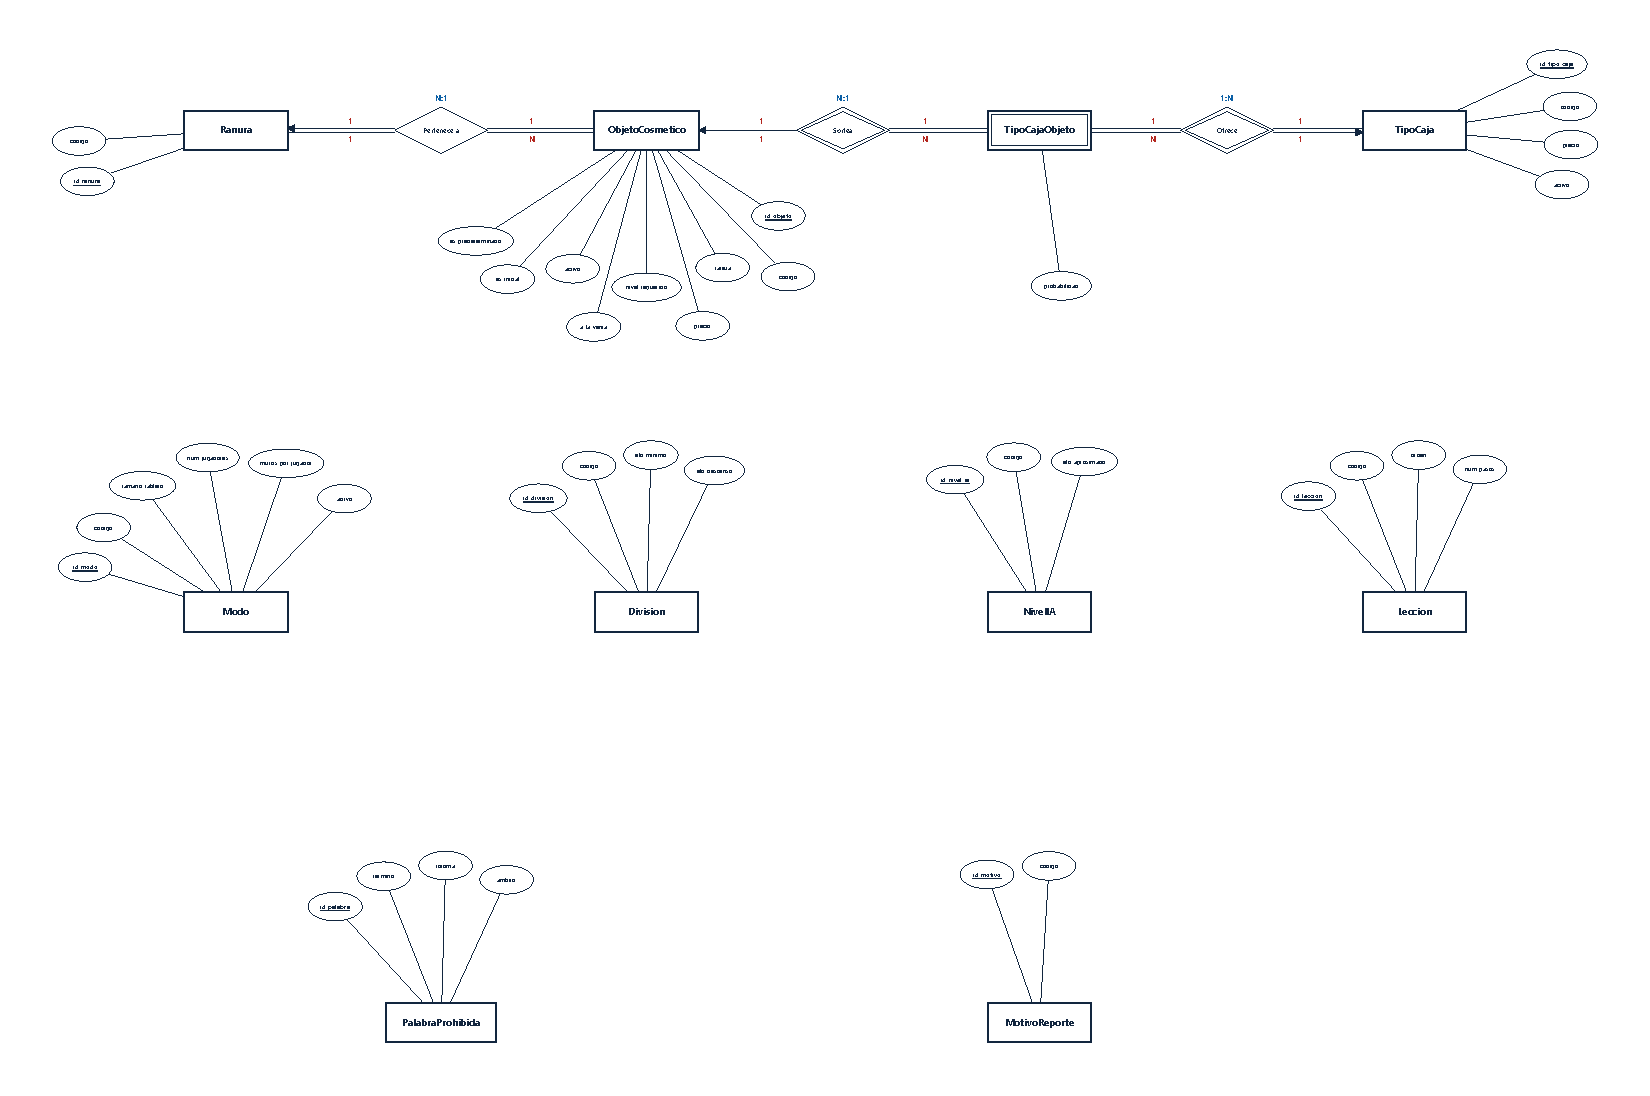
\includegraphics[width=\linewidth,height=0.8\textheight,keepaspectratio]{er/salida/catalogos}
\end{center}
\end{landscape}

\clearpage
\subsubsection*{Cuenta y acceso}
\addcontentsline{toc}{subsubsection}{Diagrama: cuenta y acceso}
\textit{Usuario} con todos sus atributos, y las sesiones, los códigos, los tokens y las aceptaciones de términos que dependen de él.
\begin{center}
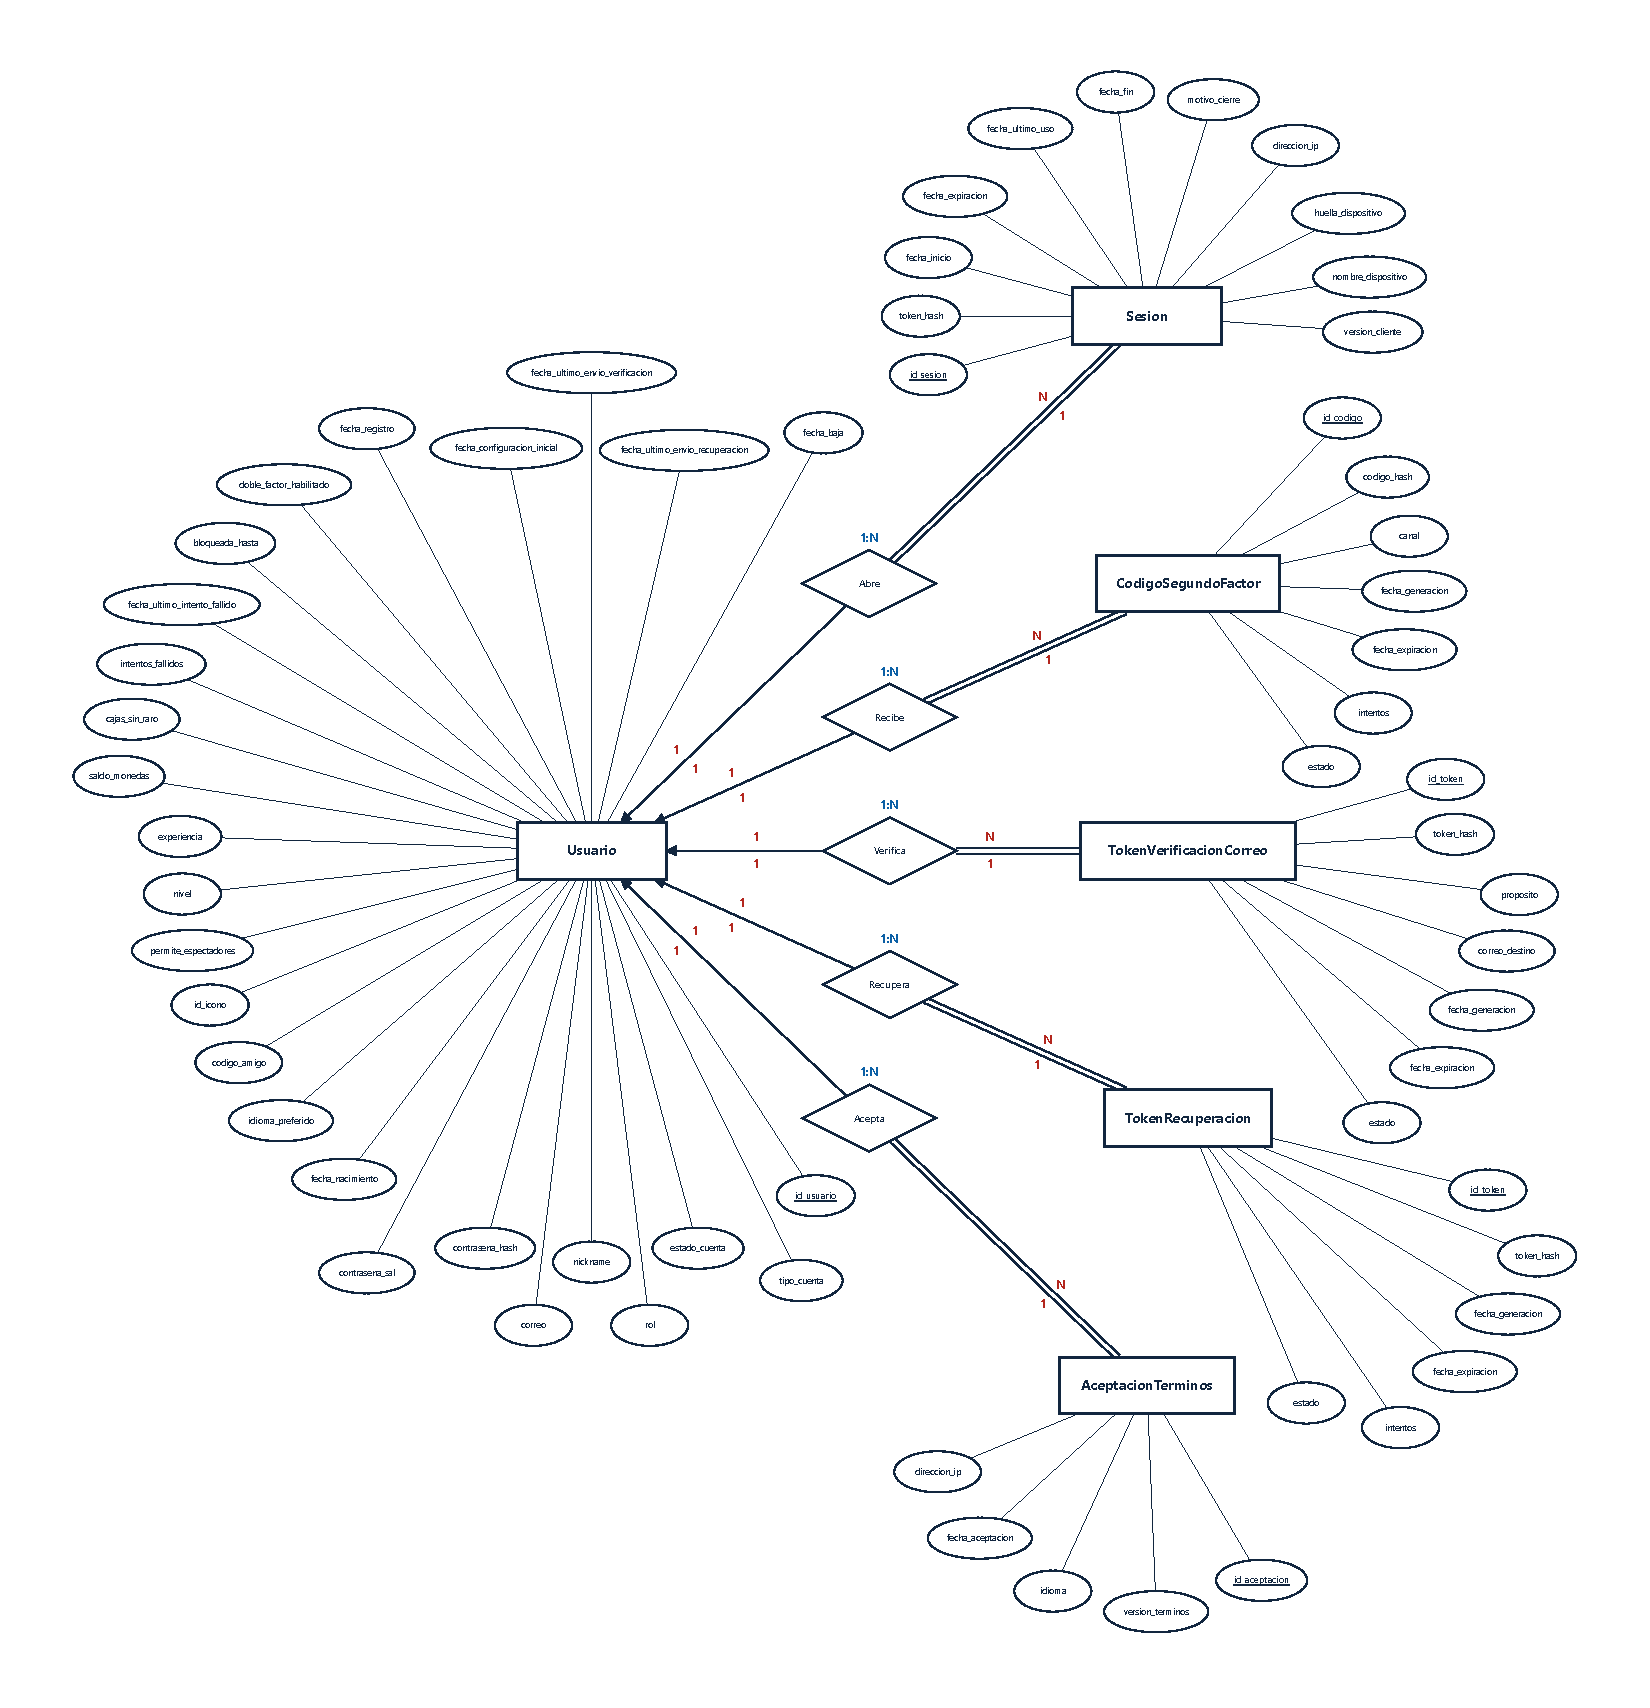
\includegraphics[width=\linewidth,height=0.82\textheight,keepaspectratio]{er/salida/cuenta}
\end{center}

\begin{landscape}
\subsubsection*{Perfil y personalización}
\addcontentsline{toc}{subsubsection}{Diagrama: perfil y personalización}
El perfil público y los objetos cosméticos: lo que el jugador posee (\textit{UsuarioObjeto}) y lo que lleva equipado en cada ranura (\textit{Equipamiento}), que solo puede ser algo que posee.
\begin{center}
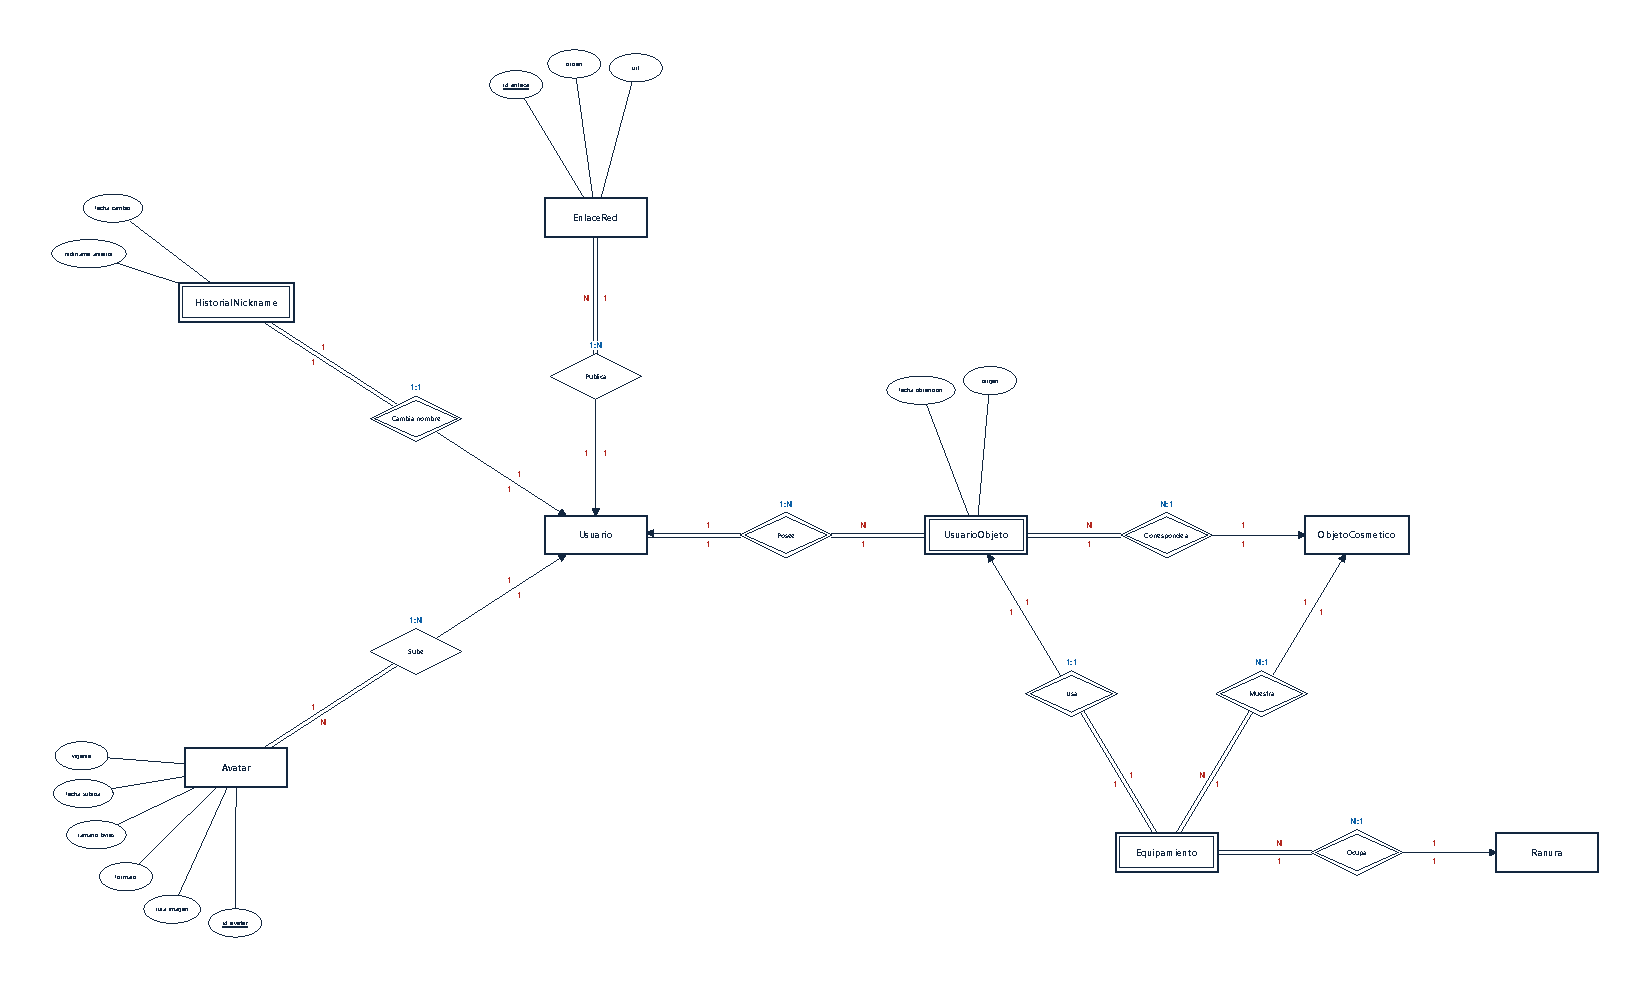
\includegraphics[width=\linewidth,height=0.8\textheight,keepaspectratio]{er/salida/perfil}
\end{center}
\end{landscape}

\begin{landscape}
\subsubsection*{Partida}
\addcontentsline{toc}{subsubsection}{Diagrama: partida}
La partida y la participación de cada jugador, con las jugadas, las ofertas de tablas, los enlaces de espectador y el aspecto fijado al empezar. El ganador no es una relación aparte: es la participación con resultado \at{GANADA}.
\begin{center}
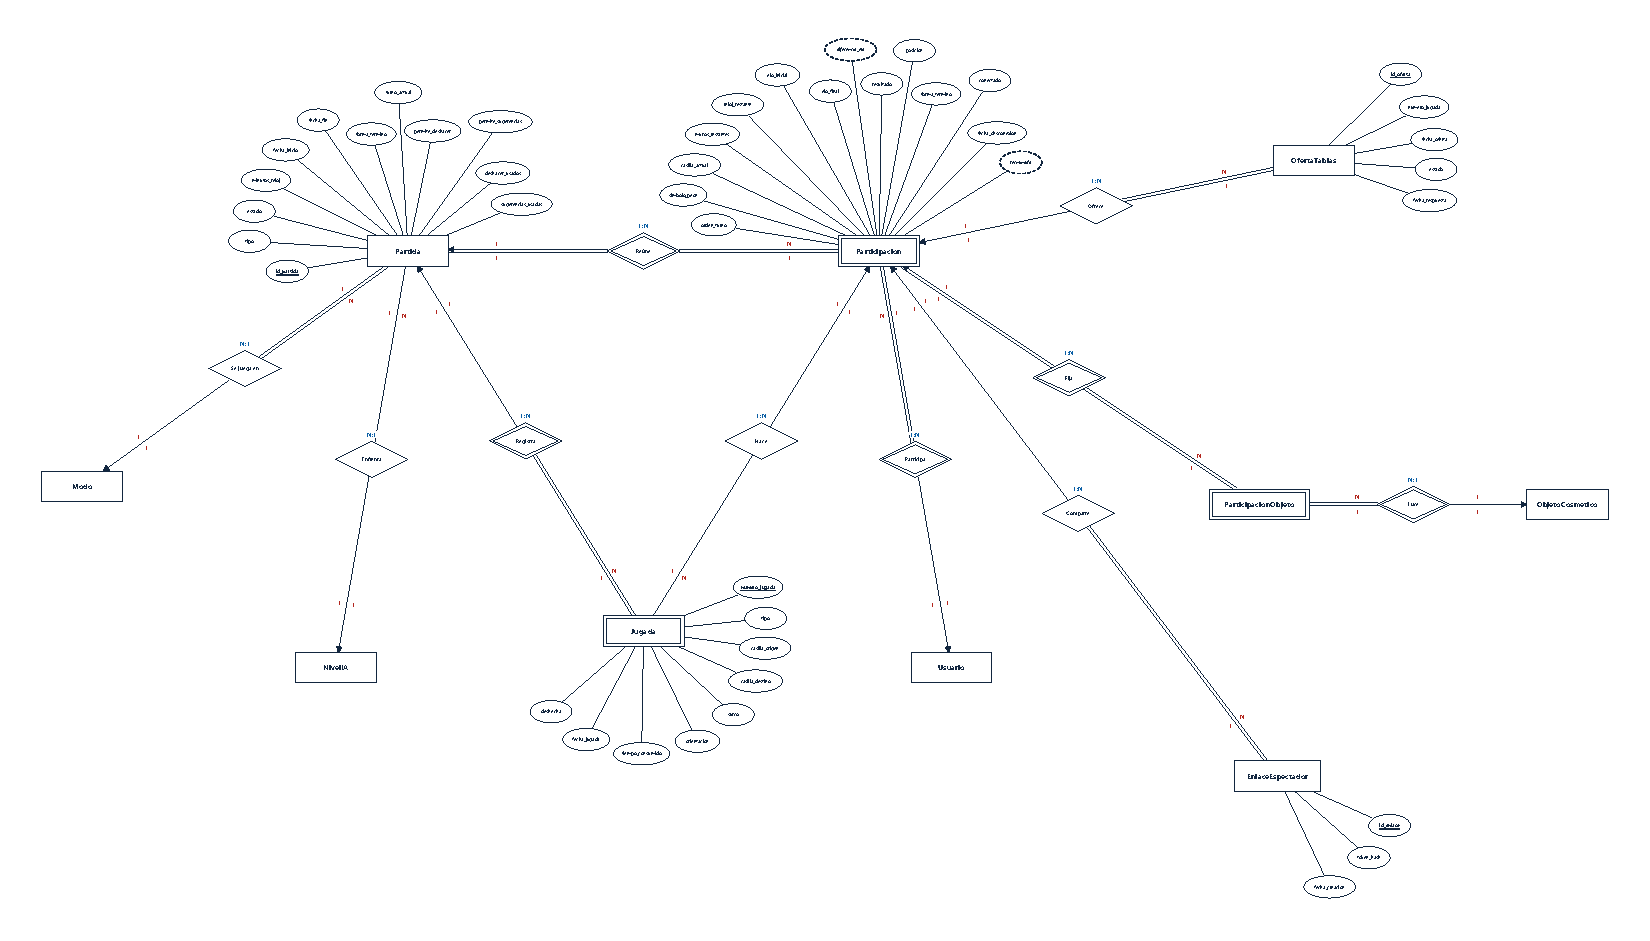
\includegraphics[width=\linewidth,height=0.8\textheight,keepaspectratio]{er/salida/partida}
\end{center}
\end{landscape}

\clearpage
\subsubsection*{Emparejamiento, salas y chat}
\addcontentsline{toc}{subsubsection}{Diagrama: emparejamiento, salas y chat}
La cola clasificatoria, las salas privadas con sus plazas e invitaciones, y los mensajes, que pertenecen a una partida, a una sala o a un canal general.
\begin{center}
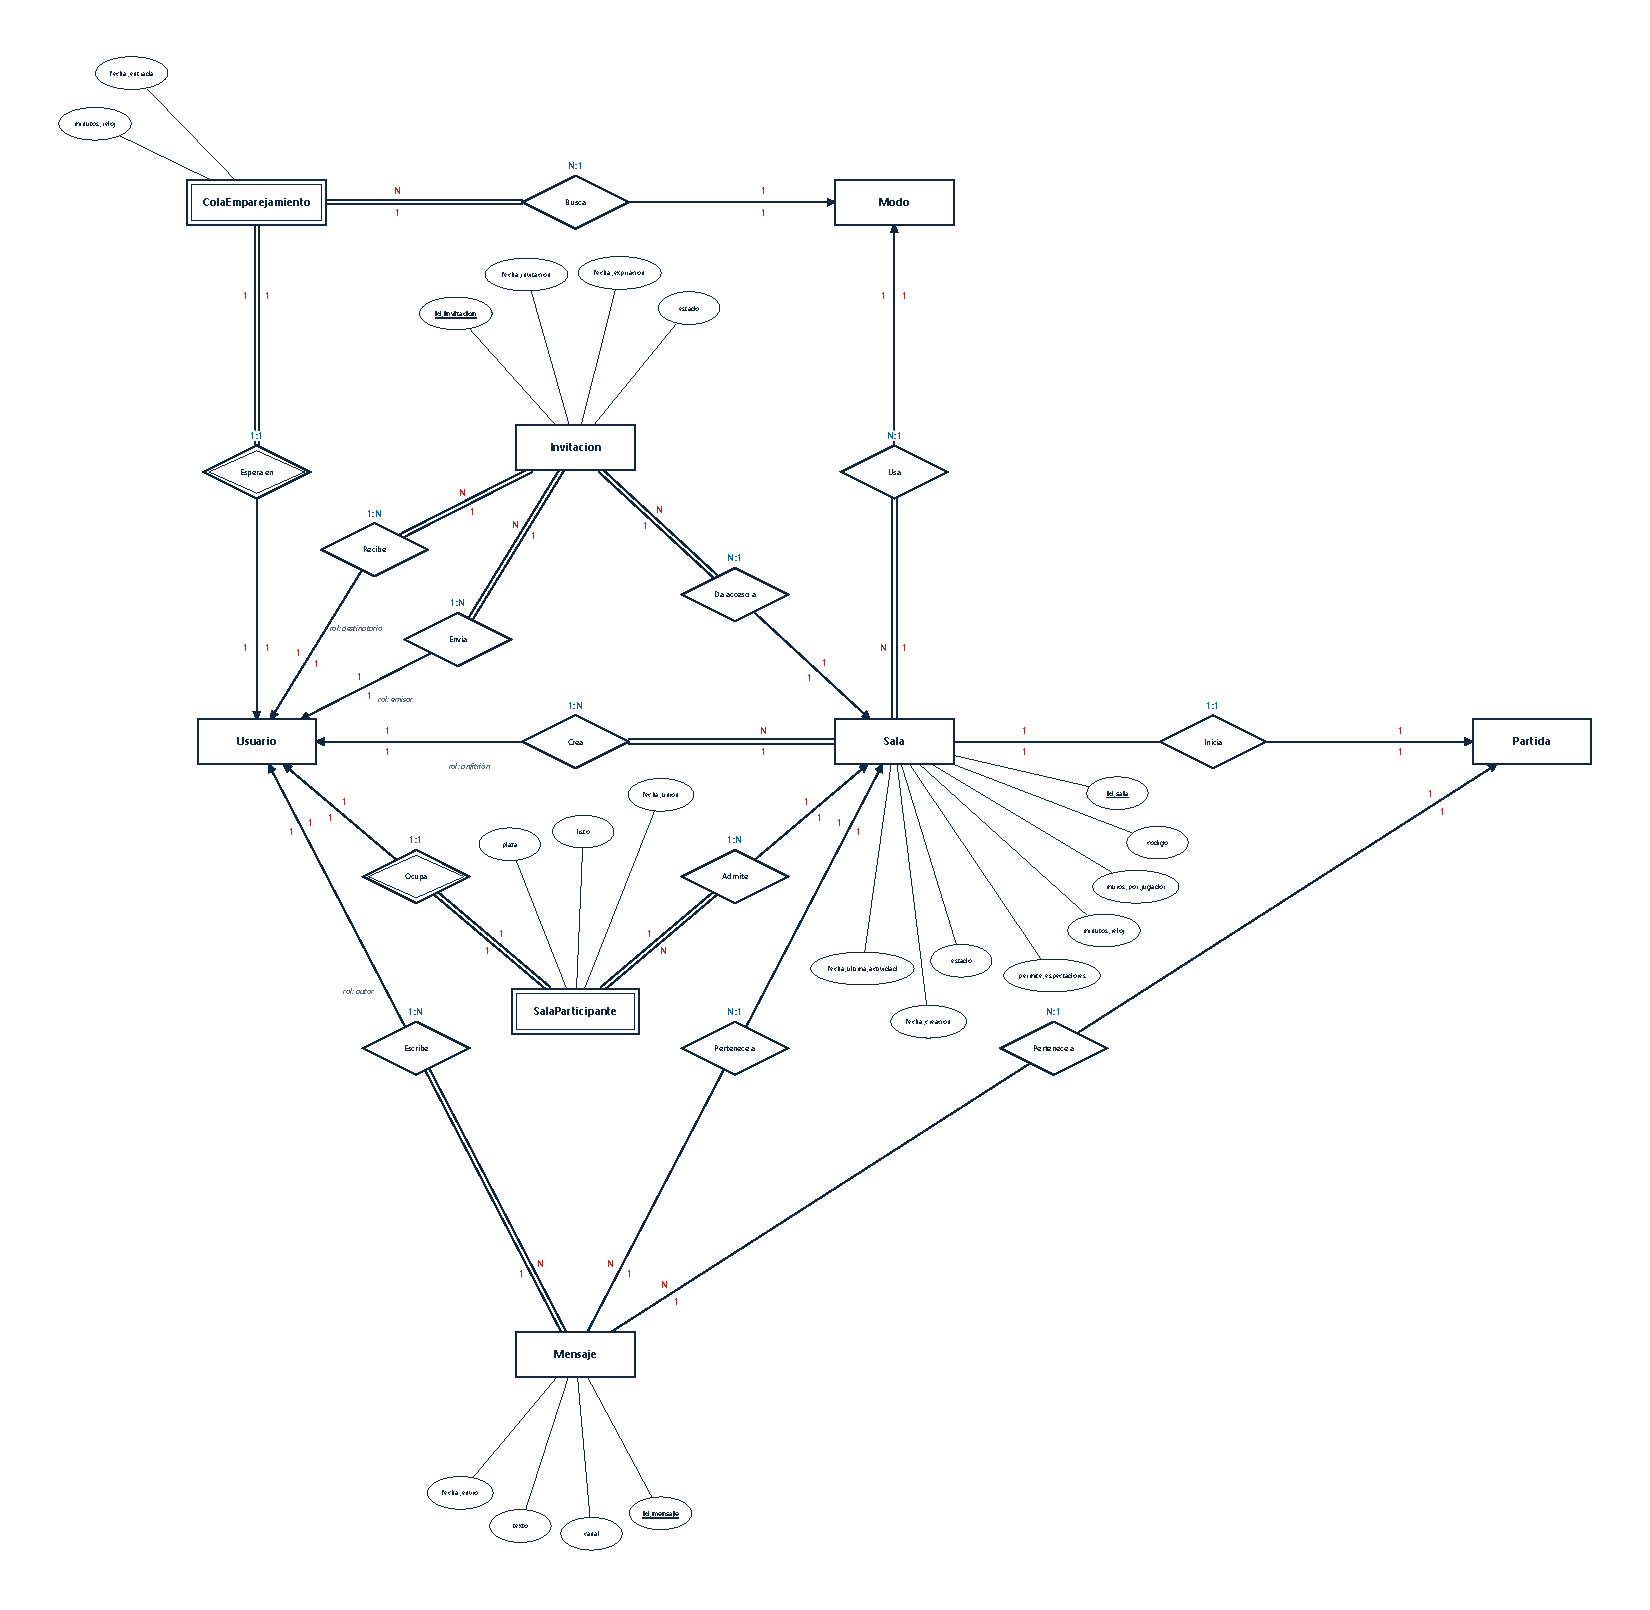
\includegraphics[width=\linewidth,height=0.82\textheight,keepaspectratio]{er/salida/salas}
\end{center}

\begin{landscape}
\subsubsection*{Clasificación y economía}
\addcontentsline{toc}{subsubsection}{Diagrama: clasificación y economía}
A la izquierda, las estadísticas por modo y los cambios de división; a la derecha, las cajas, su contenido y los movimientos de monedas.
\begin{center}
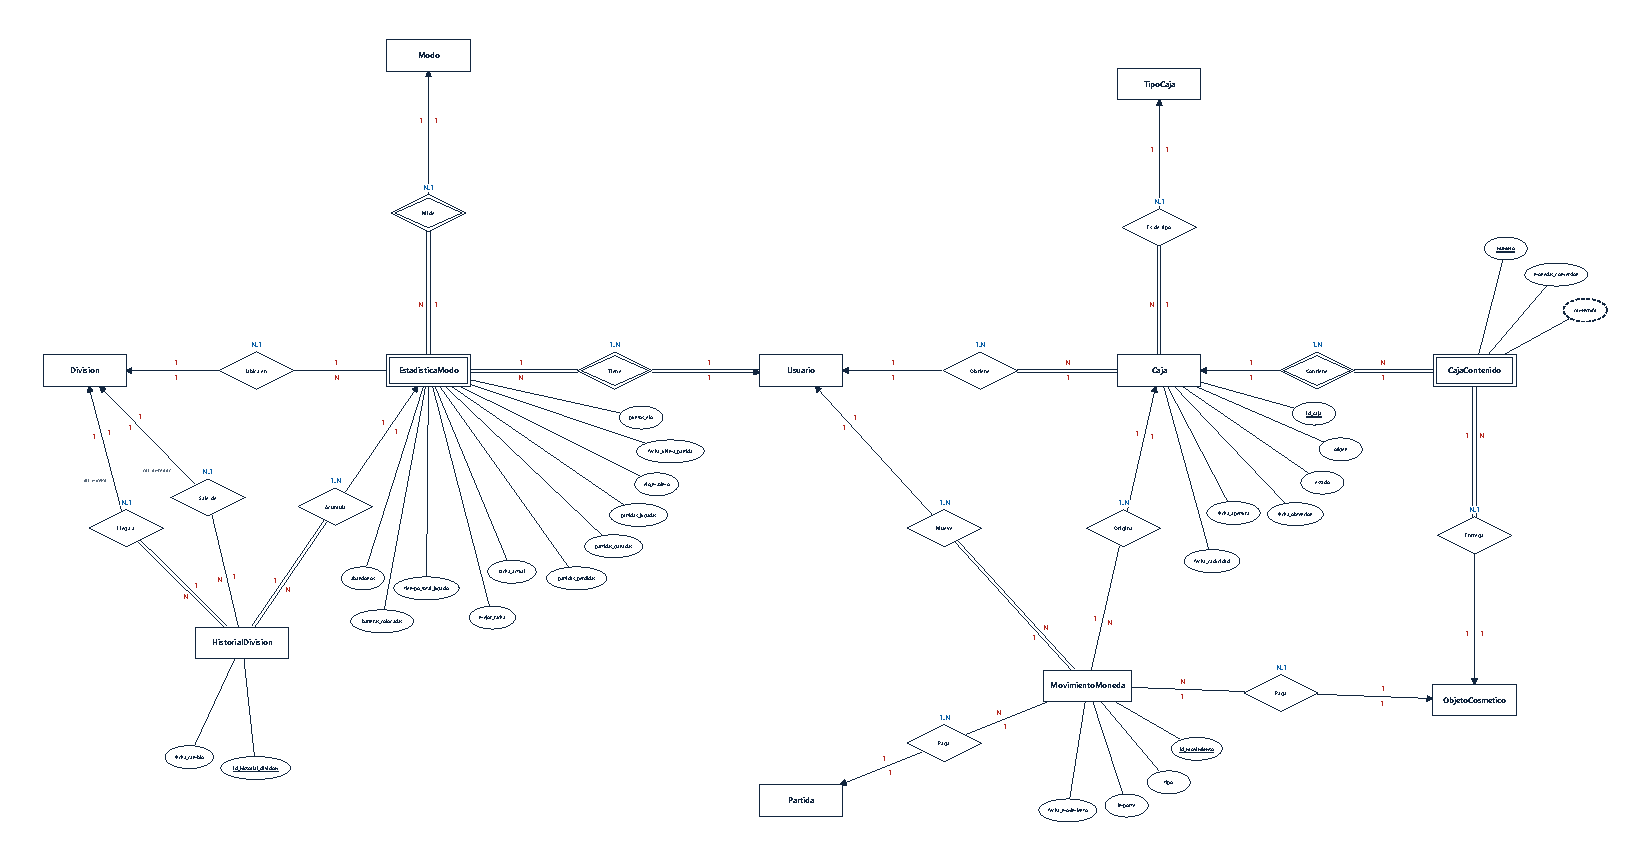
\includegraphics[width=\linewidth,height=0.8\textheight,keepaspectratio]{er/salida/economia}
\end{center}
\end{landscape}

\clearpage
\subsubsection*{Relaciones entre jugadores y tutorial}
\addcontentsline{toc}{subsubsection}{Diagrama: relaciones entre jugadores y tutorial}
Amistades, solicitudes, silencios y bloqueos, cada uno con dos relaciones hacia \textit{Usuario}, una por papel, y el avance de cada jugador en las lecciones del tutorial.
\begin{center}
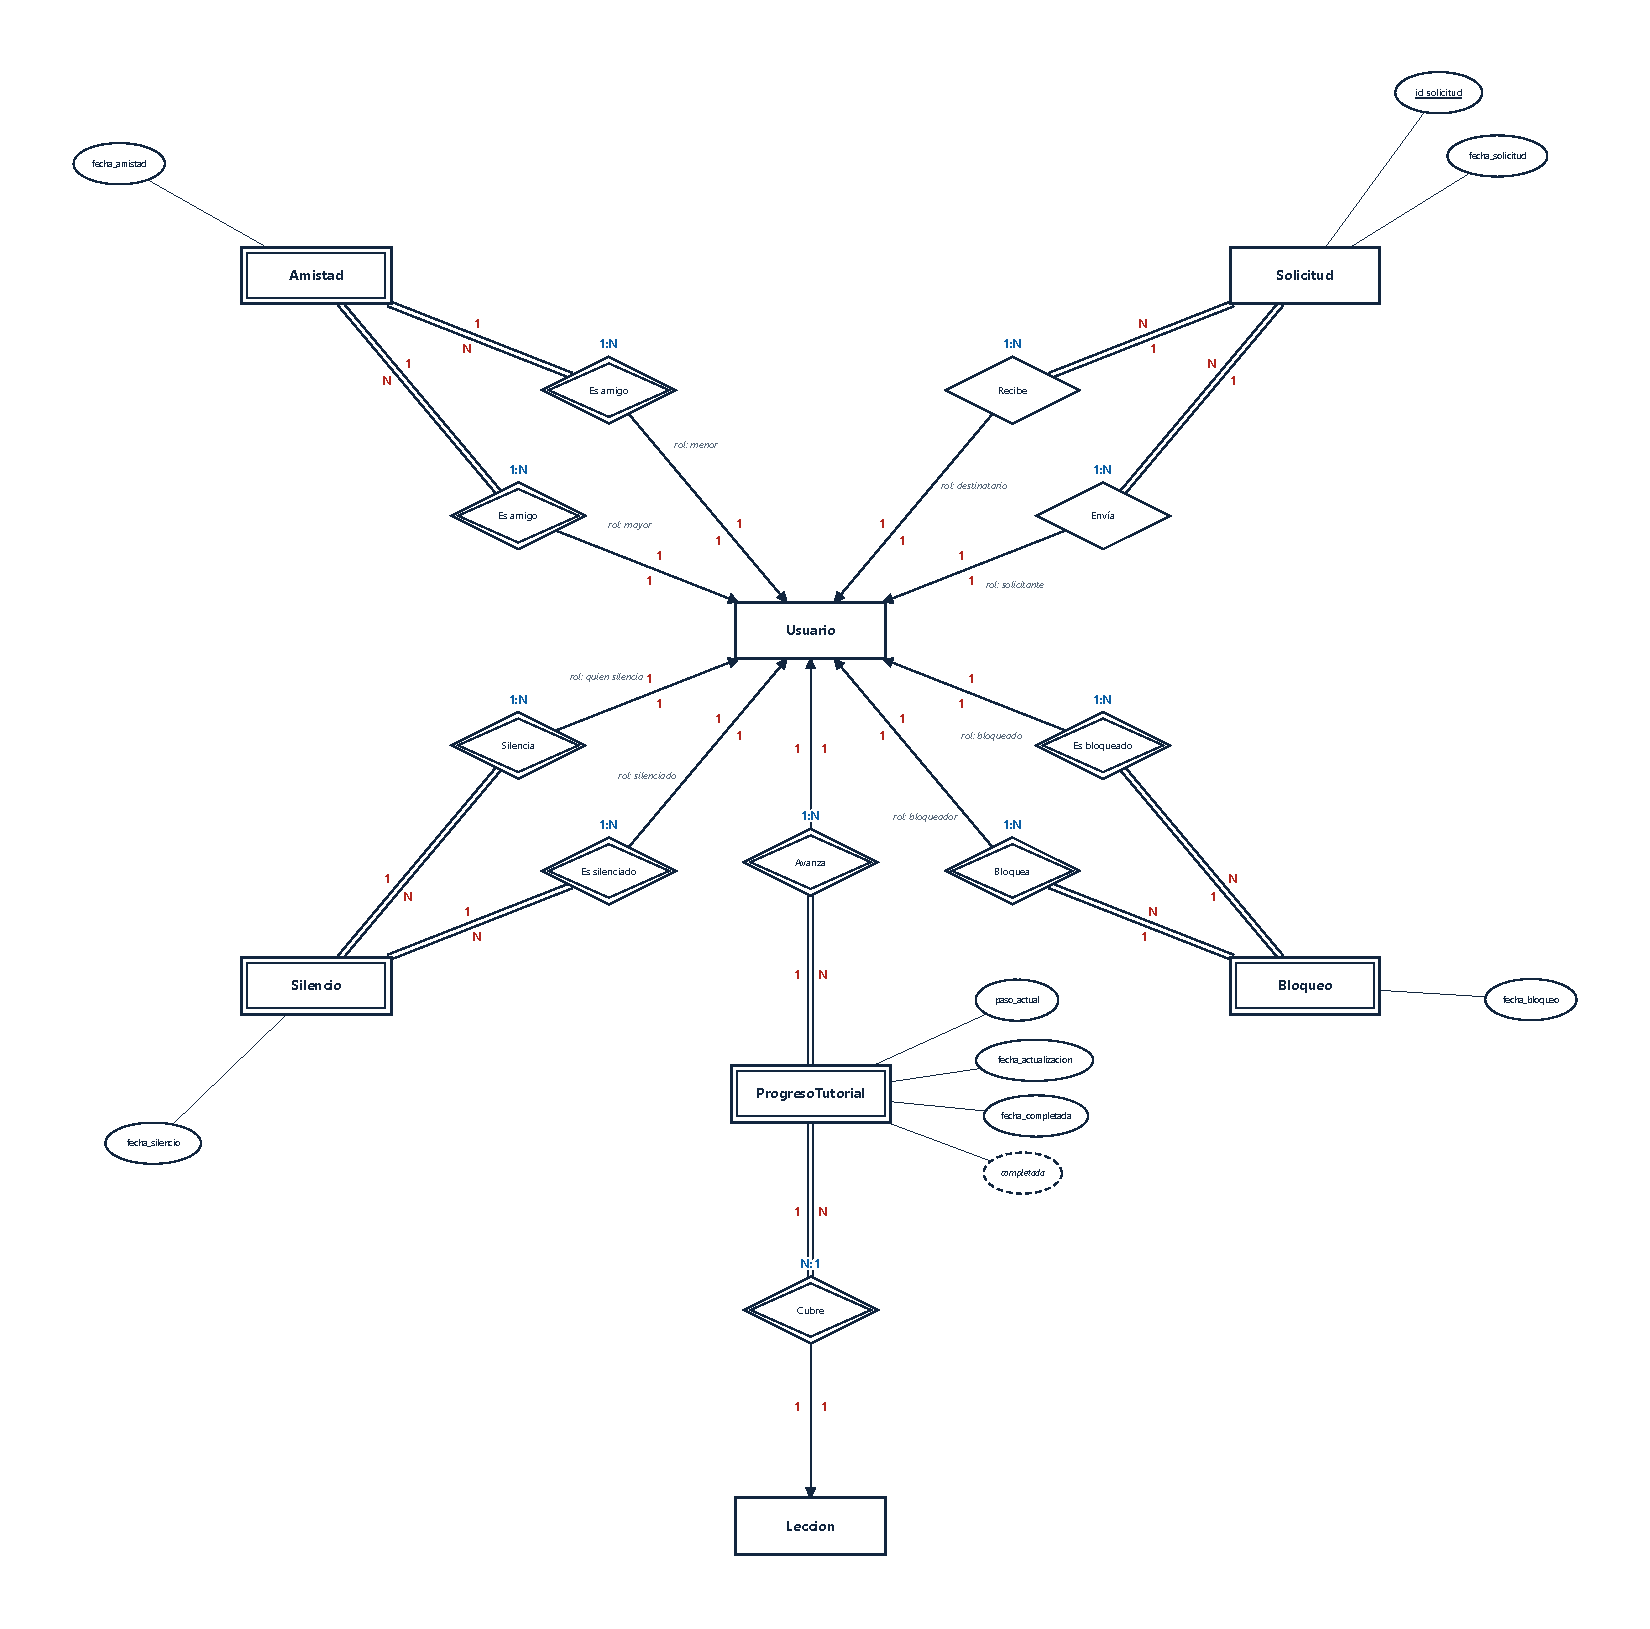
\includegraphics[width=\linewidth,height=0.82\textheight,keepaspectratio]{er/salida/social}
\end{center}

\clearpage
\subsubsection*{Moderación y bitácoras}
\addcontentsline{toc}{subsubsection}{Diagrama: moderación y bitácoras}
Reportes, sanciones, apelaciones y las dos bitácoras. El reporte se relaciona dos veces con \textit{Participacion} porque la partida adjunta tuvo que jugarla tanto el reportante como el reportado (\mbox{CU-42} \mbox{RN-09}).
\begin{center}
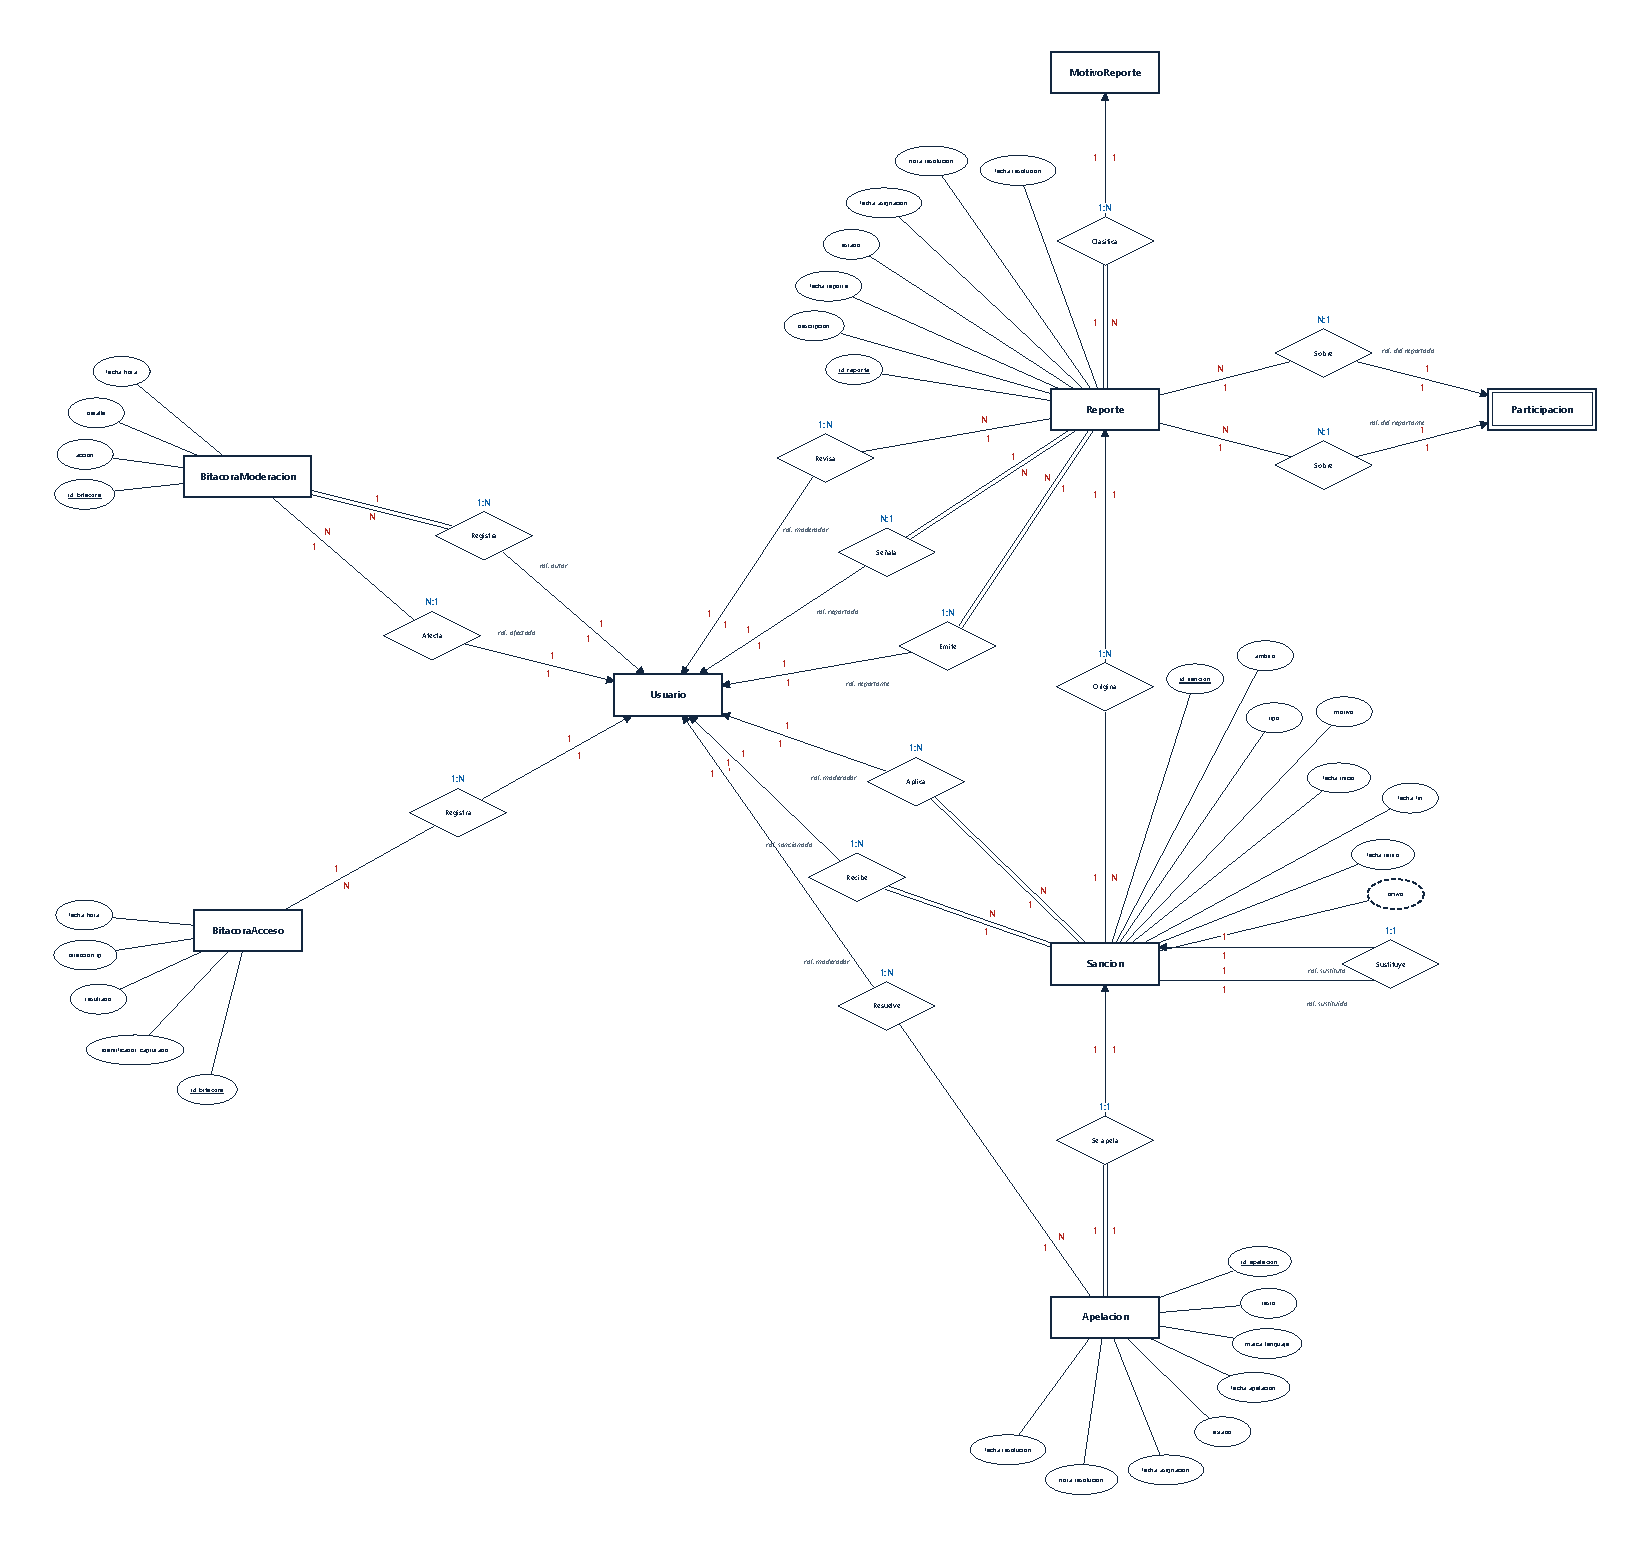
\includegraphics[width=\linewidth,height=0.82\textheight,keepaspectratio]{er/salida/moderacion}
\end{center}
\clearpage

%=====================================================================
% Modelo de datos · Identificación de entidades
%=====================================================================
\subsection*{Identificación de entidades}
\addcontentsline{toc}{subsection}{Identificación de entidades}

Una estructura es entidad del modelo si algún caso de uso la escribe, o si es un catálogo que los casos de uso leen y que se carga por SQL (\mbox{D-09}). Es el mismo criterio de la Matriz 1: ninguna tabla queda sin un caso que la justifique. Tampoco al revés: los datos que se calculan al consultarse —el historial de elo, el marcador entre dos jugadores, la duración de una partida— y los que viven solo en la memoria del servidor —los espectadores y los emotes (\mbox{D-10}, \mbox{D-19})— no son entidades.

Cada entidad se clasifica según cómo se identifica:

\begin{reglas}
  \item \textbf{Fuerte.} Tiene identidad propia, con una llave sustituta, aunque dependa de otra entidad por una llave foránea obligatoria.
  \item \textbf{Débil.} Se identifica por la llave de la entidad de la que depende más un discriminador propio, como el número de jugada dentro de la partida.
  \item \textbf{Dependiente (1:0..1).} Su llave es la misma llave foránea: existe a lo sumo una por cada fila de la entidad de la que depende.
  \item \textbf{Asociativa (N:M).} Resuelve una relación de muchos a muchos; su llave está formada por las llaves de las entidades que relaciona.
  \item \textbf{Catálogo.} Datos de referencia que se cargan por SQL y que ningún caso de uso modifica.
\end{reglas}

% Archivo generado por bd/generar_tablas.ps1 a partir de bd/bastion.sql. No editar a mano.
\begin{center}\small
\begin{longtable}{|L{0.24\textwidth}|L{0.17\textwidth}|L{0.49\textwidth}|}
\hline
\textbf{Entidad} & \textbf{Clase} & \textbf{Qué representa} \\ \hline
\endfirsthead
\hline
\textbf{Entidad} & \textbf{Clase} & \textbf{Qué representa} \\ \hline
\endhead
\multicolumn{3}{|l|}{\textbf{Catálogos precargados (\mbox{D-09})}} \\ \hline
\textit{Ranura} & Catálogo & Catálogo de las seis ranuras de personalización: peón, muro, tablero, título, marco y emotes (\mbox{D-03}). \\ \hline
\textit{Objeto\-Cosmetico} & Catálogo & Catálogo de objetos cosméticos. Cada objeto pertenece a una sola ranura (\mbox{D-03}). \\ \hline
\textit{Modo} & Catálogo & Catálogo de modos de juego; cada modo fija tablero, jugadores y muros (\mbox{D-04}). \\ \hline
\textit{Division} & Catálogo & Catálogo de divisiones del ranking con sus umbrales de ascenso y descenso. \\ \hline
\textit{Nivel\-IA} & Catálogo & Catálogo de los cuatro niveles de la IA (\mbox{CU-27} \mbox{RN-02}). \\ \hline
\textit{Leccion} & Catálogo & Catálogo de las siete lecciones del tutorial (\mbox{CU-41} \mbox{RN-01}). \\ \hline
\textit{Tipo\-Caja} & Catálogo & Catálogo de tipos de caja que se venden o se otorgan (\mbox{CU-39}). \\ \hline
\textit{Tipo\-Caja\-Objeto} & Catálogo asociativo & Objetos que puede contener cada tipo de caja y su probabilidad; es la relación N:M entre TipoCaja y ObjetoCosmetico. \\ \hline
\textit{Palabra\-Prohibida} & Catálogo & Catálogo del filtro de palabras que se aplica en el servidor al nickname y al chat (\mbox{CON-09}). \\ \hline
\textit{Motivo\-Reporte} & Catálogo & Catálogo de los cinco motivos de reporte (\mbox{CU-42} \mbox{RN-08}). \\ \hline
\multicolumn{3}{|l|}{\textbf{Cuenta y acceso}} \\ \hline
\textit{Usuario} & Fuerte & Cuenta de un jugador, invitado, moderador o administrador. Es la entidad central: casi todas las demás dependen de ella y su fila nunca se borra (\mbox{D-07}, \mbox{D-17}). \\ \hline
\textit{Sesion} & Fuerte & Sesión abierta desde un dispositivo. Una cuenta puede tener varias a la vez (\mbox{D-01}); al cerrarse no se borra. \\ \hline
\textit{Codigo\-Segundo\-Factor} & Fuerte & Código del segundo factor emitido en un inicio de sesión (\mbox{CU-01} \mbox{RN-08}, \mbox{RN-09}). \\ \hline
\textit{Token\-Verificacion\-Correo} & Fuerte & Token del enlace que verifica el correo del alta o confirma un cambio de correo (\mbox{CU-04}, \mbox{D-20}). \\ \hline
\textit{Token\-Recuperacion} & Fuerte & Código enviado por correo para recuperar la contraseña (\mbox{CU-03}). \\ \hline
\textit{Aceptacion\-Terminos} & Fuerte & Registro de la versión de los términos de uso que aceptó cada cuenta (\mbox{CU-02} \mbox{RN-12}). \\ \hline
\multicolumn{3}{|l|}{\textbf{Perfil y personalización}} \\ \hline
\textit{Historial\-Nickname} & Dependiente (1:0..1) & Cambio de nombre de una cuenta, para que un jugador reportado no se vuelva irreconocible (\mbox{CU-13} \mbox{RN-03}). \\ \hline
\textit{Avatar} & Fuerte & Imagen subida por el jugador como foto de perfil (\mbox{CU-12} \mbox{FA-01}). \\ \hline
\textit{Enlace\-Red} & Fuerte & Enlace a una red social que el jugador muestra en su perfil (\mbox{CU-12}). \\ \hline
\textit{Usuario\-Objeto} & Asociativa (N:M) & Objetos cosméticos que posee cada cuenta; es la relación N:M entre Usuario y ObjetoCosmetico (relación Posee del diagrama). \\ \hline
\textit{Equipamiento} & Asociativa (N:M) & Objeto que cada cuenta lleva equipado en cada ranura; siempre hay exactamente uno por ranura (\mbox{CU-14} \mbox{RN-01}). \\ \hline
\multicolumn{3}{|l|}{\textbf{Partida}} \\ \hline
\textit{Partida} & Dependiente (1:0..1) & Partida clasificatoria, privada o contra la IA. Se guarda completa porque de ella dependen el historial, la repetición, la reconexión y los reportes. \\ \hline
\textit{Participacion} & Asociativa (N:M) & Participación de un jugador en una partida; es la relación N:M entre Usuario y Partida (relación Participa del diagrama). La IA no tiene participación (\mbox{D-12}). \\ \hline
\textit{Participacion\-Objeto} & Asociativa (N:M) & Aspecto con el que cada jugador entró a la partida, una fila por ranura; no cambia aunque el jugador equipe otra cosa (\mbox{CU-14} \mbox{RN-03}, \mbox{CU-37} \mbox{RN-03}). \\ \hline
\textit{Jugada} & Débil & Movimiento de peón o colocación de muro, en orden. El tablero se reconstruye sumando las jugadas; los muros no tienen tabla propia (\mbox{CU-21}). \\ \hline
\textit{Oferta\-Tablas} & Fuerte & Oferta de tablas en una partida de dos jugadores (\mbox{CU-22}). Se guarda para la reconexión y como prueba de acoso. \\ \hline
\textit{Enlace\-Espectador} & Fuerte & Enlace compartido para ver una partida desde fuera del juego. Es lo único que se guarda de los espectadores (\mbox{D-19}). \\ \hline
\multicolumn{3}{|l|}{\textbf{Emparejamiento, salas y chat}} \\ \hline
\textit{Cola\-Emparejamiento} & Dependiente (1:0..1) & Jugadores que esperan partida clasificatoria. Se persiste para poder vaciarla y avisar si el servidor se reinicia (\mbox{CU-17}). \\ \hline
\textit{Sala} & Fuerte & Sala privada con código, con los ajustes que elige el anfitrión (\mbox{CU-18}). \\ \hline
\textit{Sala\-Participante} & Dependiente (1:0..1) & Plaza que ocupa un jugador en una sala. Describe un estado presente y se borra al salir (\mbox{CU-19}). \\ \hline
\textit{Invitacion} & Fuerte & Invitación a jugar, que da acceso a una sala sin conocer su código (\mbox{CU-32}). \\ \hline
\textit{Mensaje} & Fuerte & Mensaje de chat. Se guarda porque el reporte lo adjunta como prueba (\mbox{CU-28}, \mbox{CU-42}). \\ \hline
\multicolumn{3}{|l|}{\textbf{Clasificación y economía}} \\ \hline
\textit{Estadistica\-Modo} & Asociativa (N:M) & Estadísticas y elo de cada cuenta en cada modo; es la relación N:M entre Usuario y Modo (relación Tiene del diagrama, ahora por modo, \mbox{D-04}). \\ \hline
\textit{Historial\-Division} & Fuerte & Cambio de división de una cuenta en un modo. No se deduce de una sola partida por las partidas de margen, así que se guarda (\mbox{CU-15}). \\ \hline
\textit{Caja} & Fuerte & Caja comprada u obtenida al subir de nivel. Existe sin abrir entre la compra y la apertura (\mbox{CU-39} \mbox{RN-09}). \\ \hline
\textit{Caja\-Contenido} & Débil & Los tres objetos que salieron al abrir una caja, registrados para poder comprobarlos después (\mbox{CU-39} \mbox{RN-07}). \\ \hline
\textit{Movimiento\-Moneda} & Fuerte & Entrada o salida de monedas. El saldo verdadero es su suma; nunca se modifica ni se elimina (\mbox{CU-40} \mbox{RN-01}). \\ \hline
\multicolumn{3}{|l|}{\textbf{Relaciones entre jugadores y tutorial}} \\ \hline
\textit{Amistad} & Asociativa (N:M) & Amistad recíproca entre dos cuentas, guardada una sola vez por par ordenado (\mbox{CU-31} \mbox{RN-03}). \\ \hline
\textit{Solicitud} & Fuerte & Solicitud de amistad pendiente. Tiene dirección, a diferencia de la amistad, y se borra al responderse (\mbox{CU-30}, \mbox{CU-31}). \\ \hline
\textit{Silencio} & Asociativa (N:M) & Jugador silenciado por otro; solo lo consulta quien silenció (\mbox{CU-33}). \\ \hline
\textit{Bloqueo} & Asociativa (N:M) & Bloqueo entre dos jugadores; impide emparejar, invitar, buscar, solicitar y compartir sala (\mbox{CU-33} \mbox{RN-05}). \\ \hline
\textit{Progreso\-Tutorial} & Asociativa (N:M) & Avance de cada cuenta en cada lección del tutorial; es la relación N:M entre Usuario y Leccion (\mbox{CU-41}). \\ \hline
\multicolumn{3}{|l|}{\textbf{Moderación y bitácoras}} \\ \hline
\textit{Reporte} & Fuerte & Denuncia de un jugador contra otro. Las pruebas se adjuntan por referencia a la partida, no por copia (\mbox{CU-42} \mbox{RN-01}). \\ \hline
\textit{Sancion} & Fuerte & Sanción aplicada por un moderador, de ámbito de cuenta o de chat (\mbox{D-05}). Sustituye al Baneo del diagrama; al retirarse se desactiva, no se borra. \\ \hline
\textit{Apelacion} & Fuerte & Apelación de una sanción por parte del sancionado; hay a lo sumo una por sanción (\mbox{CU-45} \mbox{RN-01}). \\ \hline
\textit{Bitacora\-Moderacion} & Fuerte & Registro de cada acción de moderación y administración, incluida la consulta de las bitácoras (\mbox{CU-48} \mbox{RN-04}). Solo admite inserción. \\ \hline
\textit{Bitacora\-Acceso} & Fuerte & Registro de cada intento de acceso y de cada cambio de credenciales, exitoso o no. Nunca contiene contraseñas ni códigos (\mbox{CU-48} \mbox{RN-05}). \\ \hline
\end{longtable}
\end{center}


%=====================================================================
% Modelo de datos · Atributos de cada entidad
%=====================================================================
\subsection*{Atributos de cada entidad}
\addcontentsline{toc}{subsection}{Atributos de cada entidad}

Cada tabla lista los atributos de una entidad con su tipo en SQL Server, si admiten nulo y si forman parte de una llave: \textbf{PK} para la llave primaria, \textbf{FK} para una llave foránea y \textbf{UQ} para un atributo único por sí solo. Las llaves compuestas y las restricciones de unicidad con condición se detallan en las secciones siguientes.

Un atributo sin tipo de almacenamiento, marcado como \emph{calculada}, es una columna calculada no persistida: la base la obtiene de otras columnas de la misma fila cada vez que se lee y no la guarda. Se usa para los cuatro atributos que los casos de uso nombran pero que dependen de otros atributos de la fila; así la aplicación los lee con el nombre de siempre y la tabla sigue en tercera forma normal.

% Archivo generado por bd/generar_tablas.ps1 a partir de bd/crear_tablas.sql. No editar a mano.
% Archivo generado por bd/generar_tablas.ps1 a partir de bd/crear_tablas.sql. No editar a mano.
\subsubsection*{
Catálogos precargados (\mbox{D-09})
}
\addcontentsline{toc}{subsubsection}{
Catálogos precargados (\mbox{D-09})
}

\atributosde{Ranura}{Catálogo de las seis ranuras de personalización: peón, muro, tablero, título, marco y emotes (\mbox{D-03}).}
\begin{tablaatributos}
\texttt{id\_\allowbreak{}ranura} & \texttt{TINYINT} & No & PK & Identificador de la ranura. \\ \hline
\texttt{codigo} & \texttt{VARCHAR(20)} & No & UQ & Clave de la ranura en los diccionarios de recursos (\mbox{D-21}): \texttt{PEON}, \texttt{MURO}, \texttt{TABLERO}, \texttt{TITULO}, \texttt{MARCO} o \texttt{EMOTES}. Sin CHECK: añadir una ranura es insertar una fila (\mbox{CU-14}). \\ \hline
\end{tablaatributos}

\atributosde{ObjetoCosmetico}{Catálogo de objetos cosméticos. Cada objeto pertenece a una sola ranura (\mbox{D-03}).}
\begin{tablaatributos}
\texttt{id\_\allowbreak{}objeto} & \texttt{INT} & No & PK & Identificador del objeto. \\ \hline
\texttt{id\_\allowbreak{}ranura} & \texttt{TINYINT} & No & FK & Ranura en la que se equipa. \\ \hline
\texttt{codigo} & \texttt{VARCHAR(40)} & No & UQ & Clave del objeto en los diccionarios de recursos, como \texttt{PEON\_\allowbreak{}CLASICO}; con ella el cliente muestra su nombre en el idioma del usuario (\mbox{D-21}). \\ \hline
\texttt{rareza} & \texttt{VARCHAR(10)} & No &  & \texttt{COMUN}, \texttt{RARO}, \texttt{EPICO} o \texttt{LEGENDARIO}. \\ \hline
\texttt{precio} & \texttt{INT} & No &  & Precio en monedas del juego; el válido es este y no el del cliente (\mbox{CU-38} \mbox{RN-03}). Por omisión, \texttt{0}. \\ \hline
\texttt{nivel\_\allowbreak{}requerido} & \texttt{SMALLINT} & No &  & Nivel mínimo para comprarlo (\mbox{CU-38} \mbox{RN-04}). Por omisión, \texttt{1}. \\ \hline
\texttt{a\_\allowbreak{}la\_\allowbreak{}venta} & \texttt{BIT} & No &  & Si se ofrece en la tienda. Por omisión, \texttt{0}. \\ \hline
\texttt{activo} & \texttt{BIT} & No &  & En falso, retirado del catálogo; quien lo tiene equipado lo conserva (\mbox{CU-14} \mbox{RN-04}). Por omisión, \texttt{1}. \\ \hline
\texttt{es\_\allowbreak{}inicial} & \texttt{BIT} & No &  & Se otorga al dar de alta la cuenta. Por omisión, \texttt{0}. \\ \hline
\texttt{es\_\allowbreak{}predeterminado} & \texttt{BIT} & No &  & Se equipa al dar de alta; exactamente uno por ranura. Por omisión, \texttt{0}. \\ \hline
\end{tablaatributos}

\atributosde{Modo}{Catálogo de modos de juego; cada modo fija tablero, jugadores y muros (\mbox{D-04}).}
\begin{tablaatributos}
\texttt{id\_\allowbreak{}modo} & \texttt{TINYINT} & No & PK & Identificador del modo. \\ \hline
\texttt{codigo} & \texttt{VARCHAR(40)} & No & UQ & Clave del modo en los diccionarios de recursos (\mbox{D-21}): \texttt{CLASICO}, \texttt{CUATRO\_\allowbreak{}JUGADORES} o \texttt{RAPIDA}. \\ \hline
\texttt{tamano\_\allowbreak{}tablero} & \texttt{TINYINT} & No &  & Casillas por lado: 7 o 9. \\ \hline
\texttt{num\_\allowbreak{}jugadores} & \texttt{TINYINT} & No &  & Plazas de la partida: 2 o 4 (\mbox{CU-17} \mbox{RN-02}). \\ \hline
\texttt{muros\_\allowbreak{}por\_\allowbreak{}jugador} & \texttt{TINYINT} & No &  & Muros de cada jugador: 10, 5 o 6 (\mbox{CU-21} \mbox{RN-02}). \\ \hline
\texttt{activo} & \texttt{BIT} & No &  & Solo los modos activos reciben estadísticas al dar de alta (\mbox{CU-02}). Por omisión, \texttt{1}. \\ \hline
\end{tablaatributos}

\atributosde{Division}{Catálogo de divisiones del ranking con sus umbrales de ascenso y descenso.}
\begin{tablaatributos}
\texttt{id\_\allowbreak{}division} & \texttt{TINYINT} & No & PK & Identificador de la división. \\ \hline
\texttt{codigo} & \texttt{VARCHAR(40)} & No & UQ & Clave de la división en los diccionarios de recursos (\mbox{D-21}), como \texttt{BRONCE} o \texttt{MURO\_\allowbreak{}PIEDRA}. \\ \hline
\texttt{elo\_\allowbreak{}minimo} & \texttt{SMALLINT} & No & UQ & Elo con el que se asciende a esta división; ordena las divisiones de la más baja a la más alta. \\ \hline
\texttt{elo\_\allowbreak{}descenso} & \texttt{SMALLINT} & No &  & Elo por debajo del cual se desciende; es el umbral visible (\mbox{CU-25} \mbox{RN-07}). \\ \hline
\end{tablaatributos}

\atributosde{NivelIA}{Catálogo de los cuatro niveles de la IA (\mbox{CU-27} \mbox{RN-02}).}
\begin{tablaatributos}
\texttt{id\_\allowbreak{}nivel\_\allowbreak{}ia} & \texttt{TINYINT} & No & PK & Identificador del nivel. \\ \hline
\texttt{codigo} & \texttt{VARCHAR(40)} & No & UQ & Clave del nivel en los diccionarios de recursos (\mbox{D-21}): \texttt{APRENDIZ}, \texttt{CONSTRUCTOR}, \texttt{ARQUITECTO} o \texttt{BASTION}. \\ \hline
\texttt{elo\_\allowbreak{}aproximado} & \texttt{SMALLINT} & No &  & Fuerza aproximada: 1000, 1500, 1900 o 2300. \\ \hline
\end{tablaatributos}

\atributosde{Leccion}{Catálogo de las siete lecciones del tutorial (\mbox{CU-41} \mbox{RN-01}).}
\begin{tablaatributos}
\texttt{id\_\allowbreak{}leccion} & \texttt{TINYINT} & No & PK & Identificador de la lección. \\ \hline
\texttt{codigo} & \texttt{VARCHAR(40)} & No & UQ & Clave de la lección en los diccionarios de recursos (\mbox{D-21}), como \texttt{MOVER\_\allowbreak{}PEON}; los textos de sus pasos también están en ellos. \\ \hline
\texttt{orden} & \texttt{TINYINT} & No & UQ & Posición en el índice del tutorial. \\ \hline
\texttt{num\_\allowbreak{}pasos} & \texttt{TINYINT} & No &  & Pasos de la lección. \\ \hline
\end{tablaatributos}

\atributosde{TipoCaja}{Catálogo de tipos de caja que se venden o se otorgan (\mbox{CU-39}).}
\begin{tablaatributos}
\texttt{id\_\allowbreak{}tipo\_\allowbreak{}caja} & \texttt{TINYINT} & No & PK & Identificador del tipo de caja. \\ \hline
\texttt{codigo} & \texttt{VARCHAR(40)} & No & UQ & Clave del tipo de caja en los diccionarios de recursos (\mbox{D-21}), como \texttt{CAJA\_\allowbreak{}MADERA}. \\ \hline
\texttt{precio} & \texttt{INT} & No &  & Precio en monedas del juego. \\ \hline
\texttt{activo} & \texttt{BIT} & No &  & En falso, ya no se vende. Por omisión, \texttt{1}. \\ \hline
\end{tablaatributos}

\atributosde{TipoCajaObjeto}{Objetos que puede contener cada tipo de caja y su probabilidad; es la relación N:M entre TipoCaja y ObjetoCosmetico.}
\begin{tablaatributos}
\texttt{id\_\allowbreak{}tipo\_\allowbreak{}caja} & \texttt{TINYINT} & No & PK, FK & Tipo de caja. \\ \hline
\texttt{id\_\allowbreak{}objeto} & \texttt{INT} & No & PK, FK & Objeto que puede salir. \\ \hline
\texttt{probabilidad} & \texttt{DECIMAL(6,3)} & No &  & Porcentaje exacto que se muestra antes de comprar (\mbox{CU-39} \mbox{RN-01}). \\ \hline
\end{tablaatributos}

\atributosde{PalabraProhibida}{Catálogo del filtro de palabras que se aplica en el servidor al nickname y al chat (\mbox{CON-09}).}
\begin{tablaatributos}
\texttt{id\_\allowbreak{}palabra} & \texttt{INT}, identidad & No & PK & Identificador del término. \\ \hline
\texttt{termino} & \texttt{NVARCHAR(100)} & No &  & Término prohibido, con sus eñes y acentos; se compara sin mayúsculas ni acentos. \\ \hline
\texttt{idioma} & \texttt{VARCHAR(10)} & Sí &  & Idioma del término: \texttt{es-MX} o \texttt{en}; nulo si se filtra en todos los idiomas (\mbox{CU-28} \mbox{RN-01}). \\ \hline
\texttt{ambito} & \texttt{VARCHAR(10)} & No &  & \texttt{NICKNAME}, \texttt{CHAT} o \texttt{AMBOS}. \\ \hline
\end{tablaatributos}

\atributosde{MotivoReporte}{Catálogo de los cinco motivos de reporte (\mbox{CU-42} \mbox{RN-08}).}
\begin{tablaatributos}
\texttt{id\_\allowbreak{}motivo} & \texttt{TINYINT} & No & PK & Identificador del motivo. \\ \hline
\texttt{codigo} & \texttt{VARCHAR(40)} & No & UQ & Clave del motivo en los diccionarios de recursos (\mbox{D-21}), como \texttt{LENGUAJE\_\allowbreak{}OFENSIVO}; con ella el cliente muestra su descripción. \\ \hline
\end{tablaatributos}


% Archivo generado por bd/generar_tablas.ps1 a partir de bd/crear_tablas.sql. No editar a mano.
\subsubsection*{
Cuenta y acceso
}
\addcontentsline{toc}{subsubsection}{
Cuenta y acceso
}

\atributosde{Usuario}{Cuenta de un jugador, invitado, moderador o administrador. Es la entidad central: casi todas las demás dependen de ella y su fila nunca se borra (\mbox{D-07}, \mbox{D-17}).}
\begin{tablaatributos}
\texttt{id\_\allowbreak{}usuario} & \texttt{INT}, identidad & No & PK & Identificador de la cuenta; no cambia al vincular un invitado (\mbox{D-02}). \\ \hline
\texttt{tipo\_\allowbreak{}cuenta} & \texttt{VARCHAR(10)} & No &  & \texttt{INVITADO} o \texttt{REGISTRADA}. Discrimina qué credenciales aplican. \\ \hline
\texttt{estado\_\allowbreak{}cuenta} & \texttt{VARCHAR(10)} & No &  & \texttt{PENDIENTE}, \texttt{ACTIVA}, \texttt{SUSPENDIDA}, \texttt{BANEADA} o \texttt{ELIMINADA} (\mbox{CU-01} \mbox{RN-04}). Por omisión, \texttt{PENDIENTE}. \\ \hline
\texttt{rol} & \texttt{VARCHAR(13)} & No &  & \texttt{JUGADOR}, \texttt{MODERADOR} o \texttt{ADMINISTRADOR}; exactamente uno (\mbox{CU-46} \mbox{RN-03}). Por omisión, \texttt{JUGADOR}. \\ \hline
\texttt{nickname} & \texttt{NVARCHAR(30)} & No & UQ & Nombre visible, de 3 a 30 caracteres; único sin distinguir mayúsculas ni acentos (\mbox{CU-02} \mbox{RN-01}). \\ \hline
\texttt{correo} & \texttt{NVARCHAR(254)} & Sí &  & Correo normalizado a minúsculas; nulo solo en invitados (\mbox{CU-02} \mbox{RN-02}). \\ \hline
\texttt{contrasena\_\allowbreak{}hash} & \texttt{VARBINARY(64)} & Sí &  & Resumen criptográfico de la contraseña; nunca en claro (\mbox{CU-01} \mbox{RN-02}). \\ \hline
\texttt{contrasena\_\allowbreak{}sal} & \texttt{VARBINARY(32)} & Sí &  & Sal del resumen. \\ \hline
\texttt{fecha\_\allowbreak{}nacimiento} & \texttt{DATE} & Sí &  & Para comprobar la edad mínima de ocho años; la edad no se guarda (\mbox{CU-02}). \\ \hline
\texttt{idioma\_\allowbreak{}preferido} & \texttt{VARCHAR(10)} & No &  & Idioma de la interfaz y de los correos, \texttt{es-MX} o \texttt{en} (\mbox{D-21}); viaja con el jugador a cualquier dispositivo (\mbox{CU-12} \mbox{RN-08}). Por omisión, \texttt{es-MX}. \\ \hline
\texttt{codigo\_\allowbreak{}amigo} & \texttt{CHAR(8)} & Sí &  & Código para encontrar al jugador sin su nickname (\mbox{CU-30} \mbox{RN-06}). \\ \hline
\texttt{id\_\allowbreak{}icono} & \texttt{TINYINT} & No &  & Icono predefinido, de 1 a 32 (\mbox{CU-08} \mbox{RN-03}). Por omisión, \texttt{1}. \\ \hline
\texttt{permite\_\allowbreak{}espectadores} & \texttt{BIT} & No &  & Si admite espectadores en sus partidas (\mbox{CU-34} \mbox{RN-02}). Por omisión, \texttt{1}. \\ \hline
\texttt{nivel} & \texttt{SMALLINT} & No &  & Nivel alcanzado. Por omisión, \texttt{1}. \\ \hline
\texttt{experiencia} & \texttt{INT} & No &  & Experiencia acumulada. Por omisión, \texttt{0}. \\ \hline
\texttt{saldo\_\allowbreak{}monedas} & \texttt{INT} & No &  & Copia de la suma de \textit{MovimientoMoneda}; redundancia controlada (\mbox{CU-40} \mbox{RN-02}). Por omisión, \texttt{0}. \\ \hline
\texttt{cajas\_\allowbreak{}sin\_\allowbreak{}raro} & \texttt{TINYINT} & No &  & Cajas seguidas sin objeto raro, para la garantía (\mbox{CU-39} \mbox{RN-05}). Por omisión, \texttt{0}. \\ \hline
\texttt{intentos\_\allowbreak{}fallidos} & \texttt{TINYINT} & No &  & Intentos fallidos consecutivos de inicio de sesión (\mbox{CU-01} \mbox{RN-03}). Por omisión, \texttt{0}. \\ \hline
\texttt{fecha\_\allowbreak{}ultimo\_\allowbreak{}intento\_\allowbreak{}fallido} & \texttt{DATETIME2(0)} & Sí &  & Para restablecer el contador a las 24 horas (\mbox{CU-01} \mbox{RN-03}). \\ \hline
\texttt{bloqueada\_\allowbreak{}hasta} & \texttt{DATETIME2(0)} & Sí &  & Fin del bloqueo escalonado vigente. \\ \hline
\texttt{doble\_\allowbreak{}factor\_\allowbreak{}habilitado} & \texttt{BIT} & No &  & Si la cuenta pide segundo factor (\mbox{CU-01} \mbox{RN-08}). Por omisión, \texttt{0}. \\ \hline
\texttt{fecha\_\allowbreak{}registro} & \texttt{DATETIME2(0)} & No &  & Alta de la cuenta. Por omisión, la fecha actual. \\ \hline
\texttt{fecha\_\allowbreak{}configuracion\_\allowbreak{}inicial} & \texttt{DATETIME2(0)} & Sí &  & Marca de la configuración de primera vez (\mbox{CU-08} \mbox{RN-01}). \\ \hline
\texttt{fecha\_\allowbreak{}ultimo\_\allowbreak{}envio\_\allowbreak{}verificacion} & \texttt{DATETIME2(0)} & Sí &  & Último correo de verificación que sí se envió; limita el reenvío (\mbox{CU-01} \mbox{RN-10}). No sale del token: si el envío falla, el token existe y esta fecha no cambia. \\ \hline
\texttt{fecha\_\allowbreak{}ultimo\_\allowbreak{}envio\_\allowbreak{}recuperacion} & \texttt{DATETIME2(0)} & Sí &  & Último correo de recuperación que sí se envió; limita el envío (\mbox{CU-03} \mbox{RN-06}). \\ \hline
\texttt{fecha\_\allowbreak{}baja} & \texttt{DATETIME2(0)} & Sí &  & Momento de la baja, que es definitiva: la cuenta se anonimiza en la misma transacción (\mbox{D-07}, \mbox{D-17}). \\ \hline
\end{tablaatributos}

\atributosde{Sesion}{Sesión abierta desde un dispositivo. Una cuenta puede tener varias a la vez (\mbox{D-01}); al cerrarse no se borra.}
\begin{tablaatributos}
\texttt{id\_\allowbreak{}sesion} & \texttt{INT}, identidad & No & PK & Identificador de la sesión. \\ \hline
\texttt{id\_\allowbreak{}usuario} & \texttt{INT} & No & FK & Cuenta dueña de la sesión. \\ \hline
\texttt{token\_\allowbreak{}hash} & \texttt{VARBINARY(32)} & No & UQ & Resumen del token de sesión. \\ \hline
\texttt{fecha\_\allowbreak{}inicio} & \texttt{DATETIME2(0)} & No &  & Apertura de la sesión. Por omisión, la fecha actual. \\ \hline
\texttt{fecha\_\allowbreak{}expiracion} & \texttt{DATETIME2(0)} & No &  & Vigencia máxima de veinticuatro horas (\mbox{CU-01} \mbox{RN-07}). \\ \hline
\texttt{fecha\_\allowbreak{}ultimo\_\allowbreak{}uso} & \texttt{DATETIME2(0)} & No &  & Para reconocer sesiones olvidadas (\mbox{CU-10}); se actualiza por minutos. Por omisión, la fecha actual. \\ \hline
\texttt{fecha\_\allowbreak{}fin} & \texttt{DATETIME2(0)} & Sí &  & Cierre explícito; nula mientras está abierta. \\ \hline
\texttt{motivo\_\allowbreak{}cierre} & \texttt{VARCHAR(20)} & Sí &  & \texttt{CIERRE\_\allowbreak{}VOLUNTARIO}, \texttt{CIERRE\_\allowbreak{}REMOTO}, \texttt{CAMBIO\_\allowbreak{}CREDENCIALES}, \texttt{BAJA\_\allowbreak{}CUENTA} o \texttt{SANCION}. \\ \hline
\texttt{direccion\_\allowbreak{}ip} & \texttt{VARCHAR(45)} & No &  & Dirección de red de origen. \\ \hline
\texttt{huella\_\allowbreak{}dispositivo} & \texttt{VARCHAR(128)} & No &  & Huella del dispositivo. \\ \hline
\texttt{nombre\_\allowbreak{}dispositivo} & \texttt{NVARCHAR(100)} & Sí &  & Nombre legible del dispositivo (\mbox{D-01}). \\ \hline
\texttt{version\_\allowbreak{}cliente} & \texttt{VARCHAR(20)} & No &  & Versión del cliente que abrió la sesión. \\ \hline
\end{tablaatributos}

\atributosde{CodigoSegundoFactor}{Código del segundo factor emitido en un inicio de sesión (\mbox{CU-01} \mbox{RN-08}, \mbox{RN-09}).}
\begin{tablaatributos}
\texttt{id\_\allowbreak{}codigo} & \texttt{INT}, identidad & No & PK & Identificador del código. \\ \hline
\texttt{id\_\allowbreak{}usuario} & \texttt{INT} & No & FK & Cuenta que inicia sesión. \\ \hline
\texttt{codigo\_\allowbreak{}hash} & \texttt{VARBINARY(32)} & No &  & Resumen del código; nunca en claro (\mbox{CU-01} \mbox{RN-02}). \\ \hline
\texttt{canal} & \texttt{VARCHAR(20)} & No &  & Mecanismo de entrega que usó el proveedor del segundo factor. \\ \hline
\texttt{fecha\_\allowbreak{}generacion} & \texttt{DATETIME2(0)} & No &  & Emisión del código. Por omisión, la fecha actual. \\ \hline
\texttt{fecha\_\allowbreak{}expiracion} & \texttt{DATETIME2(0)} & No &  & Vigencia de cinco minutos. \\ \hline
\texttt{intentos} & \texttt{TINYINT} & No &  & Intentos de verificación; máximo tres. Por omisión, \texttt{0}. \\ \hline
\texttt{estado} & \texttt{VARCHAR(10)} & No &  & \texttt{PENDIENTE}, \texttt{CONSUMIDO} o \texttt{INVALIDADO}. Por omisión, \texttt{PENDIENTE}. \\ \hline
\end{tablaatributos}

\atributosde{TokenVerificacionCorreo}{Token del enlace que verifica el correo del alta o confirma un cambio de correo (\mbox{CU-04}, \mbox{D-20}).}
\begin{tablaatributos}
\texttt{id\_\allowbreak{}token} & \texttt{INT}, identidad & No & PK & Identificador del token. \\ \hline
\texttt{id\_\allowbreak{}usuario} & \texttt{INT} & No & FK & Cuenta a la que pertenece. \\ \hline
\texttt{token\_\allowbreak{}hash} & \texttt{VARBINARY(32)} & No & UQ & Resumen del token del enlace (\mbox{CU-04} \mbox{RN-06}). \\ \hline
\texttt{proposito} & \texttt{VARCHAR(15)} & No &  & \texttt{ALTA} o \texttt{CAMBIO\_\allowbreak{}CORREO}. \\ \hline
\texttt{correo\_\allowbreak{}destino} & \texttt{NVARCHAR(254)} & Sí &  & Correo nuevo; solo en \texttt{CAMBIO\_\allowbreak{}CORREO}. En \texttt{ALTA} es el de la cuenta y no se repite. \\ \hline
\texttt{fecha\_\allowbreak{}generacion} & \texttt{DATETIME2(0)} & No &  & Emisión del token. Por omisión, la fecha actual. \\ \hline
\texttt{fecha\_\allowbreak{}expiracion} & \texttt{DATETIME2(0)} & No &  & Vigencia de veinticuatro horas (\mbox{CU-04} \mbox{RN-02}). \\ \hline
\texttt{estado} & \texttt{VARCHAR(10)} & No &  & \texttt{PENDIENTE}, \texttt{USADO} o \texttt{INVALIDADO}. Por omisión, \texttt{PENDIENTE}. \\ \hline
\end{tablaatributos}

\atributosde{TokenRecuperacion}{Código enviado por correo para recuperar la contraseña (\mbox{CU-03}).}
\begin{tablaatributos}
\texttt{id\_\allowbreak{}token} & \texttt{INT}, identidad & No & PK & Identificador del token. \\ \hline
\texttt{id\_\allowbreak{}usuario} & \texttt{INT} & No & FK & Cuenta que se recupera. \\ \hline
\texttt{token\_\allowbreak{}hash} & \texttt{VARBINARY(32)} & No &  & Resumen del código (\mbox{CU-03} \mbox{RN-08}). \\ \hline
\texttt{fecha\_\allowbreak{}generacion} & \texttt{DATETIME2(0)} & No &  & Emisión del código. Por omisión, la fecha actual. \\ \hline
\texttt{fecha\_\allowbreak{}expiracion} & \texttt{DATETIME2(0)} & No &  & Vigencia de treinta minutos (\mbox{CU-03} \mbox{RN-04}). \\ \hline
\texttt{intentos} & \texttt{TINYINT} & No &  & Intentos de verificación; máximo tres (\mbox{CU-03} \mbox{RN-09}). Por omisión, \texttt{0}. \\ \hline
\texttt{estado} & \texttt{VARCHAR(10)} & No &  & \texttt{PENDIENTE}, \texttt{USADO} o \texttt{INVALIDADO}. Por omisión, \texttt{PENDIENTE}. \\ \hline
\end{tablaatributos}

\atributosde{AceptacionTerminos}{Registro de la versión de los términos de uso que aceptó cada cuenta (\mbox{CU-02} \mbox{RN-12}).}
\begin{tablaatributos}
\texttt{id\_\allowbreak{}aceptacion} & \texttt{INT}, identidad & No & PK & Identificador de la aceptación. \\ \hline
\texttt{id\_\allowbreak{}usuario} & \texttt{INT} & No & FK & Cuenta que aceptó. \\ \hline
\texttt{version\_\allowbreak{}terminos} & \texttt{VARCHAR(20)} & No &  & Versión del texto aceptado. \\ \hline
\texttt{idioma} & \texttt{VARCHAR(10)} & No &  & Idioma en que se mostró el texto, \texttt{es-MX} o \texttt{en}: cada versión existe en los dos, y lo que se aceptó es esa versión en ese idioma (\mbox{CU-02} \mbox{RN-12}, \mbox{D-21}). \\ \hline
\texttt{fecha\_\allowbreak{}aceptacion} & \texttt{DATETIME2(0)} & No &  & Momento de la aceptación. Por omisión, la fecha actual. \\ \hline
\texttt{direccion\_\allowbreak{}ip} & \texttt{VARCHAR(45)} & No &  & Dirección de red desde la que se aceptó. \\ \hline
\end{tablaatributos}


% Archivo generado por bd/generar_tablas.ps1 a partir de bd/crear_tablas.sql. No editar a mano.
\subsubsection*{
Perfil y personalización
}
\addcontentsline{toc}{subsubsection}{
Perfil y personalización
}

\atributosde{HistorialNickname}{Cambio de nombre de una cuenta, para que un jugador reportado no se vuelva irreconocible (\mbox{CU-13} \mbox{RN-03}). Se borra al dar de baja la cuenta (\mbox{CU-11}).}
\begin{tablaatributos}
\texttt{id\_\allowbreak{}usuario} & \texttt{INT} & No & PK, FK & Cuenta que cambió su nombre. Como llave primaria, impide un segundo cambio (\mbox{CU-13} \mbox{RN-01}). \\ \hline
\texttt{nickname\_\allowbreak{}anterior} & \texttt{NVARCHAR(30)} & No &  & Nombre antes del cambio. \\ \hline
\texttt{fecha\_\allowbreak{}cambio} & \texttt{DATETIME2(0)} & No &  & Momento del cambio. Por omisión, la fecha actual. \\ \hline
\end{tablaatributos}

\atributosde{Avatar}{Imagen subida por el jugador como foto de perfil (\mbox{CU-12} \mbox{FA-01}).}
\begin{tablaatributos}
\texttt{id\_\allowbreak{}avatar} & \texttt{INT}, identidad & No & PK & Identificador del avatar. \\ \hline
\texttt{id\_\allowbreak{}usuario} & \texttt{INT} & No & FK & Cuenta que lo subió. \\ \hline
\texttt{ruta\_\allowbreak{}imagen} & \texttt{NVARCHAR(260)} & No &  & Ubicación del archivo en el almacenamiento del servidor. \\ \hline
\texttt{formato} & \texttt{VARCHAR(4)} & No &  & \texttt{JPG} o \texttt{PNG} (\mbox{CU-12} \mbox{RN-05}). \\ \hline
\texttt{tamano\_\allowbreak{}bytes} & \texttt{INT} & No &  & Tamaño del archivo; hasta dos megabytes. \\ \hline
\texttt{fecha\_\allowbreak{}subida} & \texttt{DATETIME2(0)} & No &  & Momento de la subida. Por omisión, la fecha actual. \\ \hline
\texttt{vigente} & \texttt{BIT} & No &  & Si es el avatar que se muestra; el anterior pasa a falso (\mbox{CU-12} \mbox{RN-06}). Por omisión, \texttt{1}. \\ \hline
\end{tablaatributos}

\atributosde{EnlaceRed}{Enlace a una red social que el jugador muestra en su perfil (\mbox{CU-12}).}
\begin{tablaatributos}
\texttt{id\_\allowbreak{}enlace} & \texttt{INT}, identidad & No & PK & Identificador del enlace. \\ \hline
\texttt{id\_\allowbreak{}usuario} & \texttt{INT} & No & FK & Cuenta que lo publica. \\ \hline
\texttt{orden} & \texttt{TINYINT} & No &  & Posición en el perfil, de 1 a 4. \\ \hline
\texttt{url} & \texttt{NVARCHAR(500)} & No &  & Dirección web; no se admiten acortadores (\mbox{CU-12} \mbox{RN-04}). \\ \hline
\end{tablaatributos}

\atributosde{UsuarioObjeto}{Objetos cosméticos que posee cada cuenta; es la relación N:M entre Usuario y ObjetoCosmetico (relación Posee del diagrama).}
\begin{tablaatributos}
\texttt{id\_\allowbreak{}usuario} & \texttt{INT} & No & PK, FK & Cuenta que posee el objeto. \\ \hline
\texttt{id\_\allowbreak{}objeto} & \texttt{INT} & No & PK, FK & Objeto poseído. \\ \hline
\texttt{fecha\_\allowbreak{}obtencion} & \texttt{DATETIME2(0)} & No &  & Momento en que se obtuvo. Por omisión, la fecha actual. \\ \hline
\texttt{origen} & \texttt{VARCHAR(10)} & No &  & \texttt{INICIAL}, \texttt{COMPRA}, \texttt{CAJA} o \texttt{NIVEL}. \\ \hline
\end{tablaatributos}

\atributosde{Equipamiento}{Objeto que cada cuenta lleva equipado en cada ranura; siempre hay exactamente uno por ranura (\mbox{CU-14} \mbox{RN-01}).}
\begin{tablaatributos}
\texttt{id\_\allowbreak{}usuario} & \texttt{INT} & No & PK, FK & Cuenta. \\ \hline
\texttt{id\_\allowbreak{}ranura} & \texttt{TINYINT} & No & PK, FK & Ranura; con la cuenta forma la llave, así que no puede haber dos objetos en la misma ranura. \\ \hline
\texttt{id\_\allowbreak{}objeto} & \texttt{INT} & No & FK & Objeto equipado; debe ser de la ranura y debe poseerse. \\ \hline
\end{tablaatributos}


% Archivo generado por bd/generar_tablas.ps1 a partir de bd/crear_tablas.sql. No editar a mano.
\subsubsection*{
Partida
}
\addcontentsline{toc}{subsubsection}{
Partida
}

\atributosde{Partida}{Partida clasificatoria, privada o contra la IA. Se guarda completa porque de ella dependen el historial, la repetición, la reconexión y los reportes.}
\begin{tablaatributos}
\texttt{id\_\allowbreak{}partida} & \texttt{INT}, identidad & No & PK & Identificador de la partida. \\ \hline
\texttt{id\_\allowbreak{}modo} & \texttt{TINYINT} & No & FK & Modo; de él salen tablero, plazas y muros, que no se repiten aquí. \\ \hline
\texttt{tipo} & \texttt{VARCHAR(15)} & No &  & \texttt{CLASIFICATORIA}, \texttt{PRIVADA} o \texttt{IA}. Discrimina qué atributos aplican. \\ \hline
\texttt{estado} & \texttt{VARCHAR(20)} & No &  & \texttt{EN\_\allowbreak{}CURSO}, \texttt{PENDIENTE\_\allowbreak{}DE\_\allowbreak{}CIERRE} o \texttt{FINALIZADA} (\mbox{CU-25} \mbox{RN-13}). Por omisión, \texttt{EN\_\allowbreak{}CURSO}. \\ \hline
\texttt{minutos\_\allowbreak{}reloj} & \texttt{TINYINT} & Sí &  & 3, 5 o 10; nulo solo en partidas contra la IA sin reloj (\mbox{CU-27} \mbox{RN-06}). \\ \hline
\texttt{fecha\_\allowbreak{}inicio} & \texttt{DATETIME2(0)} & No &  & Inicio. La duración se calcula y no se guarda (\mbox{CU-36} \mbox{RN-02}). Por omisión, la fecha actual. \\ \hline
\texttt{fecha\_\allowbreak{}fin} & \texttt{DATETIME2(0)} & Sí &  & Cierre de la partida. \\ \hline
\texttt{forma\_\allowbreak{}termino} & \texttt{VARCHAR(15)} & Sí &  & \texttt{META}, \texttt{TIEMPO\_\allowbreak{}AGOTADO}, \texttt{RENDICION}, \texttt{TABLAS} o \texttt{ABANDONO} (\mbox{CU-25} \mbox{RN-01}). \\ \hline
\texttt{turno\_\allowbreak{}actual} & \texttt{TINYINT} & No &  & \texttt{orden\_\allowbreak{}turno} del participante que tiene el turno. Redundancia controlada: se deduce de las \textit{Jugada}, que mandan si discrepan. Por omisión, \texttt{1}. \\ \hline
\texttt{id\_\allowbreak{}nivel\_\allowbreak{}ia} & \texttt{TINYINT} & Sí & FK & Nivel de la IA; solo en partidas \texttt{IA} (\mbox{D-12}). \\ \hline
\texttt{permite\_\allowbreak{}deshacer} & \texttt{BIT} & Sí &  & Opción elegida al empezar; solo en partidas \texttt{IA}. \\ \hline
\texttt{permite\_\allowbreak{}sugerencias} & \texttt{BIT} & Sí &  & Opción elegida al empezar; solo en partidas \texttt{IA}. \\ \hline
\texttt{deshacer\_\allowbreak{}usados} & \texttt{TINYINT} & Sí &  & Veces que se usó deshacer; solo en partidas \texttt{IA}. \\ \hline
\texttt{sugerencias\_\allowbreak{}usadas} & \texttt{TINYINT} & Sí &  & Sugerencias pedidas; solo en partidas \texttt{IA}. \\ \hline
\end{tablaatributos}

\atributosde{Participacion}{Participación de un jugador en una partida; es la relación N:M entre Usuario y Partida (relación Participa del diagrama). La IA no tiene participación (\mbox{D-12}).}
\begin{tablaatributos}
\texttt{id\_\allowbreak{}partida} & \texttt{INT} & No & PK, FK & Partida. \\ \hline
\texttt{id\_\allowbreak{}usuario} & \texttt{INT} & No & PK, FK & Jugador. \\ \hline
\texttt{orden\_\allowbreak{}turno} & \texttt{TINYINT} & No &  & Orden en que juega, de 1 a 4. \\ \hline
\texttt{simbolo\_\allowbreak{}peon} & \texttt{VARCHAR(10)} & No &  & Símbolo y color que distinguen su peón (\texttt{color\_\allowbreak{}ficha} en el diagrama). \\ \hline
\texttt{casilla\_\allowbreak{}actual} & \texttt{VARCHAR(3)} & No &  & Casilla que ocupa el peón, en notación de tablero. Redundancia controlada: es la de su última jugada. \\ \hline
\texttt{muros\_\allowbreak{}restantes} & \texttt{TINYINT} & No &  & Muros que le quedan; nace con los del modo o de la sala (\mbox{CU-18}). Redundancia controlada: los iniciales menos sus jugadas de tipo \texttt{MURO}. \\ \hline
\texttt{reloj\_\allowbreak{}restante} & \texttt{INT} & Sí &  & Milisegundos que le quedan; nulo si la partida no tiene reloj. Redundancia controlada: el reloj inicial menos el tiempo consumido en sus jugadas, o cero para quien pierde por tiempo, porque la jugada que llegó tarde no se guarda (\mbox{CU-20} \mbox{FA-06}). \\ \hline
\texttt{elo\_\allowbreak{}inicial} & \texttt{SMALLINT} & Sí &  & Elo con el que entró; base del cálculo (\mbox{CU-17} \mbox{RN-04}, \mbox{CU-25} \mbox{RN-04}). \\ \hline
\texttt{elo\_\allowbreak{}final} & \texttt{SMALLINT} & Sí &  & Elo resultante; solo en partidas clasificatorias. \\ \hline
\texttt{diferencia\_\allowbreak{}elo} & calculada & --- &  & Cambio de elo que muestra el historial (\mbox{CU-36} \mbox{RN-03}). Calculada y no almacenada: depende de otras dos columnas de la fila. \\ \hline
\texttt{resultado} & \texttt{VARCHAR(10)} & Sí &  & \texttt{GANADA}, \texttt{PERDIDA} o \texttt{TABLAS}; nulo mientras no termina. \\ \hline
\texttt{posicion} & \texttt{TINYINT} & Sí &  & Posición en el modo de cuatro jugadores, de 1 a 4 (\mbox{CU-25} \mbox{RN-02}); nula en las de dos jugadores y contra la IA, donde el resultado ya la dice. \\ \hline
\texttt{forma\_\allowbreak{}termino} & \texttt{VARCHAR(15)} & Sí &  & Forma en que salió antes que la partida, en cuatro jugadores: \texttt{META}, \texttt{RENDICION}, \texttt{ABANDONO} o \texttt{TIEMPO\_\allowbreak{}AGOTADO}. \\ \hline
\texttt{conectado} & \texttt{BIT} & No &  & Estado de conexión; se guarda para sobrevivir a un reinicio (\mbox{CU-26}). Por omisión, \texttt{1}. \\ \hline
\texttt{fecha\_\allowbreak{}desconexion} & \texttt{DATETIME2(0)} & Sí &  & Inicio de la última desconexión, para el plazo de sesenta segundos (\mbox{CU-24} \mbox{RN-06}); no se borra al reconectar, así que no sustituye a \texttt{conectado}. \\ \hline
\texttt{terminada} & calculada & --- &  & Si la participación está cerrada (\mbox{D-11}). Calculada: es exactamente que \texttt{resultado} no sea nulo. \\ \hline
\end{tablaatributos}

\atributosde{ParticipacionObjeto}{Aspecto con el que cada jugador entró a la partida, una fila por ranura; no cambia aunque el jugador equipe otra cosa (\mbox{CU-14} \mbox{RN-03}, \mbox{CU-37} \mbox{RN-03}).}
\begin{tablaatributos}
\texttt{id\_\allowbreak{}partida} & \texttt{INT} & No & PK, FK & Partida. \\ \hline
\texttt{id\_\allowbreak{}usuario} & \texttt{INT} & No & PK, FK & Jugador. \\ \hline
\texttt{id\_\allowbreak{}ranura} & \texttt{TINYINT} & No & PK, FK & Ranura. \\ \hline
\texttt{id\_\allowbreak{}objeto} & \texttt{INT} & No & FK & Objeto que tenía equipado en esa ranura al empezar. \\ \hline
\end{tablaatributos}

\atributosde{Jugada}{Movimiento de peón o colocación de muro, en orden. El tablero se reconstruye sumando las jugadas; los muros no tienen tabla propia (\mbox{CU-21}).}
\begin{tablaatributos}
\texttt{id\_\allowbreak{}partida} & \texttt{INT} & No & PK, FK & Partida. \\ \hline
\texttt{numero\_\allowbreak{}jugada} & \texttt{SMALLINT} & No & PK & Número consecutivo dentro de la partida (\mbox{CU-20} \mbox{RN-06}). \\ \hline
\texttt{id\_\allowbreak{}usuario} & \texttt{INT} & Sí & FK & Jugador que la hizo; nulo si la hizo la IA (\mbox{CU-27} \mbox{RN-03}). \\ \hline
\texttt{tipo} & \texttt{VARCHAR(10)} & No &  & \texttt{MOVIMIENTO} o \texttt{MURO}. Discrimina qué casillas aplican. \\ \hline
\texttt{casilla\_\allowbreak{}origen} & \texttt{VARCHAR(3)} & Sí &  & Casilla de salida del peón; solo en \texttt{MOVIMIENTO}. \\ \hline
\texttt{casilla\_\allowbreak{}destino} & \texttt{VARCHAR(3)} & Sí &  & Casilla de llegada del peón; solo en \texttt{MOVIMIENTO}. \\ \hline
\texttt{surco} & \texttt{VARCHAR(3)} & Sí &  & Surco donde se colocó el muro; solo en \texttt{MURO}. \\ \hline
\texttt{orientacion} & \texttt{VARCHAR(10)} & Sí &  & \texttt{HORIZONTAL} o \texttt{VERTICAL}; solo en \texttt{MURO}. \\ \hline
\texttt{tiempo\_\allowbreak{}consumido} & \texttt{INT} & No &  & Milisegundos que tardó el jugador. \\ \hline
\texttt{fecha\_\allowbreak{}jugada} & \texttt{DATETIME2(3)} & No &  & Momento en que se registró. Por omisión, la fecha actual. \\ \hline
\texttt{deshecha} & \texttt{BIT} & No &  & Marca de deshacer contra la IA; la jugada no se borra (\mbox{CU-27} \mbox{RN-05}). Por omisión, \texttt{0}. \\ \hline
\end{tablaatributos}

\atributosde{OfertaTablas}{Oferta de tablas en una partida de dos jugadores (\mbox{CU-22}). Se guarda para la reconexión y como prueba de acoso.}
\begin{tablaatributos}
\texttt{id\_\allowbreak{}oferta} & \texttt{INT}, identidad & No & PK & Identificador de la oferta. \\ \hline
\texttt{id\_\allowbreak{}partida} & \texttt{INT} & No & FK & Partida. \\ \hline
\texttt{id\_\allowbreak{}ofertante} & \texttt{INT} & No & FK & Participante que la ofrece. \\ \hline
\texttt{numero\_\allowbreak{}jugada} & \texttt{SMALLINT} & No &  & Jugada tras la que se ofreció; limita una oferta cada cinco jugadas (\mbox{CU-22} \mbox{RN-03}). \\ \hline
\texttt{fecha\_\allowbreak{}oferta} & \texttt{DATETIME2(0)} & No &  & Momento de la oferta. Por omisión, la fecha actual. \\ \hline
\texttt{estado} & \texttt{VARCHAR(10)} & No &  & \texttt{PENDIENTE}, \texttt{ACEPTADA}, \texttt{RECHAZADA} o \texttt{CADUCADA}. Por omisión, \texttt{PENDIENTE}. \\ \hline
\texttt{fecha\_\allowbreak{}respuesta} & \texttt{DATETIME2(0)} & Sí &  & Momento en que se aceptó, rechazó o caducó. \\ \hline
\end{tablaatributos}

\atributosde{EnlaceEspectador}{Enlace compartido para ver una partida desde fuera del juego. Es lo único que se guarda de los espectadores (\mbox{D-19}).}
\begin{tablaatributos}
\texttt{id\_\allowbreak{}enlace} & \texttt{INT}, identidad & No & PK & Identificador del enlace. \\ \hline
\texttt{id\_\allowbreak{}partida} & \texttt{INT} & No & FK & Partida que se comparte; el enlace deja de valer cuando termina. \\ \hline
\texttt{id\_\allowbreak{}creador} & \texttt{INT} & No & FK & Participante que lo compartió. \\ \hline
\texttt{token\_\allowbreak{}hash} & \texttt{VARBINARY(32)} & No & UQ & Resumen del token del enlace. \\ \hline
\texttt{fecha\_\allowbreak{}creacion} & \texttt{DATETIME2(0)} & No &  & Momento en que se compartió. Por omisión, la fecha actual. \\ \hline
\end{tablaatributos}


% Archivo generado por bd/generar_tablas.ps1 a partir de bd/crear_tablas.sql. No editar a mano.
\subsubsection*{
Emparejamiento, salas y chat
}
\addcontentsline{toc}{subsubsection}{
Emparejamiento, salas y chat
}

\atributosde{ColaEmparejamiento}{Jugadores que esperan partida clasificatoria. Se persiste para poder vaciarla y avisar si el servidor se reinicia (\mbox{CU-17}).}
\begin{tablaatributos}
\texttt{id\_\allowbreak{}usuario} & \texttt{INT} & No & PK, FK & Jugador en espera; como llave, impide que esté dos veces en la cola. \\ \hline
\texttt{id\_\allowbreak{}modo} & \texttt{TINYINT} & No & FK & Modo buscado. \\ \hline
\texttt{minutos\_\allowbreak{}reloj} & \texttt{TINYINT} & No &  & Reloj buscado: 3, 5 o 10. \\ \hline
\texttt{fecha\_\allowbreak{}entrada} & \texttt{DATETIME2(0)} & No &  & Inicio de la espera; con ella se amplía la ventana de elo (\mbox{CU-17} \mbox{RN-03}). Por omisión, la fecha actual. \\ \hline
\end{tablaatributos}

\atributosde{Sala}{Sala privada con código, con los ajustes que elige el anfitrión (\mbox{CU-18}).}
\begin{tablaatributos}
\texttt{id\_\allowbreak{}sala} & \texttt{INT}, identidad & No & PK & Identificador de la sala. \\ \hline
\texttt{codigo} & \texttt{CHAR(6)} & No &  & Seis caracteres sin 0, O, 1 ni I; único entre las salas no cerradas (\mbox{CU-18} \mbox{RN-01}). \\ \hline
\texttt{id\_\allowbreak{}anfitrion} & \texttt{INT} & No & FK & Jugador que creó la sala. \\ \hline
\texttt{id\_\allowbreak{}modo} & \texttt{TINYINT} & No & FK & Modo, que fija el tablero y las plazas. \\ \hline
\texttt{muros\_\allowbreak{}por\_\allowbreak{}jugador} & \texttt{TINYINT} & No &  & De 1 a 20, elegido por el anfitrión (\mbox{CU-18} \mbox{RN-04}). \\ \hline
\texttt{minutos\_\allowbreak{}reloj} & \texttt{TINYINT} & No &  & 3, 5 o 10. \\ \hline
\texttt{permite\_\allowbreak{}espectadores} & \texttt{BIT} & No &  & Si la partida de la sala admite espectadores. Por omisión, \texttt{1}. \\ \hline
\texttt{estado} & \texttt{VARCHAR(10)} & No &  & \texttt{ABIERTA}, \texttt{EN\_\allowbreak{}PARTIDA} o \texttt{CERRADA}. Por omisión, \texttt{ABIERTA}. \\ \hline
\texttt{id\_\allowbreak{}partida} & \texttt{INT} & Sí & FK & Partida que se inició desde la sala. \\ \hline
\texttt{fecha\_\allowbreak{}creacion} & \texttt{DATETIME2(0)} & No &  & Creación de la sala. Por omisión, la fecha actual. \\ \hline
\texttt{fecha\_\allowbreak{}ultima\_\allowbreak{}actividad} & \texttt{DATETIME2(0)} & No &  & Para cerrar la sala a los treinta minutos sin actividad (\mbox{CU-18} \mbox{RN-08}). Por omisión, la fecha actual. \\ \hline
\end{tablaatributos}

\atributosde{SalaParticipante}{Plaza que ocupa un jugador en una sala. Describe un estado presente y se borra al salir (\mbox{CU-19}).}
\begin{tablaatributos}
\texttt{id\_\allowbreak{}usuario} & \texttt{INT} & No & PK, FK & Jugador; como llave, impide que esté en dos salas a la vez (\mbox{CU-18} \mbox{RN-02}). \\ \hline
\texttt{id\_\allowbreak{}sala} & \texttt{INT} & No & FK & Sala. \\ \hline
\texttt{plaza} & \texttt{TINYINT} & No &  & Número de plaza, de 1 a 4. \\ \hline
\texttt{listo} & \texttt{BIT} & No &  & Nadie está listo hasta declararlo (\mbox{CU-19} \mbox{RN-03}). Por omisión, \texttt{0}. \\ \hline
\texttt{fecha\_\allowbreak{}union} & \texttt{DATETIME2(0)} & No &  & Momento en que entró. Por omisión, la fecha actual. \\ \hline
\end{tablaatributos}

\atributosde{Invitacion}{Invitación a jugar, que da acceso a una sala sin conocer su código (\mbox{CU-32}).}
\begin{tablaatributos}
\texttt{id\_\allowbreak{}invitacion} & \texttt{INT}, identidad & No & PK & Identificador de la invitación. \\ \hline
\texttt{id\_\allowbreak{}sala} & \texttt{INT} & No & FK & Sala a la que se invita. \\ \hline
\texttt{id\_\allowbreak{}emisor} & \texttt{INT} & No & FK & Jugador que invita. \\ \hline
\texttt{id\_\allowbreak{}destinatario} & \texttt{INT} & No & FK & Jugador invitado. \\ \hline
\texttt{fecha\_\allowbreak{}invitacion} & \texttt{DATETIME2(0)} & No &  & Envío. Por omisión, la fecha actual. \\ \hline
\texttt{fecha\_\allowbreak{}expiracion} & \texttt{DATETIME2(0)} & No &  & Sesenta segundos después del envío (\mbox{CU-32} \mbox{RN-04}). \\ \hline
\texttt{estado} & \texttt{VARCHAR(10)} & No &  & \texttt{PENDIENTE}, \texttt{ACEPTADA}, \texttt{RECHAZADA} o \texttt{EXPIRADA}. Por omisión, \texttt{PENDIENTE}. \\ \hline
\end{tablaatributos}

\atributosde{Mensaje}{Mensaje de chat. Se guarda porque el reporte lo adjunta como prueba (\mbox{CU-28}, \mbox{CU-42}).}
\begin{tablaatributos}
\texttt{id\_\allowbreak{}mensaje} & \texttt{BIGINT}, identidad & No & PK & Identificador del mensaje. \\ \hline
\texttt{id\_\allowbreak{}autor} & \texttt{INT} & No & FK & Jugador que lo escribió. \\ \hline
\texttt{canal} & \texttt{VARCHAR(12)} & No &  & \texttt{PARTIDA}, \texttt{ESPECTADORES}, \texttt{SALA}, \texttt{GLOBAL} o \texttt{AMIGOS}. Discrimina a qué pertenece el mensaje. \\ \hline
\texttt{id\_\allowbreak{}partida} & \texttt{INT} & Sí & FK & Partida; solo en los canales \texttt{PARTIDA} y \texttt{ESPECTADORES}. \\ \hline
\texttt{id\_\allowbreak{}sala} & \texttt{INT} & Sí & FK & Sala; solo en el canal \texttt{SALA}. \\ \hline
\texttt{texto} & \texttt{NVARCHAR(500)} & No &  & Texto tal como se escribió, en Unicode y sin traducir (\mbox{CU-28} \mbox{RN-12}). \\ \hline
\texttt{fecha\_\allowbreak{}envio} & \texttt{DATETIME2(3)} & No &  & Momento del envío. Por omisión, la fecha actual. \\ \hline
\end{tablaatributos}


% Archivo generado por bd/generar_tablas.ps1 a partir de bd/crear_tablas.sql. No editar a mano.
\subsubsection*{
Clasificación y economía
}
\addcontentsline{toc}{subsubsection}{
Clasificación y economía
}

\atributosde{EstadisticaModo}{Estadísticas y elo de cada cuenta en cada modo, solo de partidas clasificatorias (\mbox{CU-25} \mbox{RN-14}); es la relación N:M entre Usuario y Modo (relación Tiene del diagrama, ahora por modo, \mbox{D-04}).}
\begin{tablaatributos}
\texttt{id\_\allowbreak{}usuario} & \texttt{INT} & No & PK, FK & Cuenta. \\ \hline
\texttt{id\_\allowbreak{}modo} & \texttt{TINYINT} & No & PK, FK & Modo. \\ \hline
\texttt{puntos\_\allowbreak{}elo} & \texttt{SMALLINT} & No &  & Elo actual en el modo; lo escribe solo el \mbox{CU-25}. Por omisión, \texttt{1000}. \\ \hline
\texttt{fecha\_\allowbreak{}ultima\_\allowbreak{}partida} & \texttt{DATETIME2(0)} & Sí &  & Fin de la última partida clasificatoria del modo: cuándo se alcanzó el elo actual; desempata el ranking (\mbox{CU-35} \mbox{RN-06}). \\ \hline
\texttt{elo\_\allowbreak{}maximo} & \texttt{SMALLINT} & No &  & Elo más alto alcanzado. Por omisión, \texttt{1000}. \\ \hline
\texttt{partidas\_\allowbreak{}jugadas} & \texttt{INT} & No &  & Partidas clasificatorias, incluidas las tablas, que no son victoria ni derrota (\mbox{CU-25} \mbox{FA-05}). Por omisión, \texttt{0}. \\ \hline
\texttt{partidas\_\allowbreak{}ganadas} & \texttt{INT} & No &  & Victorias. El porcentaje se calcula y no se guarda (\mbox{CU-15} \mbox{RN-01}). Por omisión, \texttt{0}. \\ \hline
\texttt{partidas\_\allowbreak{}perdidas} & \texttt{INT} & No &  & Derrotas, incluidas rendiciones y abandonos. Por omisión, \texttt{0}. \\ \hline
\texttt{racha\_\allowbreak{}actual} & \texttt{SMALLINT} & No &  & Victorias seguidas por llegada a meta (\mbox{CU-25} \mbox{RN-11}). Por omisión, \texttt{0}. \\ \hline
\texttt{mejor\_\allowbreak{}racha} & \texttt{SMALLINT} & No &  & Racha más larga. Por omisión, \texttt{0}. \\ \hline
\texttt{tiempo\_\allowbreak{}total\_\allowbreak{}jugado} & \texttt{INT} & No &  & Segundos jugados en partidas clasificatorias del modo. Por omisión, \texttt{0}. \\ \hline
\texttt{barreras\_\allowbreak{}colocadas} & \texttt{INT} & No &  & Muros colocados, contados desde \textit{Jugada} al cerrar cada partida. Por omisión, \texttt{0}. \\ \hline
\texttt{abandonos} & \texttt{INT} & No &  & Abandonos en partidas en línea, para la moderación (\mbox{CU-24} \mbox{RN-05}). Por omisión, \texttt{0}. \\ \hline
\texttt{id\_\allowbreak{}division} & \texttt{TINYINT} & Sí & FK & División actual; nula hasta jugar cinco partidas en el modo (\mbox{CU-25} \mbox{RN-14}). \\ \hline
\end{tablaatributos}

\atributosde{HistorialDivision}{Cambio de división de una cuenta en un modo. No se deduce de una sola partida por las partidas de margen, así que se guarda (\mbox{CU-15}).}
\begin{tablaatributos}
\texttt{id\_\allowbreak{}historial\_\allowbreak{}division} & \texttt{INT}, identidad & No & PK & Identificador del cambio. \\ \hline
\texttt{id\_\allowbreak{}usuario} & \texttt{INT} & No & FK & Cuenta. \\ \hline
\texttt{id\_\allowbreak{}modo} & \texttt{TINYINT} & No & FK & Modo en que cambió de división. \\ \hline
\texttt{id\_\allowbreak{}division\_\allowbreak{}anterior} & \texttt{TINYINT} & Sí & FK & División de la que sale; nula al obtener la primera. \\ \hline
\texttt{id\_\allowbreak{}division\_\allowbreak{}nueva} & \texttt{TINYINT} & No & FK & División a la que llega. \\ \hline
\texttt{fecha\_\allowbreak{}cambio} & \texttt{DATETIME2(0)} & No &  & Momento del cambio; lo marca la gráfica de elo. Por omisión, la fecha actual. \\ \hline
\end{tablaatributos}

\atributosde{Caja}{Caja comprada u obtenida al subir de nivel. Existe sin abrir entre la compra y la apertura (\mbox{CU-39} \mbox{RN-09}).}
\begin{tablaatributos}
\texttt{id\_\allowbreak{}caja} & \texttt{INT}, identidad & No & PK & Identificador de la caja. \\ \hline
\texttt{id\_\allowbreak{}usuario} & \texttt{INT} & No & FK & Cuenta dueña de la caja. \\ \hline
\texttt{id\_\allowbreak{}tipo\_\allowbreak{}caja} & \texttt{TINYINT} & No & FK & Tipo, que fija el contenido posible. \\ \hline
\texttt{origen} & \texttt{VARCHAR(10)} & No &  & \texttt{COMPRA} o \texttt{PARTIDA}. \\ \hline
\texttt{estado} & \texttt{VARCHAR(10)} & No &  & \texttt{SIN\_\allowbreak{}ABRIR}, \texttt{ABIERTA} o \texttt{CADUCADA}. Por omisión, \texttt{SIN\_\allowbreak{}ABRIR}. \\ \hline
\texttt{fecha\_\allowbreak{}obtencion} & \texttt{DATETIME2(0)} & No &  & Momento en que se obtuvo. Por omisión, la fecha actual. \\ \hline
\texttt{fecha\_\allowbreak{}apertura} & \texttt{DATETIME2(0)} & Sí &  & Momento en que se abrió. \\ \hline
\texttt{fecha\_\allowbreak{}caducidad} & \texttt{DATETIME2(0)} & Sí &  & Solo en cajas ganadas jugando, a los catorce días; las compradas no caducan (\mbox{CU-39} \mbox{RN-06}). \\ \hline
\end{tablaatributos}

\atributosde{CajaContenido}{Los tres objetos que salieron al abrir una caja, registrados para poder comprobarlos después (\mbox{CU-39} \mbox{RN-07}).}
\begin{tablaatributos}
\texttt{id\_\allowbreak{}caja} & \texttt{INT} & No & PK, FK & Caja abierta. \\ \hline
\texttt{numero} & \texttt{TINYINT} & No & PK & Posición del objeto en la caja, de 1 a 3. \\ \hline
\texttt{id\_\allowbreak{}objeto} & \texttt{INT} & No & FK & Objeto que salió. \\ \hline
\texttt{monedas\_\allowbreak{}conversion} & \texttt{INT} & Sí &  & Monedas recibidas si el objeto estaba repetido y se convirtió (\mbox{CU-39} \mbox{RN-03}). \\ \hline
\texttt{convertido} & calculada & --- &  & Si el objeto se convirtió en monedas. Calculada: es exactamente que \texttt{monedas\_\allowbreak{}conversion} no sea nula. \\ \hline
\end{tablaatributos}

\atributosde{MovimientoMoneda}{Entrada o salida de monedas. El saldo verdadero es su suma; nunca se modifica ni se elimina (\mbox{CU-40} \mbox{RN-01}).}
\begin{tablaatributos}
\texttt{id\_\allowbreak{}movimiento} & \texttt{BIGINT}, identidad & No & PK & Identificador del movimiento. \\ \hline
\texttt{id\_\allowbreak{}usuario} & \texttt{INT} & No & FK & Cuenta afectada. \\ \hline
\texttt{tipo} & \texttt{VARCHAR(12)} & No &  & \texttt{PARTIDA}, \texttt{NIVEL}, \texttt{COMPRA}, \texttt{COMPRA\_\allowbreak{}CAJA}, \texttt{CONVERSION} o \texttt{DEVOLUCION}. Discrimina qué origen aplica. \\ \hline
\texttt{importe} & \texttt{INT} & No &  & Monedas; negativo en las compras. \\ \hline
\texttt{fecha\_\allowbreak{}movimiento} & \texttt{DATETIME2(0)} & No &  & Momento del movimiento. Por omisión, la fecha actual. \\ \hline
\texttt{id\_\allowbreak{}partida} & \texttt{INT} & Sí & FK & Partida que lo originó, en \texttt{PARTIDA}. \\ \hline
\texttt{id\_\allowbreak{}objeto} & \texttt{INT} & Sí & FK & Objeto comprado o convertido, en \texttt{COMPRA} y \texttt{CONVERSION}. \\ \hline
\texttt{id\_\allowbreak{}caja} & \texttt{INT} & Sí & FK & Caja comprada o abierta, en \texttt{COMPRA\_\allowbreak{}CAJA} y \texttt{CONVERSION}. \\ \hline
\end{tablaatributos}


% Archivo generado por bd/generar_tablas.ps1 a partir de bd/crear_tablas.sql. No editar a mano.
\subsubsection*{
Relaciones entre jugadores y tutorial
}
\addcontentsline{toc}{subsubsection}{
Relaciones entre jugadores y tutorial
}

\atributosde{Amistad}{Amistad recíproca entre dos cuentas, guardada una sola vez por par ordenado (\mbox{CU-31} \mbox{RN-03}).}
\begin{tablaatributos}
\texttt{id\_\allowbreak{}usuario\_\allowbreak{}a} & \texttt{INT} & No & PK, FK & El menor de los dos identificadores. \\ \hline
\texttt{id\_\allowbreak{}usuario\_\allowbreak{}b} & \texttt{INT} & No & PK, FK & El mayor de los dos identificadores. \\ \hline
\texttt{fecha\_\allowbreak{}amistad} & \texttt{DATETIME2(0)} & No &  & Momento en que se aceptó la solicitud. Por omisión, la fecha actual. \\ \hline
\end{tablaatributos}

\atributosde{Solicitud}{Solicitud de amistad pendiente. Tiene dirección, a diferencia de la amistad, y se borra al responderse (\mbox{CU-30}, \mbox{CU-31}).}
\begin{tablaatributos}
\texttt{id\_\allowbreak{}solicitud} & \texttt{INT}, identidad & No & PK & Identificador de la solicitud. \\ \hline
\texttt{id\_\allowbreak{}solicitante} & \texttt{INT} & No & FK & Jugador que la envía. \\ \hline
\texttt{id\_\allowbreak{}destinatario} & \texttt{INT} & No & FK & Jugador que la recibe. \\ \hline
\texttt{fecha\_\allowbreak{}solicitud} & \texttt{DATETIME2(0)} & No &  & Envío; caduca a los treinta días (\mbox{CU-31} \mbox{RN-05}). Por omisión, la fecha actual. \\ \hline
\end{tablaatributos}

\atributosde{Silencio}{Jugador silenciado por otro; solo lo consulta quien silenció (\mbox{CU-33}).}
\begin{tablaatributos}
\texttt{id\_\allowbreak{}usuario} & \texttt{INT} & No & PK, FK & Jugador que silencia. \\ \hline
\texttt{id\_\allowbreak{}silenciado} & \texttt{INT} & No & PK, FK & Jugador silenciado. \\ \hline
\texttt{fecha\_\allowbreak{}silencio} & \texttt{DATETIME2(0)} & No &  & Momento del silencio. Por omisión, la fecha actual. \\ \hline
\end{tablaatributos}

\atributosde{Bloqueo}{Bloqueo entre dos jugadores; impide emparejar, invitar, buscar, solicitar y compartir sala (\mbox{CU-33} \mbox{RN-05}).}
\begin{tablaatributos}
\texttt{id\_\allowbreak{}bloqueador} & \texttt{INT} & No & PK, FK & Jugador que bloquea. \\ \hline
\texttt{id\_\allowbreak{}bloqueado} & \texttt{INT} & No & PK, FK & Jugador bloqueado. \\ \hline
\texttt{fecha\_\allowbreak{}bloqueo} & \texttt{DATETIME2(0)} & No &  & Momento del bloqueo. Por omisión, la fecha actual. \\ \hline
\end{tablaatributos}

\atributosde{ProgresoTutorial}{Avance de cada cuenta en cada lección del tutorial; es la relación N:M entre Usuario y Leccion (\mbox{CU-41}).}
\begin{tablaatributos}
\texttt{id\_\allowbreak{}usuario} & \texttt{INT} & No & PK, FK & Cuenta. \\ \hline
\texttt{id\_\allowbreak{}leccion} & \texttt{TINYINT} & No & PK, FK & Lección. \\ \hline
\texttt{paso\_\allowbreak{}actual} & \texttt{TINYINT} & No &  & Último paso completado. \\ \hline
\texttt{fecha\_\allowbreak{}actualizacion} & \texttt{DATETIME2(0)} & No &  & Último avance. Por omisión, la fecha actual. \\ \hline
\texttt{fecha\_\allowbreak{}completada} & \texttt{DATETIME2(0)} & Sí &  & Momento en que se terminó la lección. \\ \hline
\texttt{completada} & calculada & --- &  & Si la lección está terminada. Calculada: es exactamente que \texttt{fecha\_\allowbreak{}completada} no sea nula. \\ \hline
\end{tablaatributos}


% Archivo generado por bd/generar_tablas.ps1 a partir de bd/crear_tablas.sql. No editar a mano.
\subsubsection*{
Moderación y bitácoras
}
\addcontentsline{toc}{subsubsection}{
Moderación y bitácoras
}

\atributosde{Reporte}{Denuncia de un jugador contra otro. Las pruebas se adjuntan por referencia a la partida, no por copia (\mbox{CU-42} \mbox{RN-01}).}
\begin{tablaatributos}
\texttt{id\_\allowbreak{}reporte} & \texttt{INT}, identidad & No & PK & Identificador del reporte. \\ \hline
\texttt{id\_\allowbreak{}denunciante} & \texttt{INT} & No & FK & Jugador que reporta (rol reportante del diagrama). \\ \hline
\texttt{id\_\allowbreak{}reportado} & \texttt{INT} & No & FK & Jugador reportado. \\ \hline
\texttt{id\_\allowbreak{}motivo} & \texttt{TINYINT} & No & FK & Motivo del catálogo. \\ \hline
\texttt{descripcion} & \texttt{NVARCHAR(500)} & Sí &  & Texto opcional del denunciante. \\ \hline
\texttt{id\_\allowbreak{}partida} & \texttt{INT} & Sí & FK & Partida de la que salen las pruebas, si se adjunta; la jugaron el denunciante y el reportado (\mbox{CU-42} \mbox{RN-09}). \\ \hline
\texttt{fecha\_\allowbreak{}reporte} & \texttt{DATETIME2(0)} & No &  & Envío. Por omisión, la fecha actual. \\ \hline
\texttt{estado} & \texttt{VARCHAR(20)} & No &  & \texttt{PENDIENTE}, \texttt{EN\_\allowbreak{}REVISION}, \texttt{RESUELTO\_\allowbreak{}SIN\_\allowbreak{}SANCION} o \texttt{RESUELTO\_\allowbreak{}CON\_\allowbreak{}SANCION}. Por omisión, \texttt{PENDIENTE}. \\ \hline
\texttt{id\_\allowbreak{}moderador} & \texttt{INT} & Sí & FK & Moderador que lo tiene en revisión o lo resolvió. \\ \hline
\texttt{fecha\_\allowbreak{}asignacion} & \texttt{DATETIME2(0)} & Sí &  & Momento en que se tomó; a los treinta minutos vuelve a la cola (\mbox{CU-43} \mbox{RN-03}). \\ \hline
\texttt{nota\_\allowbreak{}resolucion} & \texttt{NVARCHAR(1000)} & Sí &  & Nota obligatoria al resolver (\mbox{CU-43} \mbox{RN-07}). \\ \hline
\texttt{fecha\_\allowbreak{}resolucion} & \texttt{DATETIME2(0)} & Sí &  & Momento de la resolución. \\ \hline
\end{tablaatributos}

\atributosde{Sancion}{Sanción aplicada por un moderador, de ámbito de cuenta o de chat (\mbox{D-05}). Sustituye al Baneo del diagrama; al retirarse se desactiva, no se borra.}
\begin{tablaatributos}
\texttt{id\_\allowbreak{}sancion} & \texttt{INT}, identidad & No & PK & Identificador de la sanción. \\ \hline
\texttt{id\_\allowbreak{}usuario} & \texttt{INT} & No & FK & Jugador sancionado. \\ \hline
\texttt{id\_\allowbreak{}moderador} & \texttt{INT} & No & FK & Moderador que la aplicó; la conserva aunque se le retire el rol (\mbox{CU-47} \mbox{RN-03}). \\ \hline
\texttt{id\_\allowbreak{}reporte} & \texttt{INT} & Sí & FK & Reporte que la originó, si lo hay. \\ \hline
\texttt{ambito} & \texttt{VARCHAR(10)} & No &  & \texttt{CUENTA} o \texttt{CHAT} (\mbox{CU-44} \mbox{RN-03}). \\ \hline
\texttt{tipo} & \texttt{VARCHAR(10)} & No &  & \texttt{TEMPORAL} o \texttt{PERMANENTE}. Discrimina si aplica \texttt{fecha\_\allowbreak{}fin}. \\ \hline
\texttt{motivo} & \texttt{NVARCHAR(500)} & No &  & Lo que comprobó el moderador (\mbox{CU-44} \mbox{RN-06}). \\ \hline
\texttt{fecha\_\allowbreak{}inicio} & \texttt{DATETIME2(0)} & No &  & Inicio de la sanción. Por omisión, la fecha actual. \\ \hline
\texttt{fecha\_\allowbreak{}fin} & \texttt{DATETIME2(0)} & Sí &  & Fin de una sanción temporal; nula si es permanente (\mbox{CU-44} \mbox{RN-04}). \\ \hline
\texttt{fecha\_\allowbreak{}retiro} & \texttt{DATETIME2(0)} & Sí &  & Retiro manual por apelación o por sustitución (\mbox{CU-43} \mbox{RN-06}). \\ \hline
\texttt{id\_\allowbreak{}sancion\_\allowbreak{}sustituta} & \texttt{INT} & Sí & FK & Sanción del mismo ámbito que la sustituyó (\mbox{CU-44} \mbox{RN-09}). \\ \hline
\texttt{activa} & calculada & --- &  & Si no fue retirada. Calculada: es exactamente que \texttt{fecha\_\allowbreak{}retiro} sea nula. Que surta efecto hoy depende además de \texttt{fecha\_\allowbreak{}fin}. \\ \hline
\end{tablaatributos}

\atributosde{Apelacion}{Apelación de una sanción por parte del sancionado; hay a lo sumo una por sanción (\mbox{CU-45} \mbox{RN-01}).}
\begin{tablaatributos}
\texttt{id\_\allowbreak{}apelacion} & \texttt{INT}, identidad & No & PK & Identificador de la apelación. \\ \hline
\texttt{id\_\allowbreak{}sancion} & \texttt{INT} & No & FK, UQ & Sanción apelada. \\ \hline
\texttt{texto} & \texttt{NVARCHAR(1000)} & No &  & Texto del sancionado; no se rechaza por lenguaje (\mbox{CU-45} \mbox{RN-04}). \\ \hline
\texttt{marca\_\allowbreak{}lenguaje} & \texttt{BIT} & No &  & Si el filtro de palabras encontró un término, como aviso al moderador. Por omisión, \texttt{0}. \\ \hline
\texttt{fecha\_\allowbreak{}apelacion} & \texttt{DATETIME2(0)} & No &  & Envío. Por omisión, la fecha actual. \\ \hline
\texttt{estado} & \texttt{VARCHAR(12)} & No &  & \texttt{PENDIENTE}, \texttt{EN\_\allowbreak{}REVISION}, \texttt{ACEPTADA} o \texttt{RECHAZADA}. Por omisión, \texttt{PENDIENTE}. \\ \hline
\texttt{id\_\allowbreak{}moderador} & \texttt{INT} & Sí & FK & Moderador que la revisa; distinto del que aplicó la sanción (\mbox{CU-45} \mbox{RN-06}). \\ \hline
\texttt{fecha\_\allowbreak{}asignacion} & \texttt{DATETIME2(0)} & Sí &  & Momento en que se tomó; a los treinta minutos vuelve a la cola (\mbox{CU-43} \mbox{RN-03}). \\ \hline
\texttt{nota\_\allowbreak{}resolucion} & \texttt{NVARCHAR(1000)} & Sí &  & Nota obligatoria al resolver. \\ \hline
\texttt{fecha\_\allowbreak{}resolucion} & \texttt{DATETIME2(0)} & Sí &  & Momento de la resolución. \\ \hline
\end{tablaatributos}

\atributosde{BitacoraModeracion}{Registro de cada acción de moderación y administración, incluida la consulta de las bitácoras (\mbox{CU-48} \mbox{RN-04}). Solo admite inserción.}
\begin{tablaatributos}
\texttt{id\_\allowbreak{}bitacora} & \texttt{BIGINT}, identidad & No & PK & Identificador del registro. \\ \hline
\texttt{id\_\allowbreak{}moderador} & \texttt{INT} & No & FK & Usuario que actuó: moderador, administrador o quien intentó actuar sin rol. \\ \hline
\texttt{accion} & \texttt{VARCHAR(30)} & No &  & \texttt{REPORTE\_\allowbreak{}TOMADO}, \texttt{REPORTE\_\allowbreak{}LIBERADO}, \texttt{REPORTE\_\allowbreak{}RESUELTO}, \texttt{SANCION\_\allowbreak{}APLICADA}, \texttt{APELACION\_\allowbreak{}RESUELTA}, \texttt{ROL\_\allowbreak{}OTORGADO}, \texttt{ROL\_\allowbreak{}RETIRADO}, \texttt{CONSULTA\_\allowbreak{}BITACORA} o \texttt{INTENTO\_\allowbreak{}SIN\_\allowbreak{}PERMISO}. \\ \hline
\texttt{id\_\allowbreak{}usuario\_\allowbreak{}afectado} & \texttt{INT} & Sí & FK & Usuario sobre el que se actuó, si lo hay. \\ \hline
\texttt{detalle} & \texttt{NVARCHAR(1000)} & Sí &  & Motivo, reporte, sanción o filtros de la acción. \\ \hline
\texttt{fecha\_\allowbreak{}hora} & \texttt{DATETIME2(0)} & No &  & Momento de la acción. Por omisión, la fecha actual. \\ \hline
\end{tablaatributos}

\atributosde{BitacoraAcceso}{Registro de cada intento de acceso y de cada cambio de credenciales, exitoso o no. Nunca contiene contraseñas ni códigos (\mbox{CU-48} \mbox{RN-05}).}
\begin{tablaatributos}
\texttt{id\_\allowbreak{}bitacora} & \texttt{BIGINT}, identidad & No & PK & Identificador del registro. \\ \hline
\texttt{id\_\allowbreak{}usuario} & \texttt{INT} & Sí & FK & Cuenta, si se identificó; nula en intentos contra cuentas inexistentes. \\ \hline
\texttt{identificador\_\allowbreak{}capturado} & \texttt{NVARCHAR(254)} & Sí &  & Nickname o correo tecleado; único rastro de un intento contra una cuenta inexistente (\mbox{CU-48} \mbox{RN-06}). \\ \hline
\texttt{resultado} & \texttt{VARCHAR(40)} & No &  & Uno de los 26 resultados de la tabla de dominios del análisis CRUD, por ejemplo \texttt{EXITO}, \texttt{CONTRASENA\_\allowbreak{}INCORRECTA} o \texttt{CUENTA\_\allowbreak{}ELIMINADA}. \\ \hline
\texttt{direccion\_\allowbreak{}ip} & \texttt{VARCHAR(45)} & No &  & Dirección de red de origen. \\ \hline
\texttt{fecha\_\allowbreak{}hora} & \texttt{DATETIME2(0)} & No &  & Momento del intento. Por omisión, la fecha actual. \\ \hline
\end{tablaatributos}




%=====================================================================
% Modelo de datos · Llaves primarias y restricciones de unicidad
%=====================================================================
\subsection*{Llaves primarias}
\addcontentsline{toc}{subsection}{Llaves primarias}

La llave primaria de cada entidad se eligió con cuatro criterios:

\begin{reglas}
  \item \textbf{Sustituta.} Un entero \at{IDENTITY} para las entidades con identidad propia, que se crean desde la aplicación y a las que otras tablas apuntan. Donde además existe un dato natural único —el \at{nickname}, el resumen de un token, la versión de términos de un usuario— se declara como llave candidata con \at{UNIQUE}.
  \item \textbf{Compuesta.} Las entidades asociativas y las débiles se identifican por las llaves que relacionan. La llave compuesta hace cumplir una regla sin código adicional: (\at{id\_usuario}, \at{id\_ranura}) en \textit{Equipamiento} garantiza un solo objeto por ranura (\mbox{CU-14} \mbox{RN-01}), y (\at{id\_usuario}, \at{id\_objeto}) en \textit{UsuarioObjeto} impide poseer dos veces el mismo objeto (\mbox{CU-38} \mbox{RN-02}).
  \item \textbf{Igual a la llave foránea.} Cuando solo puede haber una fila por usuario, la llave es el propio \at{id\_usuario}: un solo cambio de nombre (\mbox{CU-13} \mbox{RN-01}), un solo lugar en la cola y una sola sala a la vez (\mbox{CU-18} \mbox{RN-02}).
  \item \textbf{Asignada en la carga.} Los catálogos usan identificadores fijos, porque se cargan por SQL y la aplicación puede referirse a ellos por su valor.
\end{reglas}

% Archivo generado por bd/generar_tablas.ps1 a partir de bd/bastion.sql. No editar a mano.
\begin{center}\small
\begin{longtable}{|L{0.21\textwidth}|L{0.28\textwidth}|L{0.18\textwidth}|L{0.21\textwidth}|}
\hline
\textbf{Entidad} & \textbf{Llave primaria} & \textbf{Clase} & \textbf{Otras llaves candidatas} \\ \hline
\endfirsthead
\hline
\textbf{Entidad} & \textbf{Llave primaria} & \textbf{Clase} & \textbf{Otras llaves candidatas} \\ \hline
\endhead
\textit{Ranura} & (\texttt{id\_\allowbreak{}ranura}) & Simple, asignada en la carga & (\texttt{nombre}) \\ \hline
\textit{Objeto\-Cosmetico} & (\texttt{id\_\allowbreak{}objeto}) & Simple, asignada en la carga & --- \\ \hline
\textit{Modo} & (\texttt{id\_\allowbreak{}modo}) & Simple, asignada en la carga & (\texttt{nombre}) \\ \hline
\textit{Division} & (\texttt{id\_\allowbreak{}division}) & Simple, asignada en la carga & (\texttt{nombre}); (\texttt{orden}) \\ \hline
\textit{Nivel\-IA} & (\texttt{id\_\allowbreak{}nivel\_\allowbreak{}ia}) & Simple, asignada en la carga & (\texttt{nombre}) \\ \hline
\textit{Leccion} & (\texttt{id\_\allowbreak{}leccion}) & Simple, asignada en la carga & (\texttt{orden}) \\ \hline
\textit{Tipo\-Caja} & (\texttt{id\_\allowbreak{}tipo\_\allowbreak{}caja}) & Simple, asignada en la carga & (\texttt{nombre}) \\ \hline
\textit{Tipo\-Caja\-Objeto} & (\texttt{id\_\allowbreak{}tipo\_\allowbreak{}caja}, \texttt{id\_\allowbreak{}objeto}) & Compuesta & --- \\ \hline
\textit{Palabra\-Prohibida} & (\texttt{id\_\allowbreak{}palabra}) & Simple, sustituta & (\texttt{termino}, \texttt{idioma}, \texttt{ambito}) \\ \hline
\textit{Motivo\-Reporte} & (\texttt{id\_\allowbreak{}motivo}) & Simple, asignada en la carga & (\texttt{nombre}) \\ \hline
\textit{Usuario} & (\texttt{id\_\allowbreak{}usuario}) & Simple, sustituta & (\texttt{nickname}) \\ \hline
\textit{Sesion} & (\texttt{id\_\allowbreak{}sesion}) & Simple, sustituta & (\texttt{token\_\allowbreak{}hash}) \\ \hline
\textit{Codigo\-Segundo\-Factor} & (\texttt{id\_\allowbreak{}codigo}) & Simple, sustituta & --- \\ \hline
\textit{Token\-Verificacion\-Correo} & (\texttt{id\_\allowbreak{}token}) & Simple, sustituta & (\texttt{token\_\allowbreak{}hash}) \\ \hline
\textit{Token\-Recuperacion} & (\texttt{id\_\allowbreak{}token}) & Simple, sustituta & --- \\ \hline
\textit{Aceptacion\-Terminos} & (\texttt{id\_\allowbreak{}aceptacion}) & Simple, sustituta & (\texttt{id\_\allowbreak{}usuario}, \texttt{version\_\allowbreak{}terminos}) \\ \hline
\textit{Historial\-Nickname} & (\texttt{id\_\allowbreak{}usuario}) & Simple, igual a la llave foránea & --- \\ \hline
\textit{Avatar} & (\texttt{id\_\allowbreak{}avatar}) & Simple, sustituta & --- \\ \hline
\textit{Enlace\-Red} & (\texttt{id\_\allowbreak{}enlace}) & Simple, sustituta & (\texttt{id\_\allowbreak{}usuario}, \texttt{orden}) \\ \hline
\textit{Usuario\-Objeto} & (\texttt{id\_\allowbreak{}usuario}, \texttt{id\_\allowbreak{}objeto}) & Compuesta & --- \\ \hline
\textit{Equipamiento} & (\texttt{id\_\allowbreak{}usuario}, \texttt{id\_\allowbreak{}ranura}) & Compuesta & (\texttt{id\_\allowbreak{}usuario}, \texttt{id\_\allowbreak{}objeto}) \\ \hline
\textit{Partida} & (\texttt{id\_\allowbreak{}partida}) & Simple, sustituta & --- \\ \hline
\textit{Participacion} & (\texttt{id\_\allowbreak{}partida}, \texttt{id\_\allowbreak{}usuario}) & Compuesta & (\texttt{id\_\allowbreak{}partida}, \texttt{orden\_\allowbreak{}turno}) \\ \hline
\textit{Participacion\-Objeto} & (\texttt{id\_\allowbreak{}partida}, \texttt{id\_\allowbreak{}usuario}, \texttt{id\_\allowbreak{}ranura}) & Compuesta & (\texttt{id\_\allowbreak{}partida}, \texttt{id\_\allowbreak{}usuario}, \texttt{id\_\allowbreak{}objeto}) \\ \hline
\textit{Jugada} & (\texttt{id\_\allowbreak{}partida}, \texttt{numero\_\allowbreak{}jugada}) & Compuesta & --- \\ \hline
\textit{Oferta\-Tablas} & (\texttt{id\_\allowbreak{}oferta}) & Simple, sustituta & --- \\ \hline
\textit{Enlace\-Espectador} & (\texttt{id\_\allowbreak{}enlace}) & Simple, sustituta & (\texttt{token\_\allowbreak{}hash}) \\ \hline
\textit{Cola\-Emparejamiento} & (\texttt{id\_\allowbreak{}usuario}) & Simple, igual a la llave foránea & --- \\ \hline
\textit{Sala} & (\texttt{id\_\allowbreak{}sala}) & Simple, sustituta & --- \\ \hline
\textit{Sala\-Participante} & (\texttt{id\_\allowbreak{}usuario}) & Simple, igual a la llave foránea & (\texttt{id\_\allowbreak{}sala}, \texttt{plaza}) \\ \hline
\textit{Invitacion} & (\texttt{id\_\allowbreak{}invitacion}) & Simple, sustituta & --- \\ \hline
\textit{Mensaje} & (\texttt{id\_\allowbreak{}mensaje}) & Simple, sustituta & --- \\ \hline
\textit{Estadistica\-Modo} & (\texttt{id\_\allowbreak{}usuario}, \texttt{id\_\allowbreak{}modo}) & Compuesta & --- \\ \hline
\textit{Historial\-Division} & (\texttt{id\_\allowbreak{}historial\_\allowbreak{}division}) & Simple, sustituta & --- \\ \hline
\textit{Caja} & (\texttt{id\_\allowbreak{}caja}) & Simple, sustituta & --- \\ \hline
\textit{Caja\-Contenido} & (\texttt{id\_\allowbreak{}caja}, \texttt{numero}) & Compuesta & --- \\ \hline
\textit{Movimiento\-Moneda} & (\texttt{id\_\allowbreak{}movimiento}) & Simple, sustituta & --- \\ \hline
\textit{Amistad} & (\texttt{id\_\allowbreak{}usuario\_\allowbreak{}a}, \texttt{id\_\allowbreak{}usuario\_\allowbreak{}b}) & Compuesta & --- \\ \hline
\textit{Solicitud} & (\texttt{id\_\allowbreak{}solicitud}) & Simple, sustituta & (\texttt{id\_\allowbreak{}solicitante}, \texttt{id\_\allowbreak{}destinatario}) \\ \hline
\textit{Silencio} & (\texttt{id\_\allowbreak{}usuario}, \texttt{id\_\allowbreak{}silenciado}) & Compuesta & --- \\ \hline
\textit{Bloqueo} & (\texttt{id\_\allowbreak{}bloqueador}, \texttt{id\_\allowbreak{}bloqueado}) & Compuesta & --- \\ \hline
\textit{Progreso\-Tutorial} & (\texttt{id\_\allowbreak{}usuario}, \texttt{id\_\allowbreak{}leccion}) & Compuesta & --- \\ \hline
\textit{Reporte} & (\texttt{id\_\allowbreak{}reporte}) & Simple, sustituta & --- \\ \hline
\textit{Sancion} & (\texttt{id\_\allowbreak{}sancion}) & Simple, sustituta & --- \\ \hline
\textit{Apelacion} & (\texttt{id\_\allowbreak{}apelacion}) & Simple, sustituta & (\texttt{id\_\allowbreak{}sancion}) \\ \hline
\textit{Bitacora\-Moderacion} & (\texttt{id\_\allowbreak{}bitacora}) & Simple, sustituta & --- \\ \hline
\textit{Bitacora\-Acceso} & (\texttt{id\_\allowbreak{}bitacora}) & Simple, sustituta & --- \\ \hline
\end{longtable}
\end{center}


\subsubsection*{Restricciones de unicidad}
\addcontentsline{toc}{subsubsection}{Restricciones de unicidad}

Varias reglas de negocio dicen ``a lo sumo uno'' solo para las filas en cierto estado: un token vigente por cuenta, un avatar vigente, una participación sin terminar. No son llaves candidatas, porque las filas antiguas se conservan, así que se declaran como índices únicos filtrados: la unicidad se exige únicamente entre las filas que cumplen la condición. La tabla reúne todas las restricciones de unicidad del esquema, con la regla que cada una hace cumplir.

% Archivo generado por bd/generar_tablas.ps1 a partir de bd/bastion.sql. No editar a mano.
\begin{center}\small
\begin{longtable}{|L{0.2\textwidth}|L{0.25\textwidth}|L{0.45\textwidth}|}
\hline
\textbf{Entidad} & \textbf{Columnas y condición} & \textbf{Regla que garantiza} \\ \hline
\endfirsthead
\hline
\textbf{Entidad} & \textbf{Columnas y condición} & \textbf{Regla que garantiza} \\ \hline
\endhead
\textit{Ranura} & (\texttt{nombre}) & Dos ranuras no se llaman igual. \\ \hline
\textit{Objeto\-Cosmetico} & (\texttt{id\_\allowbreak{}objeto}, \texttt{id\_\allowbreak{}ranura}) & Superclave que usan Equipamiento y ParticipacionObjeto para exigir que el objeto sea de la ranura. \\ \hline
\textit{Objeto\-Cosmetico} & (\texttt{id\_\allowbreak{}ranura}), si \texttt{es\_\allowbreak{}predeterminado = 1} & Un solo objeto predeterminado por ranura (\mbox{CU-02} \mbox{PRE-05}). \\ \hline
\textit{Modo} & (\texttt{nombre}) & Dos modos no se llaman igual. \\ \hline
\textit{Division} & (\texttt{nombre}) & Dos divisiones no se llaman igual. \\ \hline
\textit{Division} & (\texttt{orden}) & Dos divisiones no ocupan la misma posición. \\ \hline
\textit{Nivel\-IA} & (\texttt{nombre}) & Dos niveles no se llaman igual. \\ \hline
\textit{Leccion} & (\texttt{orden}) & Dos lecciones no ocupan la misma posición. \\ \hline
\textit{Tipo\-Caja} & (\texttt{nombre}) & Dos tipos de caja no se llaman igual. \\ \hline
\textit{Palabra\-Prohibida} & (\texttt{termino}, \texttt{idioma}, \texttt{ambito}) & Un término no se repite en el mismo idioma y ámbito. \\ \hline
\textit{Motivo\-Reporte} & (\texttt{nombre}) & Dos motivos no se llaman igual. \\ \hline
\textit{Usuario} & (\texttt{nickname}) & El nickname es identificador de acceso (\mbox{CU-01} \mbox{RN-14}). \\ \hline
\textit{Usuario} & (\texttt{correo}), si \texttt{correo IS NOT NULL} & El correo es único entre las cuentas que lo tienen (\mbox{CU-02} \mbox{RN-02}). \\ \hline
\textit{Usuario} & (\texttt{codigo\_\allowbreak{}amigo}), si \texttt{codigo\_\allowbreak{}amigo IS NOT NULL} & El código de amigo es único por cuenta (\mbox{CU-30} \mbox{RN-06}). \\ \hline
\textit{Sesion} & (\texttt{token\_\allowbreak{}hash}) & Un token identifica una sola sesión. \\ \hline
\textit{Codigo\-Segundo\-Factor} & (\texttt{id\_\allowbreak{}usuario}), si \texttt{estado = PENDIENTE} & Un solo código vigente por cuenta (\mbox{CU-01} \mbox{RN-09}). \\ \hline
\textit{Token\-Verificacion\-Correo} & (\texttt{token\_\allowbreak{}hash}) & El enlace identifica un solo token. \\ \hline
\textit{Token\-Verificacion\-Correo} & (\texttt{id\_\allowbreak{}usuario}), si \texttt{estado = PENDIENTE} & Un solo token de verificación vigente por cuenta (\mbox{CU-04} \mbox{RN-03}). \\ \hline
\textit{Token\-Recuperacion} & (\texttt{id\_\allowbreak{}usuario}), si \texttt{estado = PENDIENTE} & Un solo código de recuperación vigente por cuenta (\mbox{CU-03} \mbox{RN-05}). \\ \hline
\textit{Aceptacion\-Terminos} & (\texttt{id\_\allowbreak{}usuario}, \texttt{version\_\allowbreak{}terminos}) & Una cuenta acepta cada versión una sola vez. \\ \hline
\textit{Avatar} & (\texttt{id\_\allowbreak{}usuario}), si \texttt{vigente = 1} & A lo sumo un avatar vigente por cuenta (\mbox{CU-12} \mbox{RN-06}). \\ \hline
\textit{Enlace\-Red} & (\texttt{id\_\allowbreak{}usuario}, \texttt{orden}) & Junto con el CHECK del orden, limita a cuatro enlaces por cuenta (\mbox{CU-12} \mbox{RN-03}). \\ \hline
\textit{Equipamiento} & (\texttt{id\_\allowbreak{}usuario}, \texttt{id\_\allowbreak{}objeto}) & Llave candidata: como el objeto determina su ranura, la cuenta y el objeto también identifican la fila. \\ \hline
\textit{Participacion} & (\texttt{id\_\allowbreak{}partida}, \texttt{orden\_\allowbreak{}turno}) & Dos jugadores no comparten turno en la misma partida. \\ \hline
\textit{Participacion} & (\texttt{id\_\allowbreak{}usuario}), si \texttt{terminada = 0} & Una sola participación sin terminar por jugador, incluidas las de la IA (\mbox{D-11}). \\ \hline
\textit{Participacion\-Objeto} & (\texttt{id\_\allowbreak{}partida}, \texttt{id\_\allowbreak{}usuario}, \texttt{id\_\allowbreak{}objeto}) & Llave candidata: como el objeto determina su ranura, también identifica la fila. \\ \hline
\textit{Oferta\-Tablas} & (\texttt{id\_\allowbreak{}partida}), si \texttt{estado = PENDIENTE} & A lo sumo una oferta pendiente por partida; la segunda es aceptación (\mbox{CU-22} \mbox{RN-04}). \\ \hline
\textit{Enlace\-Espectador} & (\texttt{token\_\allowbreak{}hash}) & El token identifica un solo enlace. \\ \hline
\textit{Sala} & (\texttt{codigo}), si \texttt{estado <> CERRADA} & El código es único entre las salas no cerradas y puede reutilizarse después (\mbox{CU-18} \mbox{RN-01}). \\ \hline
\textit{Sala} & (\texttt{id\_\allowbreak{}partida}), si \texttt{id\_\allowbreak{}partida IS NOT NULL} & Una partida viene de una sola sala. \\ \hline
\textit{Sala\-Participante} & (\texttt{id\_\allowbreak{}sala}, \texttt{plaza}) & Dos jugadores no ocupan la misma plaza (\mbox{CU-19} \mbox{RN-02}). \\ \hline
\textit{Invitacion} & (\texttt{id\_\allowbreak{}emisor}, \texttt{id\_\allowbreak{}destinatario}), si \texttt{estado = PENDIENTE} & Una sola invitación pendiente del mismo emisor al mismo destinatario (\mbox{CU-32} \mbox{RN-04}). \\ \hline
\textit{Solicitud} & (\texttt{id\_\allowbreak{}solicitante}, \texttt{id\_\allowbreak{}destinatario}) & No hay dos solicitudes iguales entre el mismo par (\mbox{CU-30} \mbox{RN-03}). \\ \hline
\textit{Reporte} & (\texttt{id\_\allowbreak{}denunciante}, \texttt{id\_\allowbreak{}reportado}, \texttt{id\_\allowbreak{}partida}), si \texttt{id\_\allowbreak{}partida IS NOT NULL} & No se reporta dos veces al mismo jugador por la misma partida (\mbox{CU-42} \mbox{RN-03}). \\ \hline
\textit{Apelacion} & (\texttt{id\_\allowbreak{}sancion}) & Una sola apelación por sanción (\mbox{CU-45} \mbox{RN-01}). \\ \hline
\end{longtable}
\end{center}


%=====================================================================
% Modelo de datos · Llaves foráneas
%=====================================================================
\subsection*{Llaves foráneas}
\addcontentsline{toc}{subsection}{Llaves foráneas}

La columna \emph{Obligatoria} indica si la llave foránea admite nulo. Ninguna llave foránea borra ni actualiza en cascada: la fila de \textit{Usuario} nunca se elimina (\mbox{D-07}), y las pocas filas que se eliminan físicamente no tienen filas que dependan de ellas.

Algunas llaves foráneas son compuestas porque, además de exigir que la fila referida exista, hacen cumplir una regla de negocio:

\begin{reglas}
  \item \textbf{Solo se equipa lo que se posee.} \textit{Equipamiento} apunta a \textit{UsuarioObjeto} con (\at{id\_usuario}, \at{id\_objeto}), no a \textit{ObjetoCosmetico} (\mbox{CU-14} \mbox{RN-02}).
  \item \textbf{El objeto es de su ranura.} \textit{Equipamiento} y \textit{ParticipacionObjeto} apuntan a \textit{ObjetoCosmetico} con (\at{id\_objeto}, \at{id\_ranura}), así que no puede equiparse un marco en la ranura del peón.
  \item \textbf{Solo los participantes actúan en la partida.} \textit{Jugada}, \textit{OfertaTablas} y \textit{EnlaceEspectador} apuntan a \textit{Participacion} con (\at{id\_partida}, \at{id\_usuario}): solo quien juega la partida mueve, ofrece tablas o comparte el enlace. En \textit{Jugada}, un \at{id\_usuario} nulo, que es la IA, no se comprueba.
  \item \textbf{Las pruebas de un reporte son de una partida que jugaron los dos.} \textit{Reporte} apunta dos veces a \textit{Participacion}: con (\at{id\_partida}, \at{id\_denunciante}) y con (\at{id\_partida}, \at{id\_reportado}). Si se adjunta una partida, el denunciante y el reportado tuvieron que jugarla (\mbox{CU-42} \mbox{RN-09}); si no se adjunta, \at{id\_partida} es nula y ninguna de las dos se comprueba.
  \item \textbf{El historial de división pertenece a unas estadísticas.} \textit{HistorialDivision} apunta a \textit{EstadisticaModo} con (\at{id\_usuario}, \at{id\_modo}), no por separado a \textit{Usuario} y a \textit{Modo}.
\end{reglas}

% Archivo generado por bd/generar_tablas.ps1 a partir de bd/bastion.sql. No editar a mano.
\begin{center}\small
\begin{longtable}{|L{0.21\textwidth}|L{0.26\textwidth}|L{0.29\textwidth}|L{0.12\textwidth}|}
\hline
\textbf{Entidad} & \textbf{Llave foránea} & \textbf{Referencia} & \textbf{Obligatoria} \\ \hline
\endfirsthead
\hline
\textbf{Entidad} & \textbf{Llave foránea} & \textbf{Referencia} & \textbf{Obligatoria} \\ \hline
\endhead
\textit{Objeto\-Cosmetico} & (\texttt{id\_\allowbreak{}ranura}) & \textit{Ranura} (\texttt{id\_\allowbreak{}ranura}) & Sí \\ \hline
\textit{Tipo\-Caja\-Objeto} & (\texttt{id\_\allowbreak{}tipo\_\allowbreak{}caja}) & \textit{Tipo\-Caja} (\texttt{id\_\allowbreak{}tipo\_\allowbreak{}caja}) & Sí \\ \hline
\textit{Tipo\-Caja\-Objeto} & (\texttt{id\_\allowbreak{}objeto}) & \textit{Objeto\-Cosmetico} (\texttt{id\_\allowbreak{}objeto}) & Sí \\ \hline
\textit{Sesion} & (\texttt{id\_\allowbreak{}usuario}) & \textit{Usuario} (\texttt{id\_\allowbreak{}usuario}) & Sí \\ \hline
\textit{Codigo\-Segundo\-Factor} & (\texttt{id\_\allowbreak{}usuario}) & \textit{Usuario} (\texttt{id\_\allowbreak{}usuario}) & Sí \\ \hline
\textit{Token\-Verificacion\-Correo} & (\texttt{id\_\allowbreak{}usuario}) & \textit{Usuario} (\texttt{id\_\allowbreak{}usuario}) & Sí \\ \hline
\textit{Token\-Recuperacion} & (\texttt{id\_\allowbreak{}usuario}) & \textit{Usuario} (\texttt{id\_\allowbreak{}usuario}) & Sí \\ \hline
\textit{Aceptacion\-Terminos} & (\texttt{id\_\allowbreak{}usuario}) & \textit{Usuario} (\texttt{id\_\allowbreak{}usuario}) & Sí \\ \hline
\textit{Historial\-Nickname} & (\texttt{id\_\allowbreak{}usuario}) & \textit{Usuario} (\texttt{id\_\allowbreak{}usuario}) & Sí \\ \hline
\textit{Avatar} & (\texttt{id\_\allowbreak{}usuario}) & \textit{Usuario} (\texttt{id\_\allowbreak{}usuario}) & Sí \\ \hline
\textit{Enlace\-Red} & (\texttt{id\_\allowbreak{}usuario}) & \textit{Usuario} (\texttt{id\_\allowbreak{}usuario}) & Sí \\ \hline
\textit{Usuario\-Objeto} & (\texttt{id\_\allowbreak{}usuario}) & \textit{Usuario} (\texttt{id\_\allowbreak{}usuario}) & Sí \\ \hline
\textit{Usuario\-Objeto} & (\texttt{id\_\allowbreak{}objeto}) & \textit{Objeto\-Cosmetico} (\texttt{id\_\allowbreak{}objeto}) & Sí \\ \hline
\textit{Equipamiento} & (\texttt{id\_\allowbreak{}usuario}, \texttt{id\_\allowbreak{}objeto}) & \textit{Usuario\-Objeto} (\texttt{id\_\allowbreak{}usuario}, \texttt{id\_\allowbreak{}objeto}) & Sí \\ \hline
\textit{Equipamiento} & (\texttt{id\_\allowbreak{}objeto}, \texttt{id\_\allowbreak{}ranura}) & \textit{Objeto\-Cosmetico} (\texttt{id\_\allowbreak{}objeto}, \texttt{id\_\allowbreak{}ranura}) & Sí \\ \hline
\textit{Equipamiento} & (\texttt{id\_\allowbreak{}ranura}) & \textit{Ranura} (\texttt{id\_\allowbreak{}ranura}) & Sí \\ \hline
\textit{Partida} & (\texttt{id\_\allowbreak{}modo}) & \textit{Modo} (\texttt{id\_\allowbreak{}modo}) & Sí \\ \hline
\textit{Partida} & (\texttt{id\_\allowbreak{}nivel\_\allowbreak{}ia}) & \textit{Nivel\-IA} (\texttt{id\_\allowbreak{}nivel\_\allowbreak{}ia}) & No \\ \hline
\textit{Partida} & (\texttt{id\_\allowbreak{}partida}, \texttt{id\_\allowbreak{}ganador}) & \textit{Participacion} (\texttt{id\_\allowbreak{}partida}, \texttt{id\_\allowbreak{}usuario}) & No \\ \hline
\textit{Participacion} & (\texttt{id\_\allowbreak{}partida}) & \textit{Partida} (\texttt{id\_\allowbreak{}partida}) & Sí \\ \hline
\textit{Participacion} & (\texttt{id\_\allowbreak{}usuario}) & \textit{Usuario} (\texttt{id\_\allowbreak{}usuario}) & Sí \\ \hline
\textit{Participacion\-Objeto} & (\texttt{id\_\allowbreak{}partida}, \texttt{id\_\allowbreak{}usuario}) & \textit{Participacion} (\texttt{id\_\allowbreak{}partida}, \texttt{id\_\allowbreak{}usuario}) & Sí \\ \hline
\textit{Participacion\-Objeto} & (\texttt{id\_\allowbreak{}objeto}, \texttt{id\_\allowbreak{}ranura}) & \textit{Objeto\-Cosmetico} (\texttt{id\_\allowbreak{}objeto}, \texttt{id\_\allowbreak{}ranura}) & Sí \\ \hline
\textit{Jugada} & (\texttt{id\_\allowbreak{}partida}) & \textit{Partida} (\texttt{id\_\allowbreak{}partida}) & Sí \\ \hline
\textit{Jugada} & (\texttt{id\_\allowbreak{}partida}, \texttt{id\_\allowbreak{}usuario}) & \textit{Participacion} (\texttt{id\_\allowbreak{}partida}, \texttt{id\_\allowbreak{}usuario}) & No \\ \hline
\textit{Oferta\-Tablas} & (\texttt{id\_\allowbreak{}partida}, \texttt{id\_\allowbreak{}ofertante}) & \textit{Participacion} (\texttt{id\_\allowbreak{}partida}, \texttt{id\_\allowbreak{}usuario}) & Sí \\ \hline
\textit{Enlace\-Espectador} & (\texttt{id\_\allowbreak{}partida}, \texttt{id\_\allowbreak{}creador}) & \textit{Participacion} (\texttt{id\_\allowbreak{}partida}, \texttt{id\_\allowbreak{}usuario}) & Sí \\ \hline
\textit{Cola\-Emparejamiento} & (\texttt{id\_\allowbreak{}usuario}) & \textit{Usuario} (\texttt{id\_\allowbreak{}usuario}) & Sí \\ \hline
\textit{Cola\-Emparejamiento} & (\texttt{id\_\allowbreak{}modo}) & \textit{Modo} (\texttt{id\_\allowbreak{}modo}) & Sí \\ \hline
\textit{Sala} & (\texttt{id\_\allowbreak{}anfitrion}) & \textit{Usuario} (\texttt{id\_\allowbreak{}usuario}) & Sí \\ \hline
\textit{Sala} & (\texttt{id\_\allowbreak{}modo}) & \textit{Modo} (\texttt{id\_\allowbreak{}modo}) & Sí \\ \hline
\textit{Sala} & (\texttt{id\_\allowbreak{}partida}) & \textit{Partida} (\texttt{id\_\allowbreak{}partida}) & No \\ \hline
\textit{Sala\-Participante} & (\texttt{id\_\allowbreak{}sala}) & \textit{Sala} (\texttt{id\_\allowbreak{}sala}) & Sí \\ \hline
\textit{Sala\-Participante} & (\texttt{id\_\allowbreak{}usuario}) & \textit{Usuario} (\texttt{id\_\allowbreak{}usuario}) & Sí \\ \hline
\textit{Invitacion} & (\texttt{id\_\allowbreak{}sala}) & \textit{Sala} (\texttt{id\_\allowbreak{}sala}) & Sí \\ \hline
\textit{Invitacion} & (\texttt{id\_\allowbreak{}emisor}) & \textit{Usuario} (\texttt{id\_\allowbreak{}usuario}) & Sí \\ \hline
\textit{Invitacion} & (\texttt{id\_\allowbreak{}destinatario}) & \textit{Usuario} (\texttt{id\_\allowbreak{}usuario}) & Sí \\ \hline
\textit{Mensaje} & (\texttt{id\_\allowbreak{}autor}) & \textit{Usuario} (\texttt{id\_\allowbreak{}usuario}) & Sí \\ \hline
\textit{Mensaje} & (\texttt{id\_\allowbreak{}partida}) & \textit{Partida} (\texttt{id\_\allowbreak{}partida}) & No \\ \hline
\textit{Mensaje} & (\texttt{id\_\allowbreak{}sala}) & \textit{Sala} (\texttt{id\_\allowbreak{}sala}) & No \\ \hline
\textit{Estadistica\-Modo} & (\texttt{id\_\allowbreak{}usuario}) & \textit{Usuario} (\texttt{id\_\allowbreak{}usuario}) & Sí \\ \hline
\textit{Estadistica\-Modo} & (\texttt{id\_\allowbreak{}modo}) & \textit{Modo} (\texttt{id\_\allowbreak{}modo}) & Sí \\ \hline
\textit{Estadistica\-Modo} & (\texttt{id\_\allowbreak{}division}) & \textit{Division} (\texttt{id\_\allowbreak{}division}) & No \\ \hline
\textit{Historial\-Division} & (\texttt{id\_\allowbreak{}usuario}, \texttt{id\_\allowbreak{}modo}) & \textit{Estadistica\-Modo} (\texttt{id\_\allowbreak{}usuario}, \texttt{id\_\allowbreak{}modo}) & Sí \\ \hline
\textit{Historial\-Division} & (\texttt{id\_\allowbreak{}division\_\allowbreak{}anterior}) & \textit{Division} (\texttt{id\_\allowbreak{}division}) & No \\ \hline
\textit{Historial\-Division} & (\texttt{id\_\allowbreak{}division\_\allowbreak{}nueva}) & \textit{Division} (\texttt{id\_\allowbreak{}division}) & Sí \\ \hline
\textit{Caja} & (\texttt{id\_\allowbreak{}usuario}) & \textit{Usuario} (\texttt{id\_\allowbreak{}usuario}) & Sí \\ \hline
\textit{Caja} & (\texttt{id\_\allowbreak{}tipo\_\allowbreak{}caja}) & \textit{Tipo\-Caja} (\texttt{id\_\allowbreak{}tipo\_\allowbreak{}caja}) & Sí \\ \hline
\textit{Caja\-Contenido} & (\texttt{id\_\allowbreak{}caja}) & \textit{Caja} (\texttt{id\_\allowbreak{}caja}) & Sí \\ \hline
\textit{Caja\-Contenido} & (\texttt{id\_\allowbreak{}objeto}) & \textit{Objeto\-Cosmetico} (\texttt{id\_\allowbreak{}objeto}) & Sí \\ \hline
\textit{Movimiento\-Moneda} & (\texttt{id\_\allowbreak{}usuario}) & \textit{Usuario} (\texttt{id\_\allowbreak{}usuario}) & Sí \\ \hline
\textit{Movimiento\-Moneda} & (\texttt{id\_\allowbreak{}partida}) & \textit{Partida} (\texttt{id\_\allowbreak{}partida}) & No \\ \hline
\textit{Movimiento\-Moneda} & (\texttt{id\_\allowbreak{}objeto}) & \textit{Objeto\-Cosmetico} (\texttt{id\_\allowbreak{}objeto}) & No \\ \hline
\textit{Movimiento\-Moneda} & (\texttt{id\_\allowbreak{}caja}) & \textit{Caja} (\texttt{id\_\allowbreak{}caja}) & No \\ \hline
\textit{Amistad} & (\texttt{id\_\allowbreak{}usuario\_\allowbreak{}a}) & \textit{Usuario} (\texttt{id\_\allowbreak{}usuario}) & Sí \\ \hline
\textit{Amistad} & (\texttt{id\_\allowbreak{}usuario\_\allowbreak{}b}) & \textit{Usuario} (\texttt{id\_\allowbreak{}usuario}) & Sí \\ \hline
\textit{Solicitud} & (\texttt{id\_\allowbreak{}solicitante}) & \textit{Usuario} (\texttt{id\_\allowbreak{}usuario}) & Sí \\ \hline
\textit{Solicitud} & (\texttt{id\_\allowbreak{}destinatario}) & \textit{Usuario} (\texttt{id\_\allowbreak{}usuario}) & Sí \\ \hline
\textit{Silencio} & (\texttt{id\_\allowbreak{}usuario}) & \textit{Usuario} (\texttt{id\_\allowbreak{}usuario}) & Sí \\ \hline
\textit{Silencio} & (\texttt{id\_\allowbreak{}silenciado}) & \textit{Usuario} (\texttt{id\_\allowbreak{}usuario}) & Sí \\ \hline
\textit{Bloqueo} & (\texttt{id\_\allowbreak{}bloqueador}) & \textit{Usuario} (\texttt{id\_\allowbreak{}usuario}) & Sí \\ \hline
\textit{Bloqueo} & (\texttt{id\_\allowbreak{}bloqueado}) & \textit{Usuario} (\texttt{id\_\allowbreak{}usuario}) & Sí \\ \hline
\textit{Progreso\-Tutorial} & (\texttt{id\_\allowbreak{}usuario}) & \textit{Usuario} (\texttt{id\_\allowbreak{}usuario}) & Sí \\ \hline
\textit{Progreso\-Tutorial} & (\texttt{id\_\allowbreak{}leccion}) & \textit{Leccion} (\texttt{id\_\allowbreak{}leccion}) & Sí \\ \hline
\textit{Reporte} & (\texttt{id\_\allowbreak{}denunciante}) & \textit{Usuario} (\texttt{id\_\allowbreak{}usuario}) & Sí \\ \hline
\textit{Reporte} & (\texttt{id\_\allowbreak{}reportado}) & \textit{Usuario} (\texttt{id\_\allowbreak{}usuario}) & Sí \\ \hline
\textit{Reporte} & (\texttt{id\_\allowbreak{}motivo}) & \textit{Motivo\-Reporte} (\texttt{id\_\allowbreak{}motivo}) & Sí \\ \hline
\textit{Reporte} & (\texttt{id\_\allowbreak{}partida}) & \textit{Partida} (\texttt{id\_\allowbreak{}partida}) & No \\ \hline
\textit{Reporte} & (\texttt{id\_\allowbreak{}moderador}) & \textit{Usuario} (\texttt{id\_\allowbreak{}usuario}) & No \\ \hline
\textit{Sancion} & (\texttt{id\_\allowbreak{}usuario}) & \textit{Usuario} (\texttt{id\_\allowbreak{}usuario}) & Sí \\ \hline
\textit{Sancion} & (\texttt{id\_\allowbreak{}moderador}) & \textit{Usuario} (\texttt{id\_\allowbreak{}usuario}) & Sí \\ \hline
\textit{Sancion} & (\texttt{id\_\allowbreak{}reporte}) & \textit{Reporte} (\texttt{id\_\allowbreak{}reporte}) & No \\ \hline
\textit{Sancion} & (\texttt{id\_\allowbreak{}sancion\_\allowbreak{}sustituta}) & \textit{Sancion} (\texttt{id\_\allowbreak{}sancion}) & No \\ \hline
\textit{Apelacion} & (\texttt{id\_\allowbreak{}sancion}) & \textit{Sancion} (\texttt{id\_\allowbreak{}sancion}) & Sí \\ \hline
\textit{Apelacion} & (\texttt{id\_\allowbreak{}moderador}) & \textit{Usuario} (\texttt{id\_\allowbreak{}usuario}) & No \\ \hline
\textit{Bitacora\-Moderacion} & (\texttt{id\_\allowbreak{}moderador}) & \textit{Usuario} (\texttt{id\_\allowbreak{}usuario}) & Sí \\ \hline
\textit{Bitacora\-Moderacion} & (\texttt{id\_\allowbreak{}usuario\_\allowbreak{}afectado}) & \textit{Usuario} (\texttt{id\_\allowbreak{}usuario}) & No \\ \hline
\textit{Bitacora\-Acceso} & (\texttt{id\_\allowbreak{}usuario}) & \textit{Usuario} (\texttt{id\_\allowbreak{}usuario}) & No \\ \hline
\end{longtable}
\end{center}


%=====================================================================
% Modelo de datos · Relaciones y cardinalidades
%=====================================================================
\subsection*{Relaciones y cardinalidades}
\addcontentsline{toc}{subsection}{Relaciones y cardinalidades}

\subsubsection*{Relaciones de muchos a muchos}
\addcontentsline{toc}{subsubsection}{Relaciones de muchos a muchos}

El modelo relacional no admite relaciones de muchos a muchos directas: cada una se resuelve con una entidad asociativa que tiene una llave foránea hacia cada lado, y que guarda los atributos que pertenecen a la relación y no a ninguna de las dos entidades.

\begin{center}\small
\begin{longtable}{|L{0.19\textwidth}|L{0.25\textwidth}|L{0.46\textwidth}|}
\hline
\textbf{Entidad asociativa} & \textbf{Relaciona} & \textbf{Qué guarda y cardinalidad de cada lado} \\ \hline
\endfirsthead
\hline
\textbf{Entidad asociativa} & \textbf{Relaciona} & \textbf{Qué guarda y cardinalidad de cada lado} \\ \hline
\endhead
\textit{UsuarioObjeto} & \textit{Usuario} y \textit{ObjetoCosmetico} & Relación Posee del diagrama: fecha y origen de la posesión. Un usuario posee de 6 a N objetos, porque el alta otorga uno por ranura; un objeto lo poseen de 0 a N usuarios. \\ \hline
\textit{Equipamiento} & \textit{Usuario} y \textit{Ranura} & El objeto equipado en cada ranura. Cada usuario tiene exactamente 6 filas, una por ranura; cada ranura, una fila por usuario. \\ \hline
\textit{Participacion} & \textit{Usuario} y \textit{Partida} & Relación Participa del diagrama: turno, posición del peón, muros, reloj, elo y resultado. Una partida tiene de 1 a 4 participantes; un usuario, de 0 a N partidas, con a lo sumo una sin terminar (\mbox{D-11}). \\ \hline
\textit{ParticipacionObjeto} & \textit{Participacion} y \textit{Ranura} & El aspecto fijado al empezar la partida. Cada participación tiene exactamente 6 filas. \\ \hline
\textit{EstadisticaModo} & \textit{Usuario} y \textit{Modo} & Relación Tiene del diagrama, ahora por modo: contadores, elo y división. Cada usuario tiene una fila por cada modo activo desde el alta (\mbox{CU-02} \mbox{RN-06}). \\ \hline
\textit{TipoCajaObjeto} & \textit{TipoCaja} y \textit{ObjetoCosmetico} & La probabilidad de cada objeto en cada tipo de caja. Un tipo de caja tiene de 1 a N objetos posibles. \\ \hline
\textit{ProgresoTutorial} & \textit{Usuario} y \textit{Leccion} & El paso alcanzado en cada lección. Un usuario tiene de 0 a 7 filas, que se crean al completar el primer paso de cada lección. \\ \hline
\textit{Amistad} & \textit{Usuario} y \textit{Usuario} & Relación reflexiva y simétrica: se guarda una sola vez por par ordenado. Un usuario tiene de 0 a 100 amigos (\mbox{CU-30} \mbox{RN-02}). \\ \hline
\textit{Silencio}, \textit{Bloqueo} & \textit{Usuario} y \textit{Usuario} & Relaciones reflexivas con dirección: quién silencia o bloquea a quién. De 0 a N en cada sentido. \\ \hline
\end{longtable}
\end{center}

\textit{Solicitud} también relaciona a dos usuarios, pero tiene llave sustituta porque la acción de responder la identifica por su número (\mbox{F-39}); su par (\at{id\_solicitante}, \at{id\_destinatario}) es llave candidata. \textit{SalaParticipante} relaciona usuarios con salas, pero en un momento dado cada usuario está en una sola sala: la relación es 1:N y su llave es \at{id\_usuario}.

\subsubsection*{Relaciones de uno a muchos y de uno a uno}
\addcontentsline{toc}{subsubsection}{Relaciones de uno a muchos y de uno a uno}

Cada llave foránea es una relación. La tabla da la cardinalidad en la forma \emph{padre:hija}: \textbf{1:N} significa que cada fila hija tiene exactamente un padre y cada padre puede tener muchas hijas; \textbf{0..1:N}, que la llave foránea admite nulo y la hija puede no tener padre; \textbf{1:0..1}, que cada padre tiene a lo sumo una hija. Las relaciones con roles —denunciante y reportado, emisor y destinatario— aparecen una vez por rol.

Las cardinalidades mínimas mayores que cero del lado de la hija —las seis filas de \textit{Equipamiento} de cada usuario, la estadística de cada modo, al menos una \textit{Participacion} por partida— no pueden declararse con una llave foránea. Las garantiza la transacción que crea la fila padre, que crea también las hijas: el alta de la cuenta (\mbox{CU-02} \mbox{RN-06}, \mbox{CU-06} \mbox{RN-09}) y la creación de la partida (\mbox{CU-17} \mbox{RN-10}).

% Archivo generado por bd/generar_tablas.ps1 a partir de bd/bastion.sql. No editar a mano.
\begin{center}\small
\begin{longtable}{|L{0.2\textwidth}|L{0.2\textwidth}|L{0.1\textwidth}|L{0.38\textwidth}|}
\hline
\textbf{Entidad padre} & \textbf{Entidad hija} & \textbf{Card.} & \textbf{Significado} \\ \hline
\endfirsthead
\hline
\textbf{Entidad padre} & \textbf{Entidad hija} & \textbf{Card.} & \textbf{Significado} \\ \hline
\endhead
\multicolumn{4}{|l|}{\textbf{Catálogos precargados (\mbox{D-09})}} \\ \hline
\textit{Ranura} & \textit{Objeto\-Cosmetico} & 1:N & Una ranura agrupa muchos objetos; cada objeto pertenece a una ranura. \\ \hline
\textit{Tipo\-Caja} & \textit{Tipo\-Caja\-Objeto} & 1:N & Un tipo de caja tiene muchos objetos posibles. \\ \hline
\textit{Objeto\-Cosmetico} & \textit{Tipo\-Caja\-Objeto} & 1:N & Un objeto puede salir en muchos tipos de caja. \\ \hline
\multicolumn{4}{|l|}{\textbf{Cuenta y acceso}} \\ \hline
\textit{Usuario} & \textit{Sesion} & 1:N & Un usuario abre muchas sesiones; cada sesión es de un usuario. \\ \hline
\textit{Usuario} & \textit{Codigo\-Segundo\-Factor} & 1:N & Un usuario recibe muchos códigos a lo largo del tiempo. \\ \hline
\textit{Usuario} & \textit{Token\-Verificacion\-Correo} & 1:N & Un usuario recibe muchos tokens de verificación. \\ \hline
\textit{Usuario} & \textit{Token\-Recuperacion} & 1:N & Un usuario solicita muchas recuperaciones a lo largo del tiempo. \\ \hline
\textit{Usuario} & \textit{Aceptacion\-Terminos} & 1:N & Un usuario acepta una o más versiones de los términos. \\ \hline
\multicolumn{4}{|l|}{\textbf{Perfil y personalización}} \\ \hline
\textit{Usuario} & \textit{Historial\-Nickname} & 1:1 & Un usuario tiene a lo sumo un cambio de nombre registrado. \\ \hline
\textit{Usuario} & \textit{Avatar} & 1:N & Un usuario sube muchos avatares; solo uno está vigente. \\ \hline
\textit{Usuario} & \textit{Enlace\-Red} & 1:N & Un usuario publica hasta cuatro enlaces. \\ \hline
\textit{Usuario} & \textit{Usuario\-Objeto} & 1:N & Un usuario posee muchos objetos. \\ \hline
\textit{Objeto\-Cosmetico} & \textit{Usuario\-Objeto} & 1:N & Un objeto lo poseen muchos usuarios. \\ \hline
\textit{Usuario\-Objeto} & \textit{Equipamiento} & 1:0..1 & Solo se equipa lo que se posee (\mbox{CU-14} \mbox{RN-02}); un objeto poseído está equipado a lo sumo en una ranura. \\ \hline
\textit{Objeto\-Cosmetico} & \textit{Equipamiento} & 1:N & El objeto equipado pertenece a la ranura de la fila. \\ \hline
\textit{Ranura} & \textit{Equipamiento} & 1:N & Cada usuario tiene una fila por ranura del catálogo. \\ \hline
\multicolumn{4}{|l|}{\textbf{Partida}} \\ \hline
\textit{Modo} & \textit{Partida} & 1:N & Un modo se juega en muchas partidas; cada partida es de un modo. \\ \hline
\textit{Nivel\-IA} & \textit{Partida} & 0..1:N & Un nivel de IA se enfrenta en muchas partidas; solo las de tipo IA lo tienen. \\ \hline
\textit{Participacion} & \textit{Partida} & 0..1:0..1 & El ganador, si lo hay, es uno de los participantes de la misma partida. \\ \hline
\textit{Partida} & \textit{Participacion} & 1:N & Una partida tiene de 1 a 4 participaciones (1 contra la IA). \\ \hline
\textit{Usuario} & \textit{Participacion} & 1:N & Un usuario participa en muchas partidas. \\ \hline
\textit{Participacion} & \textit{Participacion\-Objeto} & 1:N & Una participación fija un objeto por cada ranura. \\ \hline
\textit{Objeto\-Cosmetico} & \textit{Participacion\-Objeto} & 1:N & Un objeto aparece en muchas participaciones, siempre en su ranura. \\ \hline
\textit{Partida} & \textit{Jugada} & 1:N & Una partida tiene muchas jugadas. \\ \hline
\textit{Participacion} & \textit{Jugada} & 0..1:N & Un participante hace muchas jugadas; las de la IA no tienen participante. \\ \hline
\textit{Participacion} & \textit{Oferta\-Tablas} & 1:N & Un participante hace muchas ofertas en su partida. \\ \hline
\textit{Participacion} & \textit{Enlace\-Espectador} & 1:N & Un participante comparte uno o más enlaces de su partida. \\ \hline
\multicolumn{4}{|l|}{\textbf{Emparejamiento, salas y chat}} \\ \hline
\textit{Usuario} & \textit{Cola\-Emparejamiento} & 1:0..1 & Un usuario ocupa a lo sumo un lugar en la cola. \\ \hline
\textit{Modo} & \textit{Cola\-Emparejamiento} & 1:N & En la cola de un modo esperan muchos jugadores. \\ \hline
\textit{Usuario} & \textit{Sala} & 1:N & Un usuario es anfitrión de muchas salas a lo largo del tiempo. \\ \hline
\textit{Modo} & \textit{Sala} & 1:N & Un modo se juega en muchas salas. \\ \hline
\textit{Partida} & \textit{Sala} & 0..1:0..1 & Una sala inicia a lo sumo una partida; una partida privada viene de una sala. \\ \hline
\textit{Sala} & \textit{Sala\-Participante} & 1:N & Una sala tiene de 1 a 4 miembros. \\ \hline
\textit{Usuario} & \textit{Sala\-Participante} & 1:0..1 & Un usuario ocupa a lo sumo una plaza. \\ \hline
\textit{Sala} & \textit{Invitacion} & 1:N & Una sala recibe muchas invitaciones. \\ \hline
\textit{Usuario} & \textit{Invitacion} & 1:N & Un usuario envía muchas invitaciones (rol emisor). \\ \hline
\textit{Usuario} & \textit{Invitacion} & 1:N & Un usuario recibe muchas invitaciones (rol destinatario). \\ \hline
\textit{Usuario} & \textit{Mensaje} & 1:N & Un usuario escribe muchos mensajes. \\ \hline
\textit{Partida} & \textit{Mensaje} & 0..1:N & Una partida tiene muchos mensajes de jugadores y de espectadores. \\ \hline
\textit{Sala} & \textit{Mensaje} & 0..1:N & Una sala tiene muchos mensajes de espera. \\ \hline
\multicolumn{4}{|l|}{\textbf{Clasificación y economía}} \\ \hline
\textit{Usuario} & \textit{Estadistica\-Modo} & 1:N & Un usuario tiene una fila de estadísticas por cada modo. \\ \hline
\textit{Modo} & \textit{Estadistica\-Modo} & 1:N & Un modo tiene estadísticas de muchos usuarios. \\ \hline
\textit{Division} & \textit{Estadistica\-Modo} & 0..1:N & En una división hay muchos jugadores de cada modo. \\ \hline
\textit{Estadistica\-Modo} & \textit{Historial\-Division} & 1:N & Las estadísticas de un modo acumulan muchos cambios de división. \\ \hline
\textit{Division} & \textit{Historial\-Division} & 0..1:N & Una división es el origen de muchos cambios (rol anterior). \\ \hline
\textit{Division} & \textit{Historial\-Division} & 1:N & Una división es el destino de muchos cambios (rol nueva). \\ \hline
\textit{Usuario} & \textit{Caja} & 1:N & Un usuario tiene muchas cajas. \\ \hline
\textit{Tipo\-Caja} & \textit{Caja} & 1:N & Un tipo de caja se concreta en muchas cajas. \\ \hline
\textit{Caja} & \textit{Caja\-Contenido} & 1:N & Una caja abierta tiene tres objetos. \\ \hline
\textit{Objeto\-Cosmetico} & \textit{Caja\-Contenido} & 1:N & Un objeto sale en muchas cajas. \\ \hline
\textit{Usuario} & \textit{Movimiento\-Moneda} & 1:N & Un usuario acumula muchos movimientos. \\ \hline
\textit{Partida} & \textit{Movimiento\-Moneda} & 0..1:N & Una partida clasificatoria genera un movimiento por participante. \\ \hline
\textit{Objeto\-Cosmetico} & \textit{Movimiento\-Moneda} & 0..1:N & Un objeto aparece en muchos movimientos de compra o conversión. \\ \hline
\textit{Caja} & \textit{Movimiento\-Moneda} & 0..1:N & Una caja genera su cobro y sus conversiones. \\ \hline
\multicolumn{4}{|l|}{\textbf{Relaciones entre jugadores y tutorial}} \\ \hline
\textit{Usuario} & \textit{Amistad} & 1:N & Un usuario es amigo de muchos (como el menor del par). \\ \hline
\textit{Usuario} & \textit{Amistad} & 1:N & Un usuario es amigo de muchos (como el mayor del par). \\ \hline
\textit{Usuario} & \textit{Solicitud} & 1:N & Un usuario envía muchas solicitudes (rol solicitante). \\ \hline
\textit{Usuario} & \textit{Solicitud} & 1:N & Un usuario recibe muchas solicitudes (rol destinatario). \\ \hline
\textit{Usuario} & \textit{Silencio} & 1:N & Un usuario silencia a muchos (rol quien silencia). \\ \hline
\textit{Usuario} & \textit{Silencio} & 1:N & Un usuario es silenciado por muchos (rol silenciado). \\ \hline
\textit{Usuario} & \textit{Bloqueo} & 1:N & Un usuario bloquea a muchos (rol bloqueador). \\ \hline
\textit{Usuario} & \textit{Bloqueo} & 1:N & Un usuario es bloqueado por muchos (rol bloqueado). \\ \hline
\textit{Usuario} & \textit{Progreso\-Tutorial} & 1:N & Un usuario avanza en muchas lecciones. \\ \hline
\textit{Leccion} & \textit{Progreso\-Tutorial} & 1:N & Una lección la cursan muchos usuarios. \\ \hline
\multicolumn{4}{|l|}{\textbf{Moderación y bitácoras}} \\ \hline
\textit{Usuario} & \textit{Reporte} & 1:N & Un usuario emite muchos reportes (relación Emite del diagrama). \\ \hline
\textit{Usuario} & \textit{Reporte} & 1:N & Un usuario recibe muchos reportes (relación Señala del diagrama). \\ \hline
\textit{Motivo\-Reporte} & \textit{Reporte} & 1:N & Un motivo clasifica muchos reportes. \\ \hline
\textit{Partida} & \textit{Reporte} & 0..1:N & Una partida es prueba de muchos reportes (relación Sobre del diagrama). \\ \hline
\textit{Usuario} & \textit{Reporte} & 0..1:N & Un moderador revisa muchos reportes. \\ \hline
\textit{Usuario} & \textit{Sancion} & 1:N & Un usuario recibe muchas sanciones (relación Recibe del diagrama). \\ \hline
\textit{Usuario} & \textit{Sancion} & 1:N & Un moderador aplica muchas sanciones. \\ \hline
\textit{Reporte} & \textit{Sancion} & 0..1:N & Un reporte origina ninguna, una o varias sanciones (relación Origina del diagrama). \\ \hline
\textit{Sancion} & \textit{Sancion} & 0..1:0..1 & Una sanción puede ser sustituida por otra posterior. \\ \hline
\textit{Sancion} & \textit{Apelacion} & 1:0..1 & Una sanción tiene a lo sumo una apelación. \\ \hline
\textit{Usuario} & \textit{Apelacion} & 0..1:N & Un moderador resuelve muchas apelaciones. \\ \hline
\textit{Usuario} & \textit{Bitacora\-Moderacion} & 1:N & Un usuario realiza muchas acciones registradas (rol autor). \\ \hline
\textit{Usuario} & \textit{Bitacora\-Moderacion} & 0..1:N & Un usuario es objeto de muchas acciones (rol afectado). \\ \hline
\textit{Usuario} & \textit{Bitacora\-Acceso} & 0..1:N & Una cuenta acumula muchos registros de acceso. \\ \hline
\end{longtable}
\end{center}


%=====================================================================
% Modelo de datos · Normalización
%   Una parte por archivo en modelo/normalizacion/.
%=====================================================================
\subsection*{Normalización}
\addcontentsline{toc}{subsection}{Normalización}

%=====================================================================
% Modelo de datos · Normalización: criterio
%=====================================================================
\subsubsection*{Criterio}
\addcontentsline{toc}{subsubsection}{Criterio}

Se usan las definiciones habituales, en términos de dependencias funcionales. Una dependencia $X \rightarrow A$ significa que dos filas con el mismo valor en $X$ tienen siempre el mismo valor en $A$. Un atributo es \emph{primo} si forma parte de alguna llave candidata.

\begin{reglas}
  \item \textbf{Primera forma normal (1FN).} Todos los atributos son atómicos, no hay grupos repetidos y cada fila se identifica por una llave.
  \item \textbf{Segunda forma normal (2FN).} Está en 1FN y ningún atributo no primo depende de solo una parte de una llave candidata. Solo puede fallar en tablas con llave compuesta.
  \item \textbf{Tercera forma normal (3FN).} Está en 2FN y, para toda dependencia no trivial $X \rightarrow A$, $X$ es superllave o $A$ es primo. Dicho de otro modo: ningún atributo no primo depende de otro atributo no primo.
  \item \textbf{Forma normal de Boyce-Codd (FNBC).} Para toda dependencia no trivial $X \rightarrow A$, $X$ es superllave.
\end{reglas}

Dos precisiones sobre cómo se aplican. La primera: las dependencias se definen entre valores, y un nulo no es un valor. Un atributo que solo aplica a un subtipo —el correo, que no tiene el invitado; la fecha de fin, que no tiene una sanción permanente— queda nulo en las filas del otro subtipo, y la columna que discrimina el subtipo no depende de él: es al revés, el discriminador decide si el atributo aplica, y una restricción \at{CHECK} mantiene los dos coherentes. La segunda: la 3FN se refiere a las dependencias dentro de una misma tabla. Un dato que puede calcularse a partir de otras tablas, como un saldo que es la suma de unos movimientos, no viola la 3FN, pero sí es una redundancia, y el modelo solo la admite si está justificada y controlada.

%=====================================================================
% Modelo de datos · Normalización: tablas de partida
%=====================================================================
\subsubsection*{Tablas de partida}
\addcontentsline{toc}{subsubsection}{Tablas de partida}

La transformación parte de las tablas que resultan de traducir el diagrama entidad-relación tal como se dibujó: una tabla por entidad, una por cada relación de muchos a muchos, y las relaciones de uno a muchos como llaves foráneas. La llave primaria va subrayada.

{\raggedright\setlength{\parskip}{3pt}
\noindent\hangindent=1.5em\hangafter=1 \textit{Usuario}(\underline{\at{id\_usuario}}, \at{nickname}, \at{correo}, \at{contraseña}, \at{estado\_cuenta}, \at{fecha\_registro}, \at{idioma\_preferido}, \at{region}, \at{nombre\_completo}\{\at{nombre}, \at{apellido\_paterno}, \at{apellido\_materno}\}, \at{fecha\_nacimiento}, \at{edad}, \at{id\_skin\_equipada})\par
\noindent\hangindent=1.5em\hangafter=1 \textit{Skin}(\underline{\at{id\_skin}}, \at{nombre\_skin}, \at{tipo}, \at{rareza}, \at{costo})\par
\noindent\hangindent=1.5em\hangafter=1 \textit{Posee}(\underline{\at{id\_usuario}, \at{id\_skin}}, \at{fecha\_obtencion})\par
\noindent\hangindent=1.5em\hangafter=1 \textit{Estadisticas}(\underline{\at{id\_usuario}}, \at{partidas\_jugadas}, \at{partidas\_ganadas}, \at{partidas\_perdidas}, \at{porcentaje\_victorias}, \at{barreras\_colocadas}, \at{tiempo\_total\_jugado}, \at{puntos\_elo}, \at{racha\_actual})\par
\noindent\hangindent=1.5em\hangafter=1 \textit{Partida}(\underline{\at{id\_partida}}, \at{estado\_partida}, \at{fecha\_hora\_inicio}, \at{fecha\_hora\_fin}, \at{duracion}, \at{num\_jugadores})\par
\noindent\hangindent=1.5em\hangafter=1 \textit{Participa}(\underline{\at{id\_usuario}, \at{id\_partida}}, \at{resultado}, \at{color\_ficha}, \at{orden\_turno}, \at{barreras\_restantes})\par
\noindent\hangindent=1.5em\hangafter=1 \textit{Reporte}(\underline{\at{id\_reporte}}, \at{id\_reportante}, \at{id\_reportado}, \at{id\_partida}, \at{motivo}, \at{descripcion}, \at{fecha\_reporte}, \at{estado\_reporte})\par
\noindent\hangindent=1.5em\hangafter=1 \textit{Baneo}(\underline{\at{id\_baneo}}, \at{id\_usuario}, \at{id\_reporte}, \at{tipo\_baneo}, \at{fecha\_inicio}, \at{fecha\_fin}, \at{activo}, \at{num\_reportes})\par
}

%=====================================================================
% Modelo de datos · Normalización: primera forma normal
%=====================================================================
\subsubsection*{Paso a primera forma normal}
\addcontentsline{toc}{subsubsection}{Paso a primera forma normal}

\begin{center}\small
\begin{longtable}{|L{0.25\textwidth}|L{0.30\textwidth}|L{0.35\textwidth}|}
\hline
\textbf{Problema} & \textbf{Dónde} & \textbf{Transformación} \\ \hline
\endfirsthead
\hline
\textbf{Problema} & \textbf{Dónde} & \textbf{Transformación} \\ \hline
\endhead
Atributo compuesto & \at{nombre\_completo} de \textit{Usuario}, formado por nombre y dos apellidos & Se descompone en atributos atómicos. Después, la \mbox{D-06} elimina los tres, porque ningún flujo los usa. \\ \hline
Grupo repetido de ranuras & \at{id\_skin\_equipada} de \textit{Usuario} solo guarda un objeto; con seis ranuras harían falta seis columnas (\at{id\_peon}, \at{id\_muro}, \dots) del mismo tipo & Se separa en \textit{Equipamiento}(\underline{\at{id\_usuario}, \at{id\_ranura}}, \at{id\_objeto}), una fila por ranura. Añadir una ranura es insertar una fila en el catálogo, no alterar \textit{Usuario} (\mbox{CU-14}). \\ \hline
Grupo repetido de modos & \textit{Estadisticas} tiene una sola fila por usuario; con elo por modo harían falta \at{puntos\_elo\_clasico}, \at{puntos\_elo\_rapida}, \dots\ para cada contador & Se separa en \textit{EstadisticaModo}(\underline{\at{id\_usuario}, \at{id\_modo}}, \dots) y el catálogo \textit{Modo} (\mbox{D-04}). \\ \hline
Lista dentro de un atributo & Guardar las jugadas de una partida, o sus muros, como un texto con la secuencia & Cada jugada es una fila de \textit{Jugada}(\underline{\at{id\_partida}, \at{numero\_jugada}}, \dots). Los muros son jugadas de tipo \at{MURO} y no tienen tabla propia (\mbox{CU-21}). \\ \hline
Credencial no atómica & \at{contraseña} guardaría a la vez el algoritmo, la sal y el resumen & Se separa en \at{contrasena\_hash} y \at{contrasena\_sal}. \\ \hline
Nombre en varios idiomas & Con dos idiomas (\mbox{D-21}), guardar el nombre visible de cada catálogo exigiría \at{nombre\_es}, \at{nombre\_en}, \dots, una columna por idioma & No se guarda: cada fila guarda un \at{codigo}, y su nombre en cada idioma está en los diccionarios de recursos. El catálogo queda atómico y añadir un idioma no altera la base. \\ \hline
\end{longtable}
\end{center}

%=====================================================================
% Modelo de datos · Normalización: segunda forma normal
%=====================================================================
\subsubsection*{Paso a segunda forma normal}
\addcontentsline{toc}{subsubsection}{Paso a segunda forma normal}

Las tablas del diagrama con llave compuesta, \textit{Posee} y \textit{Participa}, ya cumplen la 2FN: \at{fecha\_obtencion} depende del par usuario–skin, y resultado, color, turno y muros dependen del par usuario–partida. El riesgo aparece en las tablas compuestas que añade el modelo, donde es tentador copiar datos de uno de los dos lados. La tabla muestra los atributos que habrían violado la 2FN y en qué tabla quedaron.

\begin{center}\small
\begin{longtable}{|L{0.22\textwidth}|L{0.33\textwidth}|L{0.35\textwidth}|}
\hline
\textbf{Tabla} & \textbf{Dependencia parcial evitada} & \textbf{Dónde vive el dato} \\ \hline
\endfirsthead
\hline
\textbf{Tabla} & \textbf{Dependencia parcial evitada} & \textbf{Dónde vive el dato} \\ \hline
\endhead
\textit{EstadisticaModo} & \at{id\_modo} $\rightarrow$ \at{tamano\_tablero}, \at{num\_jugadores}; \at{id\_usuario} $\rightarrow$ \at{nickname} & En \textit{Modo} y en \textit{Usuario}. El ranking los obtiene por las llaves foráneas. \\ \hline
\textit{Participacion} & \at{id\_partida} $\rightarrow$ \at{id\_modo}, \at{minutos\_reloj}; \at{id\_usuario} $\rightarrow$ \at{permite\_espectadores} & En \textit{Partida} y en \textit{Usuario}. \\ \hline
\textit{Jugada} & \at{id\_partida} $\rightarrow$ \at{estado}, \at{turno\_actual} & En \textit{Partida}. La jugada solo guarda lo que ocurrió en ella. \\ \hline
\textit{UsuarioObjeto} & \at{id\_objeto} $\rightarrow$ \at{nombre}, \at{rareza}, \at{precio} & En \textit{ObjetoCosmetico}, donde el nombre queda como \at{codigo}, su clave en los diccionarios de recursos (\mbox{D-21}). El precio pagado queda en \textit{MovimientoMoneda}, que registra el hecho. \\ \hline
\textit{TipoCajaObjeto} & \at{id\_tipo\_caja} $\rightarrow$ \at{precio} & En \textit{TipoCaja}. \\ \hline
\textit{ProgresoTutorial} & \at{id\_leccion} $\rightarrow$ \at{num\_pasos} & En \textit{Leccion}. \\ \hline
\textit{CajaContenido} & \at{id\_caja} $\rightarrow$ \at{id\_usuario}, \at{id\_tipo\_caja} & En \textit{Caja}. \\ \hline
\end{longtable}
\end{center}

%=====================================================================
% Modelo de datos · Normalización: tercera forma normal
%=====================================================================
\subsubsection*{Paso a tercera forma normal}
\addcontentsline{toc}{subsubsection}{Paso a tercera forma normal}

La tabla recoge las dependencias transitivas encontradas —un atributo no primo que depende de otro atributo no primo— y los datos derivados que las acompañaban, y cómo se resolvió cada uno. Los del diagrama se eliminan; los que aparecen en el análisis CRUD se convierten en columnas calculadas, para no cambiar el vocabulario de los casos de uso.

\begin{center}\small
\begin{longtable}{|L{0.18\textwidth}|L{0.34\textwidth}|L{0.38\textwidth}|}
\hline
\textbf{Tabla} & \textbf{Dependencia o dato derivado} & \textbf{Transformación} \\ \hline
\endfirsthead
\hline
\textbf{Tabla} & \textbf{Dependencia o dato derivado} & \textbf{Transformación} \\ \hline
\endhead
\textit{Partida} & \at{id\_partida} $\rightarrow$ \at{id\_modo} $\rightarrow$ \at{num\_jugadores} & \at{num\_jugadores}, \at{tamano\_tablero} y \at{muros\_por\_jugador} pasan a \textit{Modo}. \\ \hline
\textit{Partida} & (\at{fecha\_inicio}, \at{fecha\_fin}) $\rightarrow$ \at{duracion} & Se elimina \at{duracion}; se calcula al consultar (\mbox{CU-36} \mbox{RN-02}). \\ \hline
\textit{Usuario} & \at{fecha\_nacimiento} $\rightarrow$ \at{edad} & Se elimina \at{edad}; guardarla obligaría a actualizarla en cada cumpleaños (\mbox{CU-02}). \\ \hline
\textit{Estadisticas} & (\at{partidas\_ganadas}, \at{partidas\_jugadas}) $\rightarrow$ \at{porcentaje\_victorias} & Se elimina; se calcula al mostrar el perfil (\mbox{CU-15} \mbox{RN-01}). \\ \hline
\textit{Skin} & \at{id\_skin} $\rightarrow$ \at{tipo} $\rightarrow$ datos del tipo & El tipo pasa a ser la entidad \textit{Ranura}; \textit{ObjetoCosmetico} guarda solo \at{id\_ranura}. \\ \hline
\textit{Reporte} & \at{id\_reporte} $\rightarrow$ motivo elegido $\rightarrow$ descripción del motivo & El motivo pasa al catálogo \textit{MotivoReporte}; el reporte guarda \at{id\_motivo}. La descripción libre del denunciante sigue en \at{descripcion}. \\ \hline
\textit{Baneo} & \at{num\_reportes} es un conteo de los \textit{Reporte} del usuario; \at{activo} se deduce de \at{fecha\_fin} y la fecha actual & Se eliminan los dos. En \textit{Sancion}, el retiro manual se registra en \at{fecha\_retiro}. \\ \hline
\textit{Participacion} & (\at{elo\_inicial}, \at{elo\_final}) $\rightarrow$ \at{diferencia\_elo} & \at{diferencia\_elo} pasa a columna calculada. \\ \hline
\textit{Sancion} & \at{fecha\_retiro} $\rightarrow$ \at{activa} & \at{activa} pasa a columna calculada: vale verdadero cuando \at{fecha\_retiro} es nula. \\ \hline
\textit{ProgresoTutorial} & \at{fecha\_completada} $\rightarrow$ \at{completada} & \at{completada} pasa a columna calculada. \\ \hline
\textit{CajaContenido} & \at{monedas\_conversion} $\rightarrow$ \at{convertido} & \at{convertido} pasa a columna calculada. \\ \hline
\textit{CodigoSegundo\-Factor} & Dos indicadores, consumido e invalidado, que nunca pueden ser verdaderos a la vez & Se sustituyen por un solo \at{estado}. Lo mismo en \textit{TokenVerificacionCorreo} y \textit{TokenRecuperacion}, cuyo indicador \at{usado} no distinguía un token usado de uno invalidado. \\ \hline
\textit{TokenVerificacion\-Correo} & En los tokens de alta, \at{id\_usuario} $\rightarrow$ \at{correo} de \textit{Usuario} $=$ \at{correo\_destino} & \at{correo\_destino} solo se guarda en los cambios de correo; en el alta es nulo. \\ \hline
\end{longtable}
\end{center}

%=====================================================================
% Modelo de datos · Normalización: atributos que parecen derivados
%=====================================================================
\subsubsection*{Atributos que parecen derivados y no lo son}
\addcontentsline{toc}{subsubsection}{Atributos que parecen derivados y no lo son}

Hay atributos que a primera vista se calculan a partir de otros de la misma fila, pero no forman una dependencia funcional, porque dos filas con los mismos valores de origen pueden tener valores distintos. Se conservan:

\begin{reglas}
  \item \textbf{\at{nivel} y \at{experiencia} en \textit{Usuario}.} El nivel se sube al cruzar un umbral de experiencia, pero al subir se otorgan recompensas, y se otorgan una sola vez (\mbox{CU-25} \mbox{FA-03}). \at{nivel} registra hasta qué nivel se pagaron recompensas, que es un hecho: si los umbrales se ajustan, dos jugadores con la misma experiencia pueden tener niveles distintos, y ninguno debe perder un nivel ya alcanzado.
  \item \textbf{\at{id\_division} y \at{puntos\_elo} en \textit{EstadisticaModo}.} La división no es función del elo: el umbral de descenso está por debajo del de ascenso y hay partidas de margen (\mbox{CU-25} \mbox{RN-07}), así que dos jugadores con el mismo elo pueden estar en divisiones distintas. Es la misma razón por la que existe \textit{HistorialDivision} (\mbox{CU-15}).
  \item \textbf{\at{bloqueada\_hasta} en \textit{Usuario}.} Se calcula con la política de bloqueo escalonado vigente en el momento del intento (\mbox{CU-01} \mbox{RN-03}). Si la política cambia, los bloqueos ya impuestos no cambian.
  \item \textbf{Valores fijados en un momento.} \at{elo\_inicial} en \textit{Participacion}, las filas de \textit{ParticipacionObjeto} y \at{fecha\_caducidad} en \textit{Caja} copian un valor en el instante en que ocurre algo. Después de ese instante el origen puede cambiar y la copia no debe seguirlo: son hechos, no duplicados.
  \item \textbf{Discriminadores.} \at{tipo\_cuenta} en \textit{Usuario}, \at{tipo} en \textit{Partida}, \textit{Sancion}, \textit{Jugada} y \textit{MovimientoMoneda}, \at{canal} en \textit{Mensaje} y \at{proposito} en \textit{TokenVerificacionCorreo} deciden qué atributos opcionales aplican. Como se explicó en el criterio, no dependen de esos atributos; una restricción \at{CHECK} en cada tabla impide las combinaciones incoherentes.
\end{reglas}

%=====================================================================
% Modelo de datos · Normalización: redundancias controladas
%=====================================================================
\subsubsection*{Redundancias controladas}
\addcontentsline{toc}{subsubsection}{Redundancias controladas}

Estos datos pueden obtenerse de otras tablas. No violan la 3FN, porque la dependencia no está dentro de la tabla, pero son redundancias y cada una tiene un motivo y un control. El control común es que un solo caso de uso escribe el dato, en la misma transacción que el dato del que se deriva.

\begin{center}\small
\begin{longtable}{|L{0.19\textwidth}|L{0.20\textwidth}|L{0.24\textwidth}|L{0.25\textwidth}|}
\hline
\textbf{Dato} & \textbf{Se obtiene de} & \textbf{Por qué se guarda} & \textbf{Cómo se controla} \\ \hline
\endfirsthead
\hline
\textbf{Dato} & \textbf{Se obtiene de} & \textbf{Por qué se guarda} & \textbf{Cómo se controla} \\ \hline
\endhead
\at{saldo\_monedas} de \textit{Usuario} & La suma de los \textit{MovimientoMoneda} del usuario & Se muestra en la tienda, en la personalización y en cada compra; sumar el historial en cada una es caro & Todo caso que mueve monedas escribe el movimiento y el saldo en la misma transacción, y el \mbox{CU-40} comprueba que coincidan cada vez que se consulta; si discrepan, manda la suma (\mbox{CU-40} \mbox{RN-02}). \\ \hline
Contadores, \at{puntos\_elo} y \at{elo\_maximo} de \textit{EstadisticaModo} & Las \textit{Participacion} clasificatorias terminadas del usuario en el modo y sus \textit{Jugada} & El ranking ordena a todos los jugadores de un modo por elo; con el dato guardado basta un índice & Solo los escribe el cierre de una partida clasificatoria (\mbox{CU-25} \mbox{RN-14}), en la misma transacción que los resultados (\mbox{CU-25} \mbox{RN-12}); \at{abandonos}, el \mbox{CU-24}. \\ \hline
\at{id\_division} y \at{fecha\_ultima\_partida} de \textit{EstadisticaModo} & El último \textit{HistorialDivision} y la fecha de fin de la última partida clasificatoria & La vista por divisiones y el desempate del ranking (\mbox{CU-35} \mbox{RN-06}) & Los escribe el \mbox{CU-25} junto con el \textit{HistorialDivision} y el elo. \\ \hline
\at{casilla\_actual}, \at{muros\_restantes} y \at{reloj\_restante} de \textit{Participacion}; \at{turno\_actual} de \textit{Partida} & Las \textit{Jugada} de la partida, aplicadas en orden, con los muros iniciales de la sala o del modo y el reloj de la partida; el reloj de quien pierde por tiempo queda en cero (\mbox{CU-20} \mbox{FA-06}) & Son el estado vigente de la partida, que se consulta en cada jugada, en cada reconexión y en la pantalla de fin; con él, la partida no depende de la sala una vez creada (\mbox{CU-18}, observación) & La jugada y el estado se escriben en una sola transacción (\mbox{CU-20} \mbox{RN-12}, \mbox{CU-21} \mbox{RN-12}). Si discrepan, mandan las \textit{Jugada}: el servidor reconstruye el tablero desde ellas antes de validar cada jugada (\mbox{CU-20}, \mbox{CU-21}). \\ \hline
\end{longtable}
\end{center}

Son las únicas. Otros datos que también podían obtenerse de otras tablas se descartaron en la revisión de atributos, más abajo, porque derivarlos cuesta una sola consulta y guardarlos no aportaba nada.

%=====================================================================
% Modelo de datos · Normalización: revisión de atributos
%=====================================================================
\subsubsection*{Revisión de atributos}
\addcontentsline{toc}{subsubsection}{Revisión de atributos}

Cada columna del esquema se contrastó con el documento completo: los flujos de los casos de uso y sus datos que toca, los prototipos del análisis CRUD y las decisiones de diseño. Una columna se conserva si algún caso la lee, si una regla o una decisión la exige, o si forma parte de una llave. No se conserva si repite un dato que ya está en otra columna, de la misma tabla o de otra, o si cumple la misma función que otra. Las \bdNumColumnas{} columnas del esquema pasan esa prueba, salvo las redundancias controladas de la tabla anterior, que se conservan justificadas. Estas otras se descartaron:

\begin{center}\small
\begin{longtable}{|L{0.22\textwidth}|L{0.41\textwidth}|L{0.27\textwidth}|}
\hline
\textbf{Atributo descartado} & \textbf{Por qué} & \textbf{Dónde está el dato} \\ \hline
\endfirsthead
\hline
\textbf{Atributo descartado} & \textbf{Por qué} & \textbf{Dónde está el dato} \\ \hline
\endhead
\at{orden} de \textit{Division} & Ningún caso lo usa, y ordenaba las divisiones igual que el elo de ascenso, con el riesgo de contradecirlo. & \at{elo\_minimo}, que ahora es único. \\ \hline
\at{activo} de \textit{PalabraProhibida} & Ningún caso lo escribe, y ninguna tabla referencia el catálogo, así que un término que deja de filtrarse se borra por SQL (\mbox{D-09}). & La existencia de la fila. \\ \hline
\at{fecha\_verificacion} de \textit{Usuario} & Se escribía y ningún caso la leía. & \at{estado\_cuenta}, que pasa de \at{PENDIENTE} a \at{ACTIVA}; el momento queda en la \textit{BitacoraAcceso} con \at{CUENTA\_VERIFICADA}. \\ \hline
\at{fecha\_ultimo\_acceso} de \textit{Usuario} & Se escribía y ningún caso la leía. & La \at{fecha\_inicio} de la \textit{Sesion} más reciente. \\ \hline
\at{nickname\_nuevo} de \textit{HistorialNickname} & El nombre se cambia una sola vez, así que era siempre igual al \at{nickname} de \textit{Usuario}. El historial guarda solo lo que ya no está (\mbox{CU-13}, observación). & \at{nickname} de \textit{Usuario}. \\ \hline
\at{elo} de \textit{ColaEmparejamiento} & Copiaba el elo del modo, que no puede cambiar mientras el jugador espera, porque solo lo escribe el cierre de una partida (\mbox{CU-25}). & \at{puntos\_elo} de su \textit{EstadisticaModo}. \\ \hline
\at{id\_ganador} de \textit{Partida} & Cumplía la misma función que el \at{resultado} de las participaciones, y obligaba a una llave foránea circular entre \textit{Partida} y \textit{Participacion}. & La \textit{Participacion} con resultado \at{GANADA}; si no la hay, fueron tablas o ganó la IA. \\ \hline
\at{fecha\_clasificacion} de \textit{Participacion} & Ningún caso la leía, y era el momento de la jugada que llegó a meta. & La \at{fecha\_jugada} de esa \textit{Jugada}. \\ \hline
\at{activo} de \textit{EnlaceEspectador} & Solo pasaba a falso al terminar la partida, así que repetía su estado (\mbox{CU-34} \mbox{RN-06}). & El \at{estado} de la \textit{Partida}: el enlace vale mientras está \at{EN\_CURSO}. \\ \hline
\at{terminada} de \textit{Participacion}, como dato guardado & Se escribía siempre junto con el \at{resultado}. Ahora es calculada, como \at{diferencia\_elo}, \at{convertido}, \at{completada} y \at{activa}. & Que \at{resultado} no sea nulo. El índice de la regla \mbox{D-11} filtra por \at{resultado}. \\ \hline
\end{longtable}
\end{center}

Otros atributos se parecen entre sí, pero cada uno cumple una función que el otro no cubre:

\begin{reglas}
  \item \textbf{Fechas del último correo y fechas de los tokens.} \at{fecha\_ultimo\_envio\_verificacion} y \at{fecha\_ultimo\_envio\_recuperacion} de \textit{Usuario} registran el último correo que sí salió. No se deducen de la \at{fecha\_generacion} de los tokens: si el envío falla, el token existe y la fecha del usuario no cambia, para que el jugador pueda reintentar enseguida (\mbox{CU-02} \mbox{EX-06}, \mbox{CU-03}, \mbox{CU-09}).
  \item \textbf{\at{conectado} y \at{fecha\_desconexion}.} El primero es el estado actual; la segunda, el inicio de la última desconexión, que no se borra al reconectar (\mbox{CU-26}). Ninguno se deduce del otro.
  \item \textbf{\at{permite\_espectadores} en \textit{Usuario} y en \textit{Sala}.} Son dos decisiones de personas distintas: una partida admite espectadores solo si lo permiten todos sus participantes y, si viene de una sala, también la sala (\mbox{CU-34} \mbox{RN-02}).
  \item \textbf{\at{minutos\_reloj} en \textit{ColaEmparejamiento}, \textit{Sala} y \textit{Partida}, y \at{muros\_por\_jugador} en \textit{Modo} y \textit{Sala}.} La cola guarda el reloj que busca el jugador; la sala, los ajustes que elige el anfitrión antes de empezar; la partida, con qué reloj se jugó, porque la fila de la cola se borra al emparejar y la partida no depende de la sala una vez creada. El modo fija los muros de una partida clasificatoria y la sala, los de una privada (\mbox{CU-18} \mbox{RN-04}).
  \item \textbf{\at{a\_la\_venta} y \at{activo} en \textit{ObjetoCosmetico}.} El primero dice si la tienda lo ofrece; el segundo, si sigue en el catálogo. Un objeto activo puede no venderse, como los iniciales o los que solo salen en cajas. Uno retirado no se vende, y una restricción \at{CHECK} impide esa combinación.
  \item \textbf{\at{resultado} y \at{posicion} en \textit{Participacion}.} La posición solo se escribe en el modo de cuatro jugadores (\mbox{CU-25} \mbox{RN-02}). En las partidas de dos jugadores y en las de la IA sería una copia del resultado, así que queda nula.
  \item \textbf{Estado y fecha del cambio.} \at{estado\_cuenta} y \at{fecha\_baja}, el \at{estado} de \textit{Caja} y su \at{fecha\_apertura}, el de \textit{OfertaTablas} y su \at{fecha\_respuesta}, el de \textit{Reporte} y \textit{Apelacion} y su \at{fecha\_resolucion}. El estado dice en qué situación está la fila y la fecha, cuándo llegó a ella. Ninguno se deduce del otro, porque el estado tiene valores que comparten la misma fecha nula o no nula, y una restricción \at{CHECK} obliga a que concuerden.
  \item \textbf{Fechas de expiración.} \at{fecha\_expiracion} de sesiones, códigos, tokens e invitaciones, y \at{fecha\_caducidad} de \textit{Caja}, se calculan al emitir con la vigencia de la regla correspondiente, por ejemplo veinticuatro horas para el enlace de verificación (\mbox{CU-04} \mbox{RN-02}). Esa vigencia es un parámetro del servidor, no un dato de la base: si cambia, lo ya emitido conserva su plazo.
\end{reglas}

%=====================================================================
% Modelo de datos · Normalización: verificación tabla por tabla
%=====================================================================
\subsubsection*{Verificación tabla por tabla}
\addcontentsline{toc}{subsubsection}{Verificación tabla por tabla}

Con las transformaciones anteriores, cada tabla tiene sus atributos no primos dependiendo de la llave completa y de nada más. La tabla indica, para cada una, sus llaves candidatas, la forma normal más alta que alcanza y lo que la justifica.

% Archivo generado por bd/generar_tablas.ps1 a partir de bd/bastion.sql. No editar a mano.
\begin{center}\small
\begin{longtable}{|L{0.19\textwidth}|L{0.23\textwidth}|L{0.08\textwidth}|L{0.38\textwidth}|}
\hline
\textbf{Entidad} & \textbf{Llaves candidatas} & \textbf{Forma} & \textbf{Justificación} \\ \hline
\endfirsthead
\hline
\textbf{Entidad} & \textbf{Llaves candidatas} & \textbf{Forma} & \textbf{Justificación} \\ \hline
\endhead
\textit{Ranura} & (\texttt{id\_\allowbreak{}ranura}); (\texttt{nombre}) & FNBC & Llave simple; \texttt{nombre} depende solo de ella y es llave candidata. \\ \hline
\textit{Objeto\-Cosmetico} & (\texttt{id\_\allowbreak{}objeto}) & FNBC & Llave simple. De la ranura se guarda solo su llave, no sus datos. (\texttt{id\_\allowbreak{}objeto}, \texttt{id\_\allowbreak{}ranura}) es superllave, no llave candidata: existe para las llaves foráneas compuestas. \\ \hline
\textit{Modo} & (\texttt{id\_\allowbreak{}modo}); (\texttt{nombre}) & FNBC & Llave simple. Recoge \texttt{num\_\allowbreak{}jugadores}, que en el diagrama estaba en \textit{Partida} y dependía de ella a través del modo. \\ \hline
\textit{Division} & (\texttt{id\_\allowbreak{}division}); (\texttt{nombre}); (\texttt{orden}) & FNBC & Llave simple; \texttt{nombre} y \texttt{orden} son llaves candidatas. \\ \hline
\textit{Nivel\-IA} & (\texttt{id\_\allowbreak{}nivel\_\allowbreak{}ia}); (\texttt{nombre}) & FNBC & Llave simple; \texttt{nombre} es llave candidata. \\ \hline
\textit{Leccion} & (\texttt{id\_\allowbreak{}leccion}); (\texttt{orden}) & FNBC & Llave simple; \texttt{orden} es llave candidata. \\ \hline
\textit{Tipo\-Caja} & (\texttt{id\_\allowbreak{}tipo\_\allowbreak{}caja}); (\texttt{nombre}) & FNBC & Llave simple; \texttt{nombre} es llave candidata. \\ \hline
\textit{Tipo\-Caja\-Objeto} & (\texttt{id\_\allowbreak{}tipo\_\allowbreak{}caja}, \texttt{id\_\allowbreak{}objeto}) & FNBC & Llave compuesta; \texttt{probabilidad} depende del par completo: el mismo objeto tiene probabilidades distintas en cajas distintas. \\ \hline
\textit{Palabra\-Prohibida} & (\texttt{id\_\allowbreak{}palabra}); (\texttt{termino}, \texttt{idioma}, \texttt{ambito}) & FNBC & Llave sustituta; la natural (\texttt{termino}, \texttt{idioma}, \texttt{ambito}) se declara única. \\ \hline
\textit{Motivo\-Reporte} & (\texttt{id\_\allowbreak{}motivo}); (\texttt{nombre}) & FNBC & Llave simple. Sustituye al texto \texttt{motivo} del \textit{Reporte} del diagrama, que repetía la misma descripción en cada reporte. \\ \hline
\textit{Usuario} & (\texttt{id\_\allowbreak{}usuario}); (\texttt{nickname}) & FNBC & Llave simple; \texttt{nickname} es llave candidata. Sin el atributo compuesto \texttt{nombre\_\allowbreak{}completo} ni el derivado edad del diagrama. \texttt{saldo\_\allowbreak{}monedas} es redundancia controlada. \\ \hline
\textit{Sesion} & (\texttt{id\_\allowbreak{}sesion}); (\texttt{token\_\allowbreak{}hash}) & FNBC & Llave simple; \texttt{token\_\allowbreak{}hash} es llave candidata. \\ \hline
\textit{Codigo\-Segundo\-Factor} & (\texttt{id\_\allowbreak{}codigo}) & FNBC & Llave simple. \texttt{estado} sustituye a dos indicadores, consumido e invalidado, que no pueden ser verdaderos a la vez. \\ \hline
\textit{Token\-Verificacion\-Correo} & (\texttt{id\_\allowbreak{}token}); (\texttt{token\_\allowbreak{}hash}) & FNBC & Llave simple; \texttt{token\_\allowbreak{}hash} es llave candidata. En \texttt{ALTA} no guarda el correo, que sería una copia del de \textit{Usuario}; el correo pendiente vive aquí y no en \textit{Usuario} (\mbox{CU-09}). \\ \hline
\textit{Token\-Recuperacion} & (\texttt{id\_\allowbreak{}token}) & FNBC & Llave simple. \\ \hline
\textit{Aceptacion\-Terminos} & (\texttt{id\_\allowbreak{}aceptacion}); (\texttt{id\_\allowbreak{}usuario}, \texttt{version\_\allowbreak{}terminos}) & FNBC & Llave sustituta; (\texttt{id\_\allowbreak{}usuario}, \texttt{version\_\allowbreak{}terminos}) es llave candidata. \\ \hline
\textit{Historial\-Nickname} & (\texttt{id\_\allowbreak{}usuario}) & FNBC & La llave es la llave foránea: relación 1:0..1 con \textit{Usuario}. El nombre vigente se lee de \textit{Usuario}; aquí queda el que ya no está (\mbox{CU-13}). \\ \hline
\textit{Avatar} & (\texttt{id\_\allowbreak{}avatar}) & FNBC & Llave simple. \\ \hline
\textit{Enlace\-Red} & (\texttt{id\_\allowbreak{}enlace}); (\texttt{id\_\allowbreak{}usuario}, \texttt{orden}) & FNBC & Llave sustituta; (\texttt{id\_\allowbreak{}usuario}, \texttt{orden}) es llave candidata. \\ \hline
\textit{Usuario\-Objeto} & (\texttt{id\_\allowbreak{}usuario}, \texttt{id\_\allowbreak{}objeto}) & FNBC & Llave compuesta; \texttt{fecha\_\allowbreak{}obtencion} y \texttt{origen} dependen del par usuario-objeto completo. Es la relación Posee del diagrama. \\ \hline
\textit{Equipamiento} & (\texttt{id\_\allowbreak{}usuario}, \texttt{id\_\allowbreak{}ranura}); (\texttt{id\_\allowbreak{}usuario}, \texttt{id\_\allowbreak{}objeto}) & 3FN & Llaves candidatas (\texttt{id\_\allowbreak{}usuario}, \texttt{id\_\allowbreak{}ranura}) e (\texttt{id\_\allowbreak{}usuario}, \texttt{id\_\allowbreak{}objeto}). La dependencia \texttt{id\_\allowbreak{}objeto} $\rightarrow$ \texttt{id\_\allowbreak{}ranura} parte de algo que no es superllave, pero \texttt{id\_\allowbreak{}ranura} es atributo primo: cumple 3FN y no FNBC. La llave foránea compuesta impide que ranura y objeto se contradigan. \\ \hline
\textit{Partida} & (\texttt{id\_\allowbreak{}partida}) & FNBC & Llave simple. Sin \texttt{num\_\allowbreak{}jugadores} ni la duración del diagrama (dependencia transitiva y dato derivado). \texttt{tipo} es discriminador; \texttt{id\_\allowbreak{}ganador} es redundancia controlada. \\ \hline
\textit{Participacion} & (\texttt{id\_\allowbreak{}partida}, \texttt{id\_\allowbreak{}usuario}); (\texttt{id\_\allowbreak{}partida}, \texttt{orden\_\allowbreak{}turno}) & FNBC & Llaves candidatas (\texttt{id\_\allowbreak{}partida}, \texttt{id\_\allowbreak{}usuario}) e (\texttt{id\_\allowbreak{}partida}, \texttt{orden\_\allowbreak{}turno}). \texttt{diferencia\_\allowbreak{}elo} pasó a calculada porque dependía de \texttt{elo\_\allowbreak{}inicial} y \texttt{elo\_\allowbreak{}final}. \\ \hline
\textit{Participacion\-Objeto} & (\texttt{id\_\allowbreak{}partida}, \texttt{id\_\allowbreak{}usuario}, \texttt{id\_\allowbreak{}ranura}); (\texttt{id\_\allowbreak{}partida}, \texttt{id\_\allowbreak{}usuario}, \texttt{id\_\allowbreak{}objeto}) & 3FN & Mismo caso que \textit{Equipamiento}: \texttt{id\_\allowbreak{}objeto} $\rightarrow$ \texttt{id\_\allowbreak{}ranura} con \texttt{id\_\allowbreak{}ranura} dentro de la llave; cumple 3FN y no FNBC. \\ \hline
\textit{Jugada} & (\texttt{id\_\allowbreak{}partida}, \texttt{numero\_\allowbreak{}jugada}) & FNBC & Llave compuesta; cada atributo describe la jugada entera. \texttt{tipo} discrimina qué casillas aplican. \\ \hline
\textit{Oferta\-Tablas} & (\texttt{id\_\allowbreak{}oferta}) & FNBC & Llave simple. \\ \hline
\textit{Enlace\-Espectador} & (\texttt{id\_\allowbreak{}enlace}); (\texttt{token\_\allowbreak{}hash}) & FNBC & Llave simple; \texttt{token\_\allowbreak{}hash} es llave candidata. \\ \hline
\textit{Cola\-Emparejamiento} & (\texttt{id\_\allowbreak{}usuario}) & FNBC & La llave es la llave foránea: relación 1:0..1 con \textit{Usuario}. \texttt{elo} es el valor al entrar, no una copia viva de \textit{EstadisticaModo}. \\ \hline
\textit{Sala} & (\texttt{id\_\allowbreak{}sala}) & FNBC & Llave simple. \texttt{codigo} solo es único entre las salas no cerradas, así que no es llave candidata. \\ \hline
\textit{Sala\-Participante} & (\texttt{id\_\allowbreak{}usuario}); (\texttt{id\_\allowbreak{}sala}, \texttt{plaza}) & FNBC & La llave es \texttt{id\_\allowbreak{}usuario}: un jugador está en una sola sala a la vez (\mbox{CU-18} \mbox{RN-02}). (\texttt{id\_\allowbreak{}sala}, \texttt{plaza}) es llave candidata. \\ \hline
\textit{Invitacion} & (\texttt{id\_\allowbreak{}invitacion}) & FNBC & Llave simple. \\ \hline
\textit{Mensaje} & (\texttt{id\_\allowbreak{}mensaje}) & FNBC & Llave simple; \texttt{canal} discrimina si aplica partida o sala. \\ \hline
\textit{Estadistica\-Modo} & (\texttt{id\_\allowbreak{}usuario}, \texttt{id\_\allowbreak{}modo}) & FNBC & Llave compuesta usuario-modo; cada contador depende de los dos. Sustituye a la entidad Estadísticas 1:1 del diagrama, que habría obligado a repetir los contadores de cada modo. Sin el derivado \texttt{porcentaje\_\allowbreak{}victorias}. Los contadores son redundancia controlada. \\ \hline
\textit{Historial\-Division} & (\texttt{id\_\allowbreak{}historial\_\allowbreak{}division}) & FNBC & Llave simple. \\ \hline
\textit{Caja} & (\texttt{id\_\allowbreak{}caja}) & FNBC & Llave simple. \\ \hline
\textit{Caja\-Contenido} & (\texttt{id\_\allowbreak{}caja}, \texttt{numero}) & FNBC & Llave compuesta. \texttt{convertido} pasó a calculada porque dependía de \texttt{monedas\_\allowbreak{}conversion}. \\ \hline
\textit{Movimiento\-Moneda} & (\texttt{id\_\allowbreak{}movimiento}) & FNBC & Llave simple; \texttt{tipo} discrimina qué origen aplica. \\ \hline
\textit{Amistad} & (\texttt{id\_\allowbreak{}usuario\_\allowbreak{}a}, \texttt{id\_\allowbreak{}usuario\_\allowbreak{}b}) & FNBC & Llave compuesta de par ordenado: el CHECK impide guardar la misma amistad en los dos sentidos. \\ \hline
\textit{Solicitud} & (\texttt{id\_\allowbreak{}solicitud}); (\texttt{id\_\allowbreak{}solicitante}, \texttt{id\_\allowbreak{}destinatario}) & FNBC & Llave sustituta; (\texttt{id\_\allowbreak{}solicitante}, \texttt{id\_\allowbreak{}destinatario}) es llave candidata. \\ \hline
\textit{Silencio} & (\texttt{id\_\allowbreak{}usuario}, \texttt{id\_\allowbreak{}silenciado}) & FNBC & Llave compuesta; \texttt{fecha\_\allowbreak{}silencio} depende del par completo. \\ \hline
\textit{Bloqueo} & (\texttt{id\_\allowbreak{}bloqueador}, \texttt{id\_\allowbreak{}bloqueado}) & FNBC & Llave compuesta; \texttt{fecha\_\allowbreak{}bloqueo} depende del par completo. \\ \hline
\textit{Progreso\-Tutorial} & (\texttt{id\_\allowbreak{}usuario}, \texttt{id\_\allowbreak{}leccion}) & FNBC & Llave compuesta usuario-lección. \texttt{completada} pasó a calculada porque dependía de \texttt{fecha\_\allowbreak{}completada}. \\ \hline
\textit{Reporte} & (\texttt{id\_\allowbreak{}reporte}) & FNBC & Llave simple. El motivo pasó a catálogo (\textit{MotivoReporte}). \\ \hline
\textit{Sancion} & (\texttt{id\_\allowbreak{}sancion}) & FNBC & Llave simple. \texttt{activa} pasó a calculada porque dependía de \texttt{fecha\_\allowbreak{}retiro}. Sin \texttt{num\_\allowbreak{}reportes} ni activo del Baneo del diagrama, que eran derivados. \texttt{tipo} es discriminador. \\ \hline
\textit{Apelacion} & (\texttt{id\_\allowbreak{}apelacion}); (\texttt{id\_\allowbreak{}sancion}) & FNBC & Llave sustituta; \texttt{id\_\allowbreak{}sancion} es llave candidata. \\ \hline
\textit{Bitacora\-Moderacion} & (\texttt{id\_\allowbreak{}bitacora}) & FNBC & Llave simple; solo admite inserción. \\ \hline
\textit{Bitacora\-Acceso} & (\texttt{id\_\allowbreak{}bitacora}) & FNBC & Llave simple; solo admite inserción. \\ \hline
\end{longtable}
\end{center}


\textbf{Por qué \textit{Equipamiento} y \textit{ParticipacionObjeto} se quedan en 3FN.} En las dos se cumple \at{id\_objeto} $\rightarrow$ \at{id\_ranura}, porque cada objeto pertenece a una sola ranura, e \at{id\_objeto} no es superllave. Como \at{id\_ranura} forma parte de la llave, la dependencia está permitida en 3FN, pero no en FNBC. Llevarlas a FNBC exigiría quitar \at{id\_ranura}, y con él la llave (\at{id\_usuario}, \at{id\_ranura}), que es justo lo que garantiza un solo objeto por ranura (\mbox{CU-14} \mbox{RN-01}): la regla dejaría de poder declararse en la base y pasaría a depender del código. Se prefiere la 3FN, que conserva la regla, y la redundancia que queda está controlada por la llave foránea compuesta hacia \textit{ObjetoCosmetico}, que impide que \at{id\_ranura} contradiga al objeto.


%=====================================================================
% Modelo de datos · Usuario de conexión del servidor
%=====================================================================
\subsection*{Usuario de conexión del servidor}
\addcontentsline{toc}{subsection}{Usuario de conexión del servidor}

El Servidor de partidas es el único que se conecta a la base de datos: el cliente de escritorio habla con el servidor y nunca con la base. El servidor se conecta con un usuario propio, \at{BastionServerConnection}, que solo puede hacer lo que los casos de uso necesitan: leer, insertar, modificar y ejecutar procedimientos almacenados, en toda la base de datos.

\begin{lstlisting}[style=sql]
USE master;
GO
IF SUSER_ID(N'BastionServerConnection') IS NULL
    CREATE LOGIN BastionServerConnection
        WITH PASSWORD = N'B4sT10nCONnecti0n',
             DEFAULT_DATABASE = Bastion,
             CHECK_POLICY = ON,
             CHECK_EXPIRATION = OFF;
GO

USE Bastion;
GO
IF USER_ID(N'BastionServerConnection') IS NULL
    CREATE USER BastionServerConnection
        FOR LOGIN BastionServerConnection
        WITH DEFAULT_SCHEMA = dbo;
GO

GRANT SELECT, INSERT, UPDATE, EXECUTE
    ON DATABASE::Bastion TO BastionServerConnection;
GO
\end{lstlisting}

El inicio de sesión se crea en el servidor de SQL Server y el usuario, dentro de la base \at{Bastion}. Los permisos se conceden con alcance de base de datos (\at{ON DATABASE::Bastion}), así que alcanzan a todas las tablas, vistas y procedimientos de todos los esquemas, incluidos los que se creen después, sin tener que concederlos objeto por objeto. No se usan los roles fijos \at{db\_datareader} y \at{db\_datawriter}: el segundo incluye \at{DELETE}, que este usuario no debe tener.

\begin{center}\small
\begin{longtable}{|L{0.30\textwidth}|L{0.12\textwidth}|L{0.48\textwidth}|}
\hline
\textbf{Operación} & \textbf{Permitida} & \textbf{Motivo} \\ \hline
\endfirsthead
\hline
\textbf{Operación} & \textbf{Permitida} & \textbf{Motivo} \\ \hline
\endhead
Leer (\at{SELECT}) & Sí & Todas las consultas de los casos de uso. \\ \hline
Insertar (\at{INSERT}) & Sí & Altas, jugadas, mensajes, movimientos, bitácoras. \\ \hline
Modificar (\at{UPDATE}) & Sí & Cambios de estado: la baja lógica, los cierres, las resoluciones. \\ \hline
Ejecutar procedimientos (\at{EXECUTE}) & Sí & Las eliminaciones físicas y las operaciones compuestas que se describen abajo. \\ \hline
Eliminar (\at{DELETE}) & No & Casi nada se borra en este sistema (\mbox{D-07}); lo poco que se borra pasa por procedimientos. Un error o una inyección en el servidor no puede borrar filas directamente. \\ \hline
Crear, alterar o eliminar objetos & No & El esquema se cambia con el script, no desde la aplicación. \\ \hline
Conceder permisos o administrar & No & El usuario no pertenece a \at{db\_owner} ni a ningún rol de administración. \\ \hline
\end{longtable}
\end{center}

\textbf{Cómo se borra sin permiso de borrar.} Los casos de uso eliminan físicamente siete tipos de fila: la entrada en la cola, la plaza en una sala, la solicitud respondida, la amistad terminada, el silencio y el bloqueo retirados y el enlace quitado del perfil. Para cada uno, el script crea un procedimiento almacenado —\at{usp\_ColaEmparejamiento\_Salir}, \at{usp\_SalaParticipante\_Salir}, \at{usp\_Solicitud\_Eliminar}, \at{usp\_Amistad\_Eliminar}, \at{usp\_Silencio\_Eliminar}, \at{usp\_Bloqueo\_Eliminar} y \at{usp\_EnlaceRed\_Eliminar}—, y además los que borran como parte de una operación mayor: \at{usp\_Sala\_Cerrar}, \at{usp\_Bloqueo\_Aplicar} (\mbox{CU-33}) y \at{usp\_Usuario\_DarDeBaja}, que da de baja y anonimiza la cuenta en una sola transacción (\mbox{CU-11}, \mbox{D-17}). Los procedimientos y las tablas pertenecen al mismo dueño, \at{dbo}, y en ese caso SQL Server aplica el encadenamiento de propiedad: al ejecutar el procedimiento solo comprueba el permiso \at{EXECUTE} del usuario y no el \at{DELETE} sobre la tabla. El usuario puede borrar lo que un procedimiento borra, en las condiciones que el procedimiento impone, y nada más.

\textbf{Comprobación.} La consulta siguiente, incluida al final de \at{bd/crear\_base\_datos.sql}, lista los permisos del usuario. Debe devolver \at{CONNECT}, que se concede al crear el usuario, y \at{SELECT}, \at{INSERT}, \at{UPDATE} y \at{EXECUTE}, todos con alcance \at{DATABASE} y estado \at{GRANT}.

\begin{lstlisting}[style=sql]
SELECT pr.name AS usuario, pe.permission_name AS permiso,
       pe.state_desc AS estado, pe.class_desc AS alcance
FROM sys.database_permissions AS pe
JOIN sys.database_principals  AS pr
     ON pr.principal_id = pe.grantee_principal_id
WHERE pr.name = N'BastionServerConnection'
ORDER BY pe.permission_name;
\end{lstlisting}

La contraseña cumple la política de complejidad de SQL Server: diecisiete caracteres con mayúsculas, minúsculas y dígitos. \at{CHECK\_EXPIRATION} está desactivado porque es la cuenta de un servicio y su caducidad dejaría al servidor sin base de datos. Como la contraseña aparece en este documento y en el script, la cadena de conexión del servidor debe leerla de su configuración y no del código, y conviene cambiarla al desplegar en un entorno que no sea de desarrollo.

%=====================================================================
% Modelo de datos · Supuestos del modelo
%=====================================================================
\subsection*{Supuestos del modelo}
\addcontentsline{toc}{subsection}{Supuestos del modelo}

Los casos de uso y la tabla de dominios del análisis CRUD fijan casi todos los valores del esquema, y los \at{CHECK} de la base usan exactamente esos. Algunos datos, sin embargo, no los fija ningún caso. Se tomaron estos supuestos, que conviene confirmar igual que las decisiones \mbox{D-02} a \mbox{D-21}:

\begin{reglas}
  \item \textbf{Rarezas.} \at{COMUN}, \at{RARO}, \at{EPICO} y \at{LEGENDARIO}. La tabla de dominios no las lista y los casos solo mencionan el objeto raro de la garantía (\mbox{CU-39} \mbox{RN-05}), que se interpreta como raro o superior.
  \item \textbf{Divisiones.} Un solo catálogo de divisiones para todos los modos, con las de la tabla de dominios. Si cada modo necesitara umbrales propios, \textit{Division} ganaría \at{id\_modo}.
  \item \textbf{Umbrales y recompensas de nivel.} Ningún caso de uso los escribe ni los consulta como datos, así que se tratan como parámetros del servidor, igual que la fórmula del elo. Si se quisieran editar sin publicar una versión del servidor, harían falta un catálogo de niveles y otro de recompensas.
  \item \textbf{Invitados caducados.} El \mbox{CU-06} \mbox{RN-10} dice que un invitado inactivo ``se marca como caducado'', pero ningún caso define esa marca. Se propone tratarlo como una baja: \at{estado\_cuenta} = \at{ELIMINADA} con su \at{fecha\_baja} y la anonimización en la misma transacción (\mbox{D-17}). El procedimiento \at{usp\_Usuario\_DarDeBaja}, que hoy solo acepta cuentas registradas (\mbox{CU-11} \mbox{RN-07}), tendría que aceptar también las de invitado.
  \item \textbf{Repetición pública.} El \mbox{CU-37} abre la repetición a cualquier jugador si la partida admitió espectadores, y lo decide leyendo el \at{permite\_espectadores} actual de cada participante. Si un participante cambia después su preferencia, cambia también el acceso a sus partidas pasadas. Si se quisiera congelar, \textit{Partida} tendría que guardar si admitió espectadores al empezar.
  \item \textbf{Largo máximo del chat.} 500 caracteres (\mbox{CU-28} \mbox{RN-03} habla de un largo máximo sin fijarlo). Descripciones de reporte, motivos de sanción y notas de resolución, entre 500 y 1\,000.
  \item \textbf{Actividad de la sala.} \textit{Sala} guarda \at{fecha\_ultima\_actividad}, que el \mbox{CU-18} no nombra, porque sin ella no puede aplicarse su cierre por inactividad (\mbox{RN-08}): ni los mensajes ni las entradas a la sala registran todo lo que cuenta como actividad.
\end{reglas}

